\documentclass{article}

% if you need to pass options to natbib, use, e.g.:
% \PassOptionsToPackage{numbers, compress}{natbib}
\PassOptionsToPackage{numbers,sort}{natbib}
\usepackage{neurips_2026}

\usepackage[utf8]{inputenc}
\usepackage[T1]{fontenc}
\usepackage{xcolor}

\usepackage[pagebackref,breaklinks,colorlinks]{hyperref}
\hypersetup{
    colorlinks=true, % Enables coloring of links
    linkcolor=blue,  % Color for internal links
    filecolor=magenta, % Color for file links
    urlcolor=blue,    % Color for URLs
    citecolor=blue,       % For citation links 
}
\providecommand{\algorithmautorefname}{Algorithm}
\renewcommand{\sectionautorefname}{\S} 
\renewcommand{\subsectionautorefname}{\S} 
\renewcommand{\subsubsectionautorefname}{\S} 
\renewcommand{\equationautorefname}{Eq.}
\renewcommand{\figureautorefname}{Fig.}
\newcommand{\appref}[1]{\hyperref[#1]{Appendix~\ref*{#1}}}
\let\orgautoref\autoref
\newcommand{\Autoref}[1]{
\begingroup
\renewcommand{\equationautorefname}{Equation}
\renewcommand{\figureautorefname}{Figure}
\autoref{#1}
\endgroup
}
\providecommand{\algorithmautorefname}{Algorithm}
\providecommand{\algorithmcfautorefname}{Algorithm}
\providecommand{\algocfautorefname}{Algorithm}

\renewcommand{\algorithmautorefname}{Algorithm}
\renewcommand{\algorithmcfautorefname}{Algorithm}
\renewcommand{\algocfautorefname}{Algorithm}

\usepackage{url}
\usepackage{booktabs}
\usepackage{amsfonts}
\usepackage{amssymb}
\usepackage{amsmath}
\usepackage{nicefrac}
\usepackage{microtype}
\usepackage{xcolor}
\usepackage{graphicx}
\usepackage{multirow}
\usepackage[ruled,vlined]{algorithm2e}
\usepackage{import}
\usepackage{subcaption}
%\subimport{.}{packages}
%\subimport{.}{macros}
\usepackage{multirow}
\usepackage{tikz}
\usetikzlibrary{positioning,calc,arrows.meta}
\usepackage{enumitem}
\usepackage{comment}
\usepackage{caption}
\usepackage{subcaption}
\usepackage{calc}

\newsavebox{\kpnetbox}
\newlength{\kpnetheight}
\newlength{\kpimgheight}

\newcommand{\RED}[1]{{{\color{red}{#1}}}}  


\title{SemGeo-Gen: Unsupervised Generation of Approximate Cross-Instance Semantic-Geometric Correspondences}

\author{Anonymous Authors}

\begin{document}

\maketitle
\subimport{./paper}{abstract}


\section{Introduction}
\subimport{./paper}{introduction}

\section{Related Work}
\subimport{./paper}{related_work}

\section{Method}
\label{sec:method}
\subimport{./paper}{method}

\subimport{./paper}{dataset}

\subimport{./paper}{experiments}
\subsection{Discussion}

The results support our central hypothesis: improvements in cross-instance semantic correspondence can be driven not only by model architecture but also by the availability of scalable semantic-geometric supervision. In fact, we showed that even approximate correspondences, generated at scale and grounded in 3D, yield a useful training signal that improves results on real-image benchmarks.

\paragraph{3D--2D supervision.}
SemGeo-Gen also produces cross-instance 3D--2D supervision by rendering one of the 3D objects and transferring the generated 3D matches to image coordinates using the calibrated camera. Unlike the 2D--2D setting, however, we are not aware of established trainable models or standard benchmarks that directly address cross-instance 3D--2D semantic-geometric correspondence, and therefore do not report an analogous downstream pretraining experiment. Importantly, we do not obtain the 3D--2D pairs through an additional matching procedure; they are derived directly from the generated 3D--3D matches. Consequently, their quality is inherited from the underlying 3D--3D matches, which we evaluate quantitatively against human-annotated KeypointNet correspondences. We therefore present 3D--2D as an additional supervision modality generated by SemGeo-Gen, while making no claim of improved 3D--2D model performance using our data in this work.

\subsection{Limitations}

Our approach has several limitations. First, the CPA deformation model cannot fully capture large cross-instance structural differences, especially without explicit supervision, which may lead to imperfect alignments in challenging cases. Second, our semantic decisions rely on DINOv2 descriptors; when these features are suboptimal, semantic filtering and correspondence pruning may also be affected. However, the pipeline is modular and can readily benefit from stronger future semantic feature extractors. Finally, our current dataset is generated from synthetic 3D assets with approximate canonical alignment, which introduces a domain gap when transferring to real images. Nevertheless, our experiments show that using this data for synthetic pretraining followed by real-data fine-tuning is effective. As larger collections of real, canonically aligned 3D assets become available, our pipeline can be applied directly and further reduce this gap.

\section{Conclusion}

We presented a scalable unsupervised pipeline for generating cross-instance semantic-geometric correspondences from 3D assets without manual annotation. Although approximate, the generated correspondences align well with human annotations and provide an effective pretraining signal for real-image semantic correspondence models. Our results demonstrate that scalable semantic-geometric data can complement manual annotations and improve cross-instance correspondence learning.
%\section*{References}

\clearpage

{\small
\bibliographystyle{plainnat}
\bibliography{refs}
}

\clearpage
\appendix
% \documentclass{article}


% % if you need to pass options to natbib, use, e.g.:
% %     \PassOptionsToPackage{numbers, compress}{natbib}
% % before loading neurips_2025

% \usepackage[numbers]{natbib}
% % ready for submission
% \usepackage{neurips_2026}
% \usepackage{enumitem}

% to compile a preprint version, e.g., for submission to arXiv, add add the
% [preprint] option:
%     \usepackage[preprint]{neurips_2025}


% to compile a camera-ready version, add the [final] option, e.g.:
%     \usepackage[final]{neurips_2025}


% to avoid loading the natbib package, add option nonatbib:
%    \usepackage[nonatbib]{neurips_2025}


% \usepackage[utf8]{inputenc} % allow utf-8 input
% \usepackage[T1]{fontenc}    % use 8-bit T1 fonts
% %\usepackage{hyperref}       % hyperlinks
% \usepackage{url}            % simple URL typesetting
% \usepackage{booktabs}       % professional-quality tables
% \usepackage{amsfonts}       % blackboard math symbols
% \usepackage{nicefrac}       % compact symbols for 1/2, etc.
% \usepackage{microtype}      % microtypography
% \usepackage{xcolor}         % colors
% \usepackage{graphicx}
% \usepackage{amsmath,amssymb}
% \usepackage{tikz}
% \usepackage[
%   dvipsnames,   % ≈ 68 extra names
%   svgnames,     % ≈ 151 SVG names (includes LightSkyBlue, SkyBlue, …)
%   x11names      % ≈ 140 X11 names (PowderBlue, LightBlue, …)
% ]{xcolor}

% \usepackage{subcaption}
% \usepackage{algorithm}
% \usepackage{algorithmic}

% \usepackage{comment}
% \usepackage{import}
% %\subimport{Neurips2025}{packages}
% %\subimport{Neurips2025}{macros}

% \usepackage{placeins}

% \usepackage{import, hyperref}
% % To have short pointers for sections and subsections. Oren Freifeld
% \renewcommand{\sectionautorefname}{\S} 
% \renewcommand{\subsectionautorefname}{\S} 
% \renewcommand{\subsubsectionautorefname}{\S} 
% \renewcommand{\equationautorefname}{Eq.}
% %\renewcommand{\figureautorefname}{Fig.}
% % \Autoref is for the beginning of the sentence
% \let\orgautoref\autoref
% \newcommand{\Autoref}[1]{%
% \begingroup%
% \renewcommand{\equationautorefname}{Equation}%
% \renewcommand{\figureautorefname}{Figure}%
% \autoref{#1}%
% \endgroup%
% }



\begin{center}
{\LARGE \textbf{SemGeo-Gen: Unsupervised Generation of Approximate Cross-Instance Semantic-Geometric Correspondences}}\\[4pt]
{\large ------------}\\[4pt]
{\LARGE \textbf{Supplementary Material}}
\end{center}

\vspace{1em}


% The \author macro works with any number of authors. There are two commands
% used to separate the names and addresses of multiple authors: \And and \AND.
%
% Using \And between authors leaves it to LaTeX to determine where to break the
% lines. Using \AND forces a line break at that point. So, if LaTeX puts 3 of 4
% authors names on the first line, and the last on the second line, try using
% \AND instead of \And before the third author name.


\author{%
  David S.~Hippocampus\thanks{Use footnote for providing further information
    about author (webpage, alternative address)---\emph{not} for acknowledging
    funding agencies.} \\
  Department of Computer Science\\
  Cranberry-Lemon University\\
  Pittsburgh, PA 15213 \\
  \texttt{hippo@cs.cranberry-lemon.edu} \\
  % examples of more authors
  % \And
  % Coauthor \\
  % Affiliation \\
  % Address \\
  % \texttt{email} \\
  % \AND
  % Coauthor \\
  % Affiliation \\
  % Address \\
  % \texttt{email} \\
  % \And
  % Coauthor \\
  % Affiliation \\
  % Address \\
  % \texttt{email} \\
  % \And
  % Coauthor \\
  % Affiliation \\
  % Address \\
  % \texttt{email} \\
}




In this supplementary material, we provide additional qualitative results, extended ablations, and detailed per-label analysis to complement the main paper.


\section*{Contents}
\begin{enumerate}[]
    \item \autoref{sup:qualitative} - Qualitative Results on SPair-71k and KeypointNet.
    \item \autoref{sup:supp_spair} - Additional Quantitative Results on SPair-71k.
    \item \autoref{sup:ablation_study} - Extended Ablation Study.
    \item \autoref{sup:supp_semantic_analy} - Qualitative Analysis of DINOv2 Based Semantic Filtering.
    \item \autoref{Sup:per_label} - Detailed PCK Results by Semantic Label and KeypointNet Category.
\end{enumerate}
\clearpage

\section{Qualitative Results}
\label{sup:qualitative}

\subsection{SPair-71k Transfer Results}

We provide qualitative SPair-71k \cite{min2019spair71k} examples comparing models trained only on real SPair-71k annotations with the same models pretrained on our generated synthetic correspondences and then fine-tuned on SPair-71k. We show results for both MARCO \cite{cuttano2026marco} (see \autoref{fig:qual_marco}) and GeoAware-SC \cite{zhang2024tellingLeftFromRight} (see \autoref{fig:qual_geoaware}).


\begin{figure*}[h]
\centering
\setlength{\tabcolsep}{3pt}
\begin{tabular}{cc}
\textbf{MARCO \cite{cuttano2026marco} Real-only} & \textbf{MARCO \cite{cuttano2026marco} Ours P.T.$\rightarrow$Real} \\
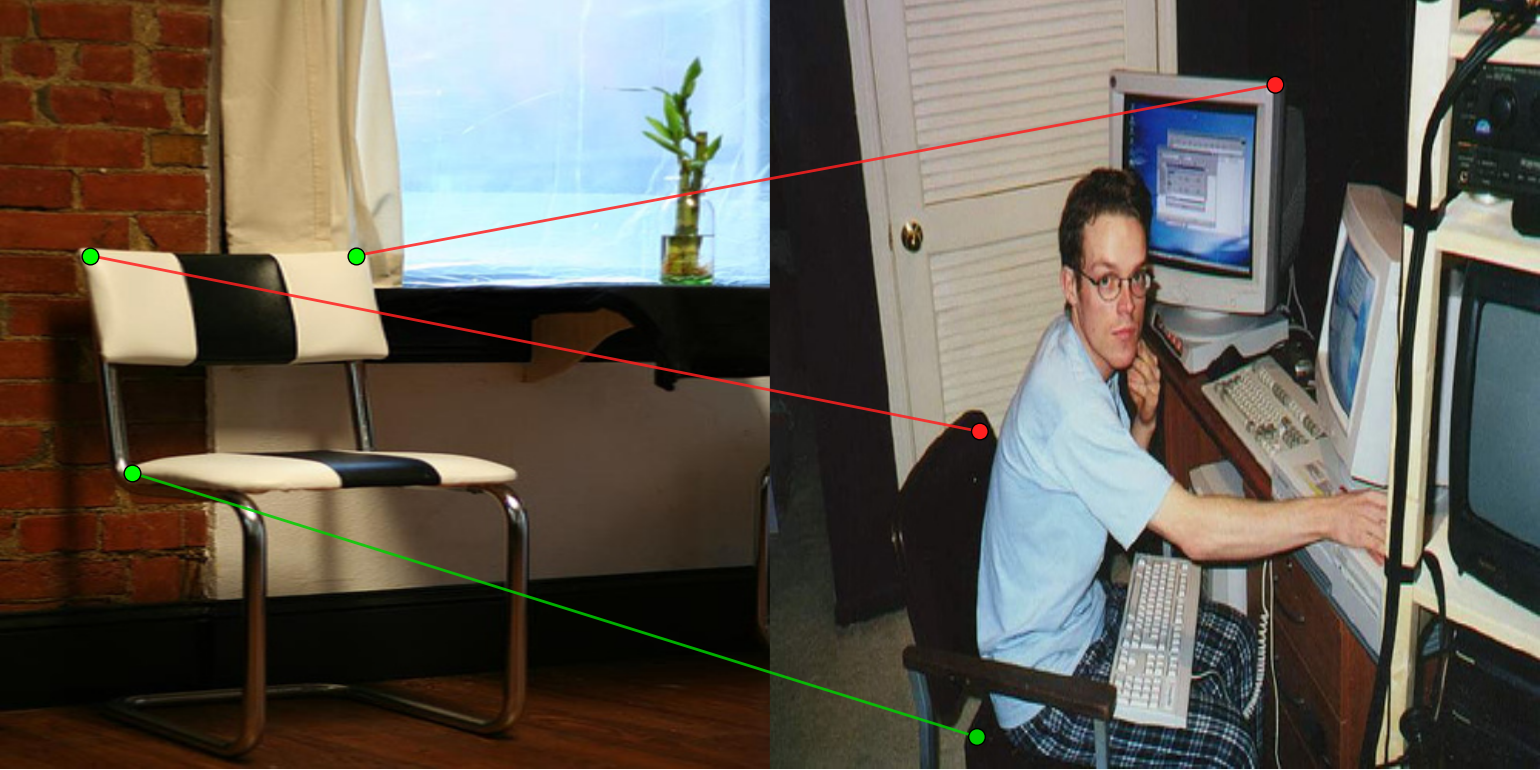
\includegraphics[width=0.48\textwidth]{figures/qualitative/marco/match_real_chair.png} &
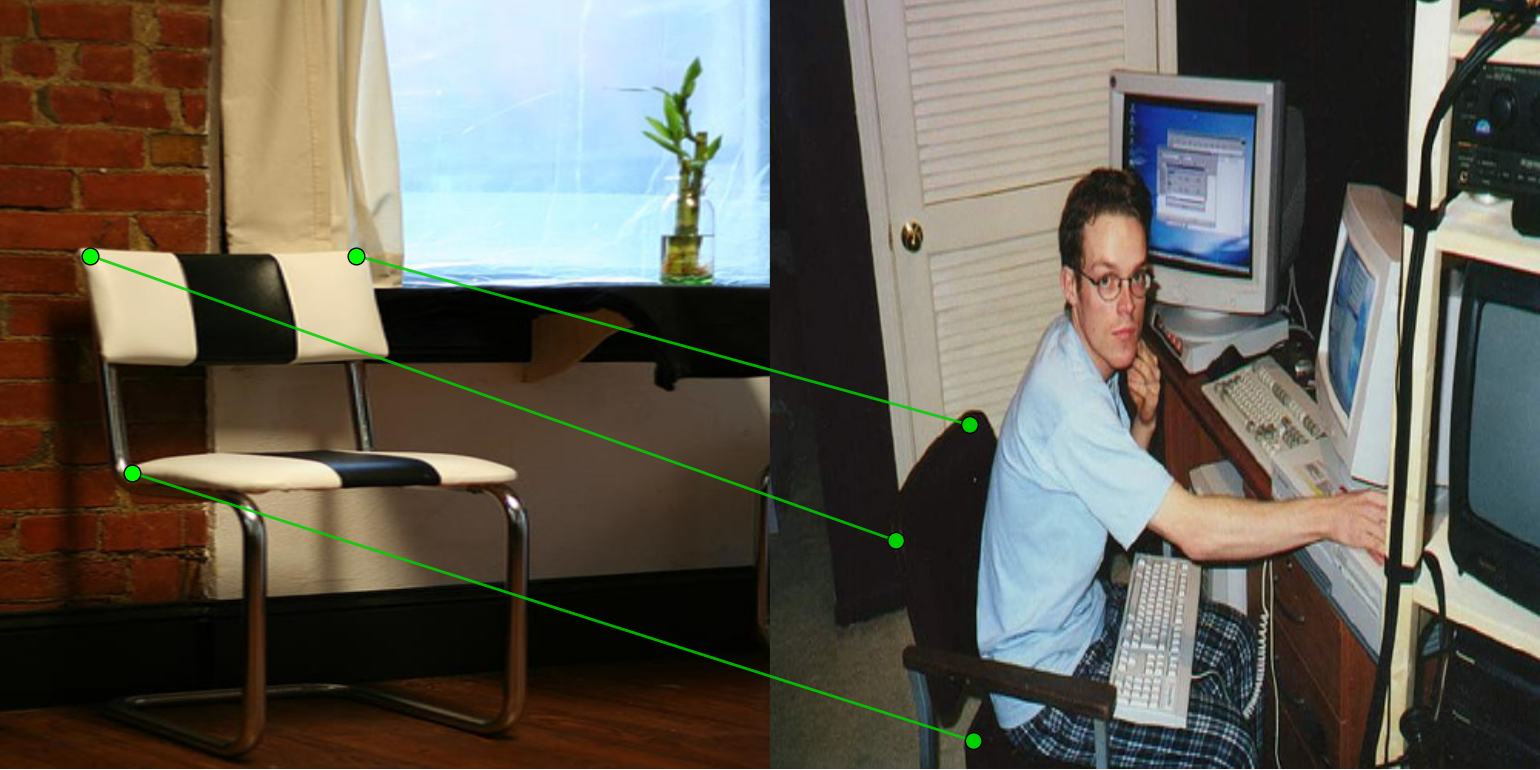
\includegraphics[width=0.48\textwidth]{figures/qualitative/marco/match_ours_chair.png} \\
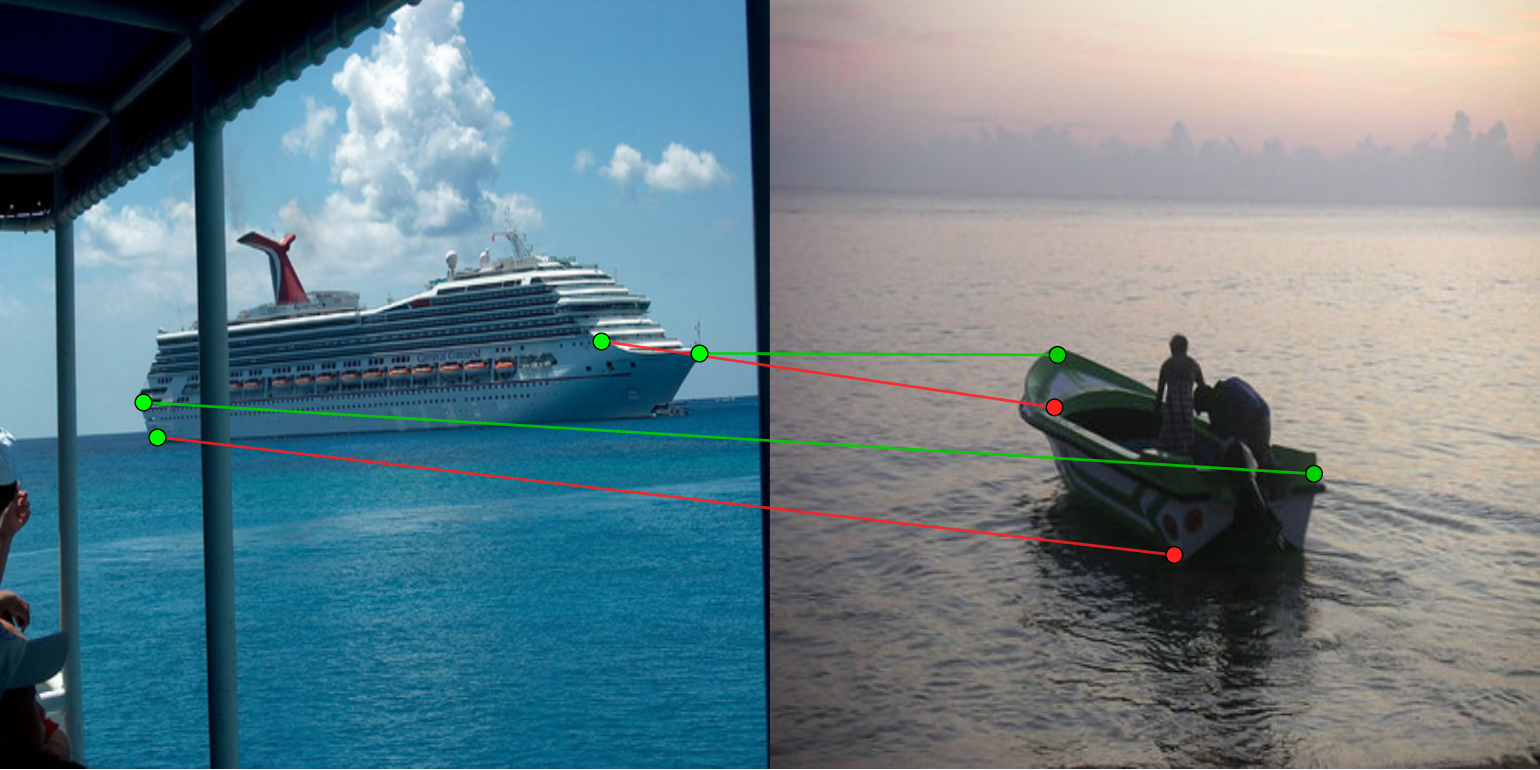
\includegraphics[width=0.48\textwidth]{figures/qualitative/marco/match_real_boat.png} &
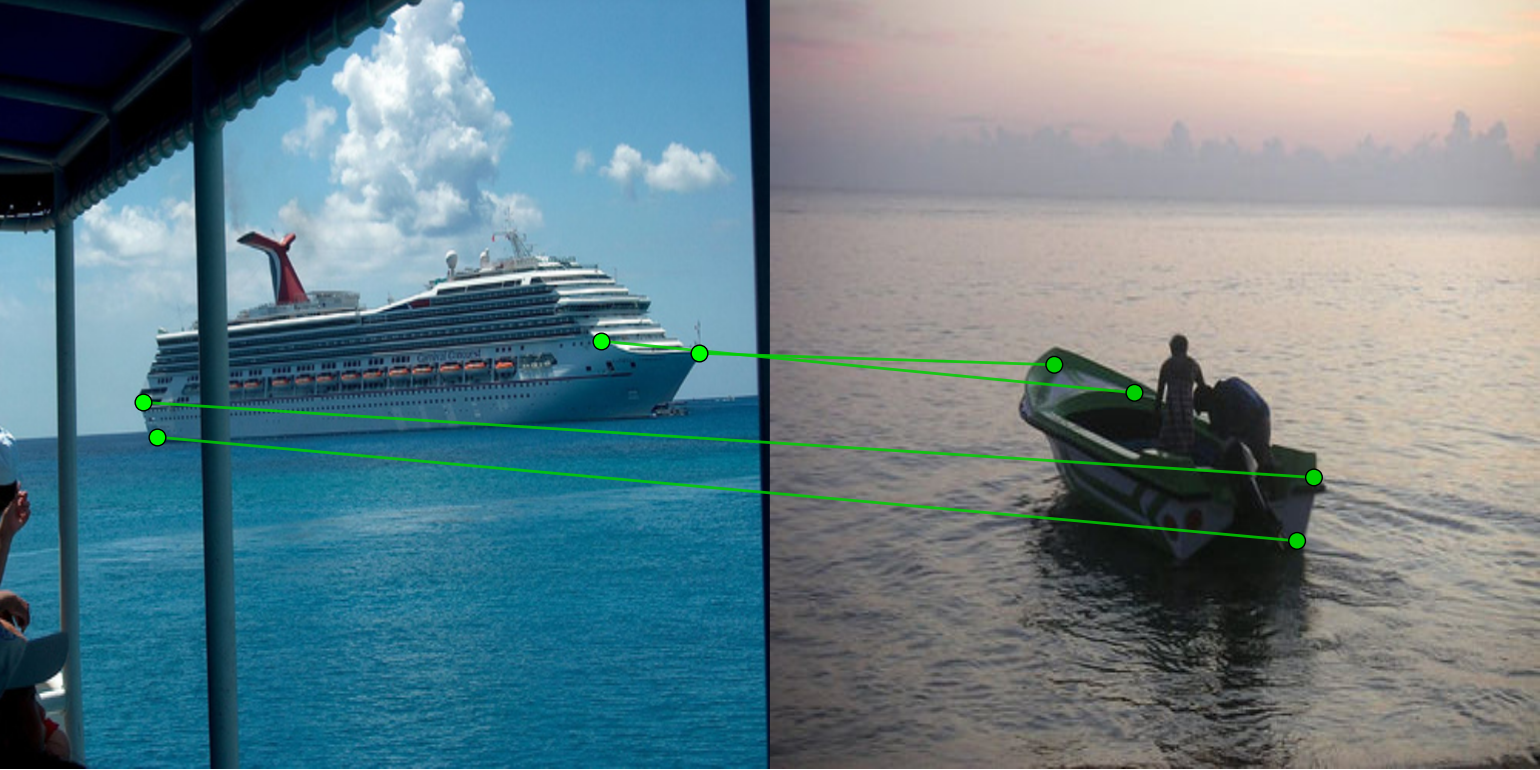
\includegraphics[width=0.48\textwidth]{figures/qualitative/marco/match_ours_boat.png} \\
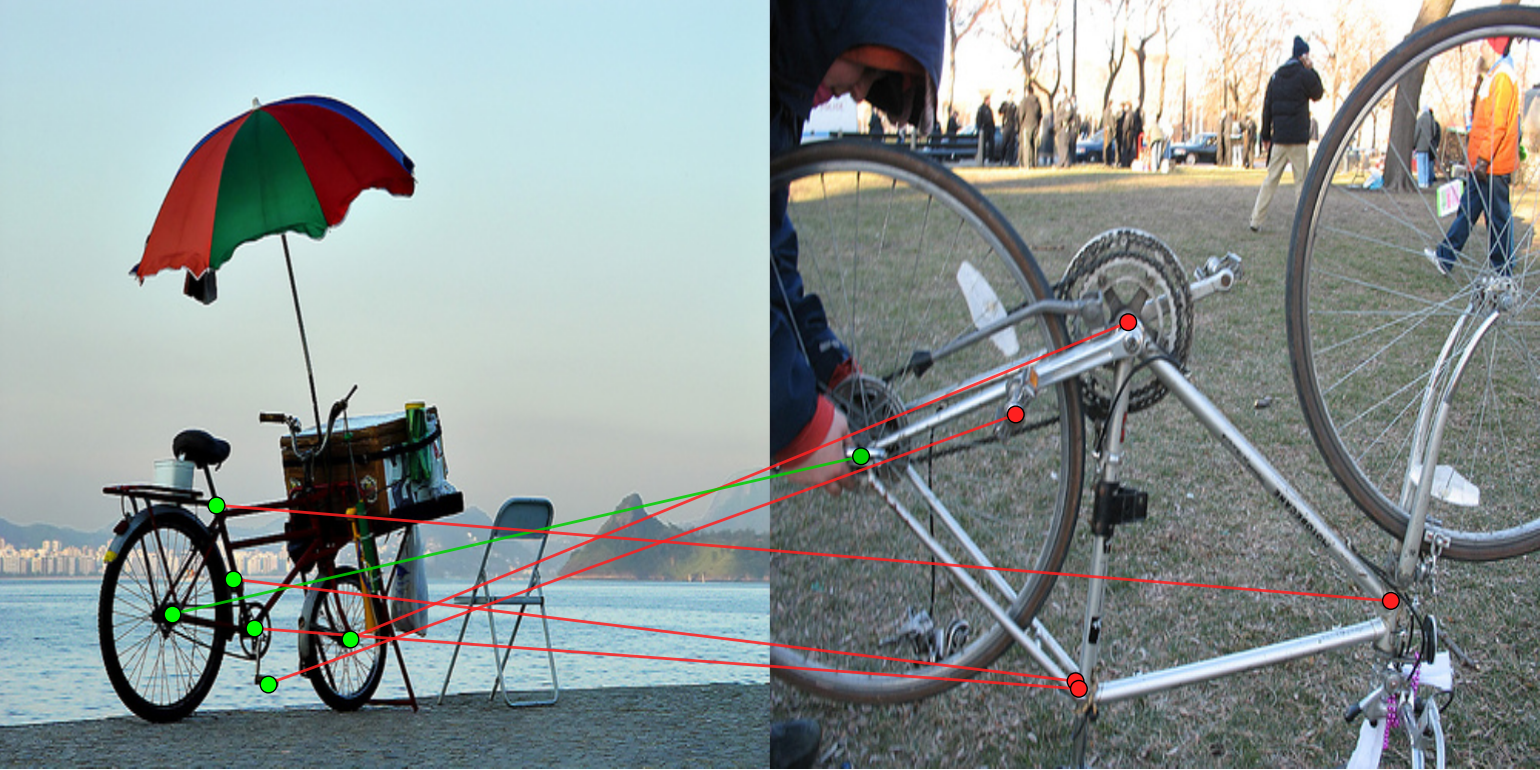
\includegraphics[width=0.48\textwidth]{figures/qualitative/marco/match_real_bicycle.png} &
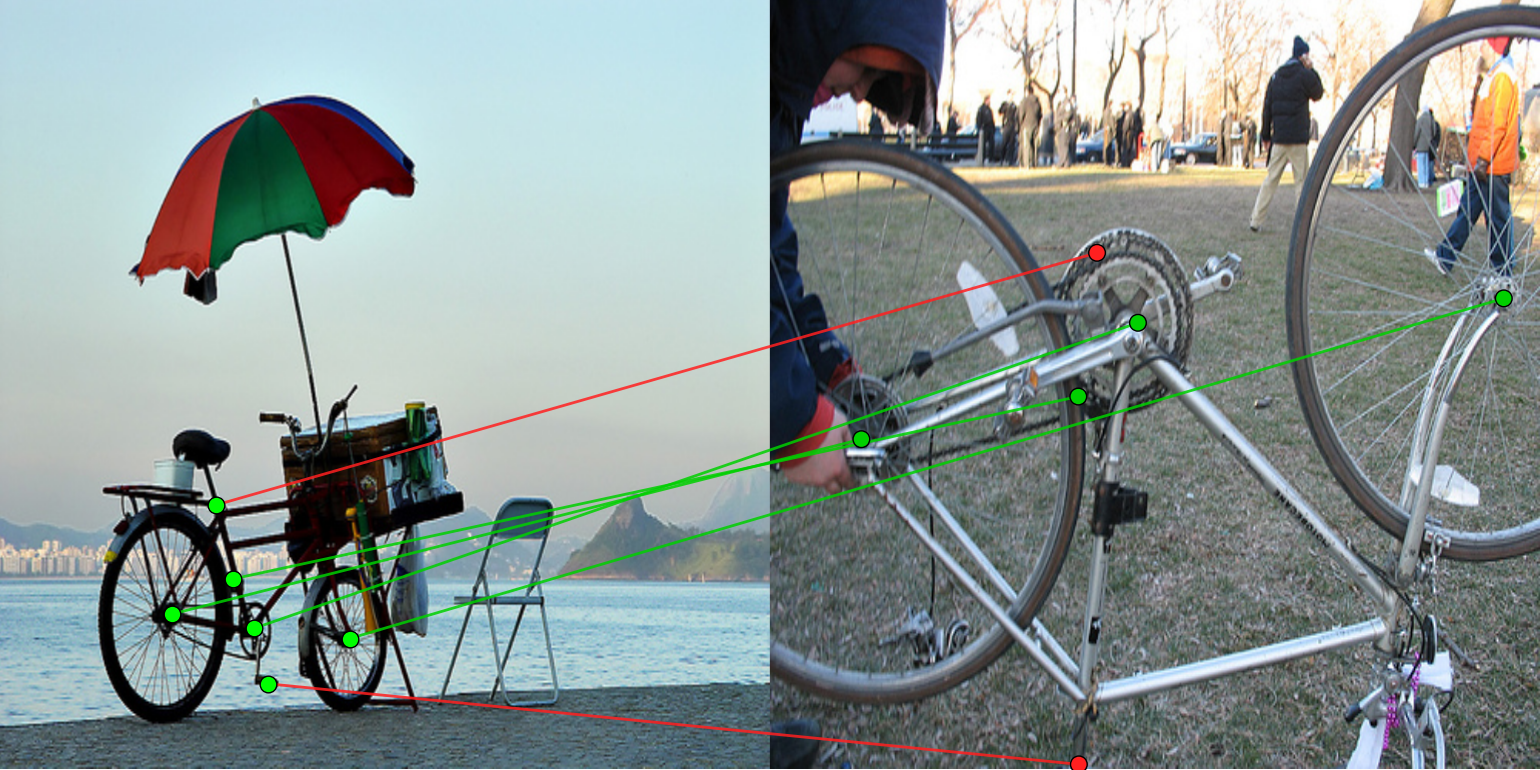
\includegraphics[width=0.48\textwidth]{figures/qualitative/marco/match_ours_bicycle.png} \\
\end{tabular}
\caption{\textbf{Qualitative SPair-71k \cite{min2019spair71k} results for MARCO \cite{cuttano2026marco}.}
Each image shows a source--target pair with predicted correspondences. We compare MARCO trained on SPair-71k against MARCO pretrained on our generated correspondences and then fine-tuned on SPair-71k.}
\label{fig:qual_marco}
\end{figure*}


\begin{figure*}[t]
\centering
\setlength{\tabcolsep}{3pt}
\begin{tabular}{cc}
\textbf{GeoAware-SC Real-only} & \textbf{GeoAware-SC Ours P.T.$\rightarrow$Real} \\
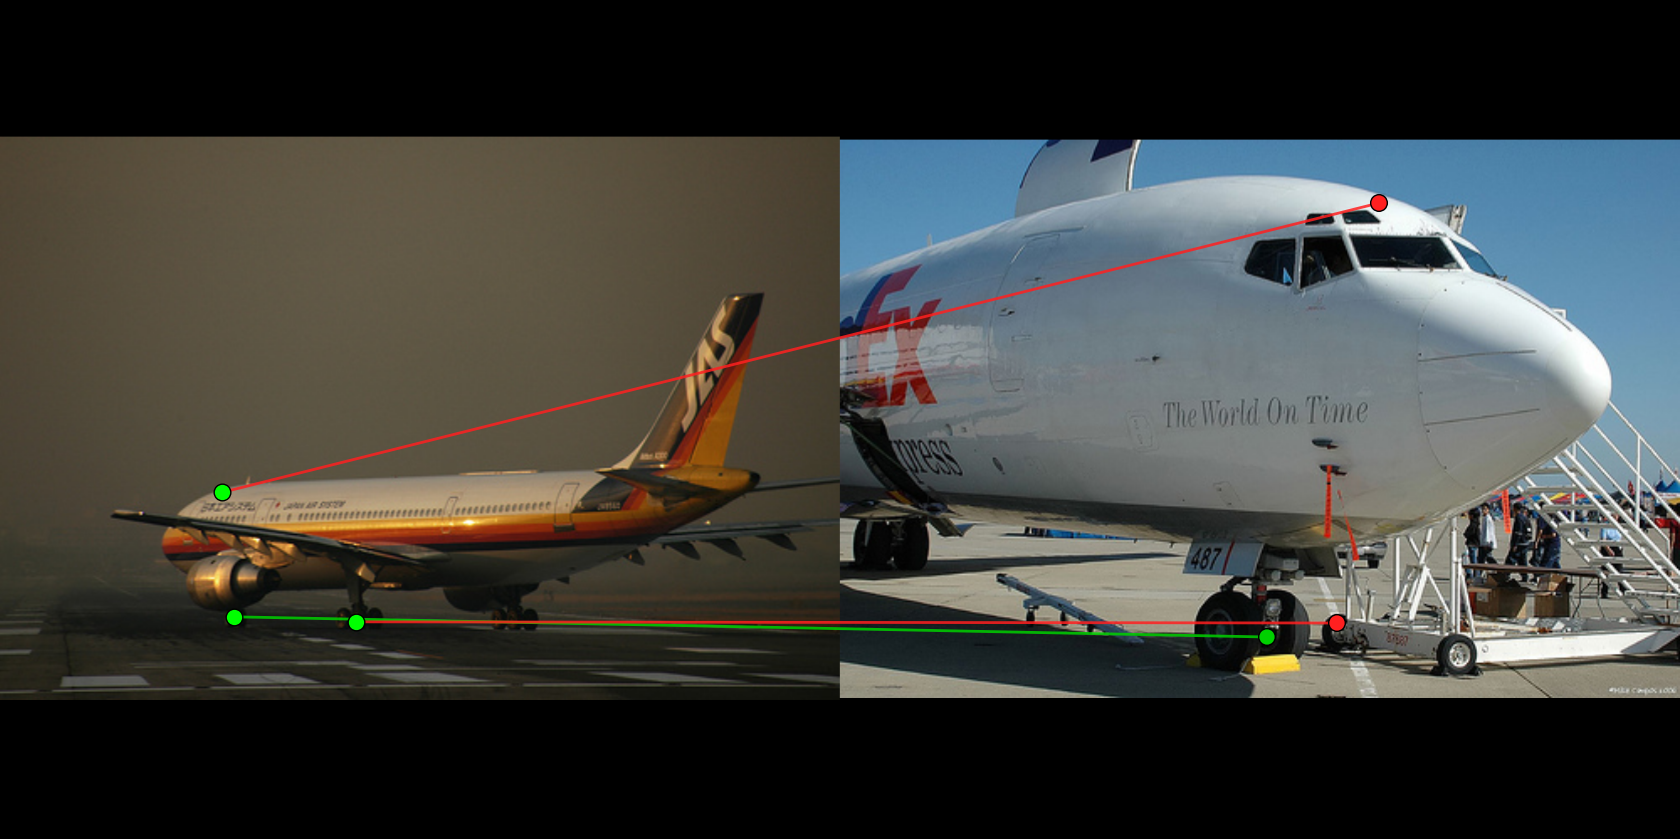
\includegraphics[width=0.48\textwidth]{figures/qualitative/geoaware/match_real_airplane.png} &
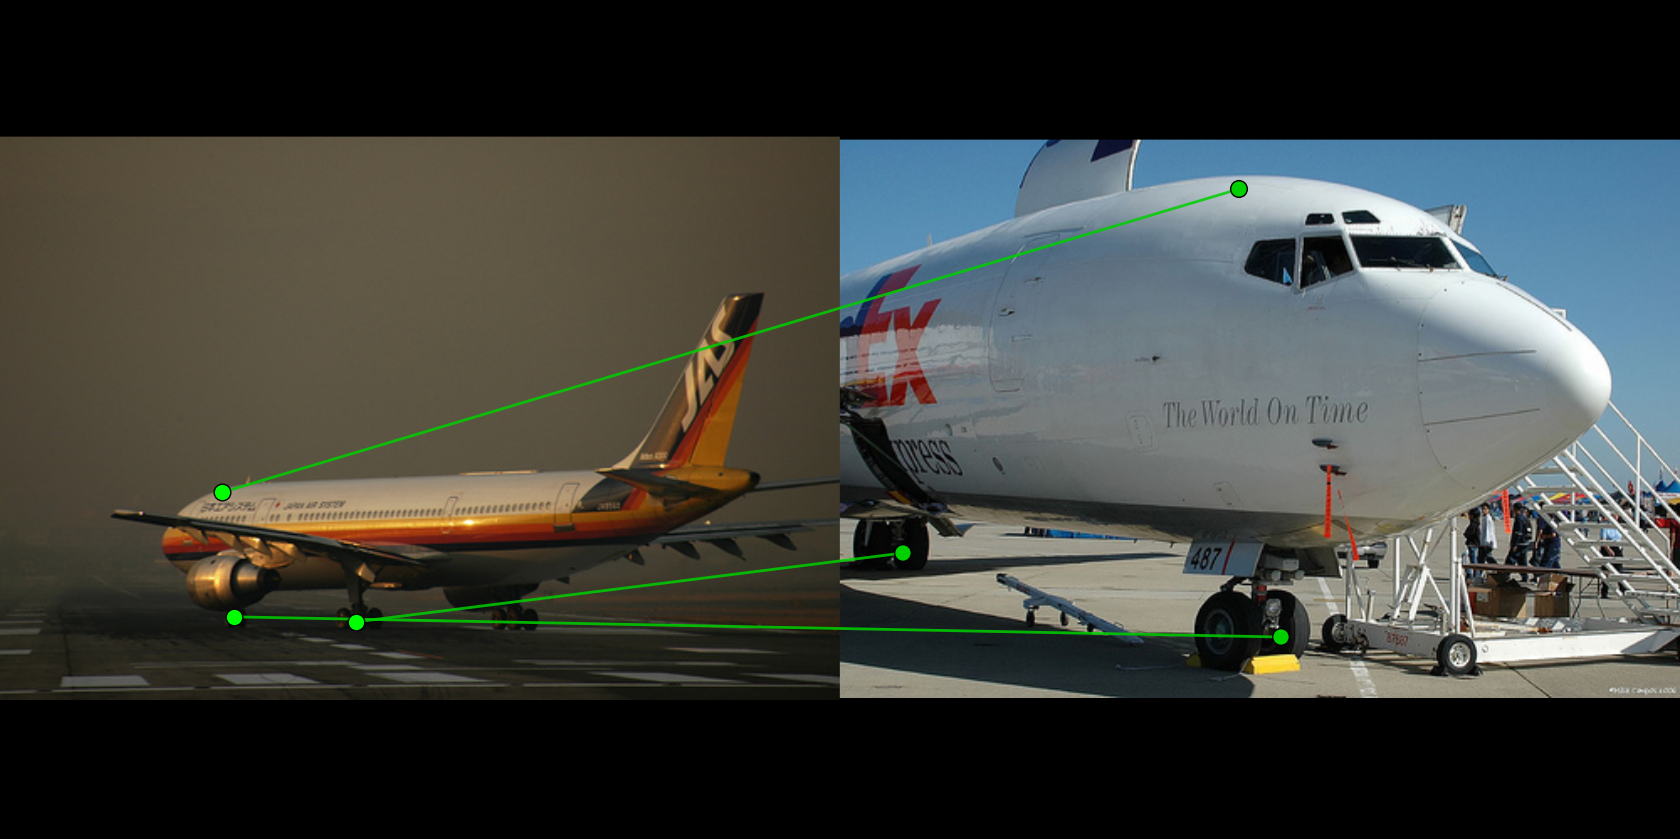
\includegraphics[width=0.48\textwidth]{figures/qualitative/geoaware/match_ours_airplane.png} \\
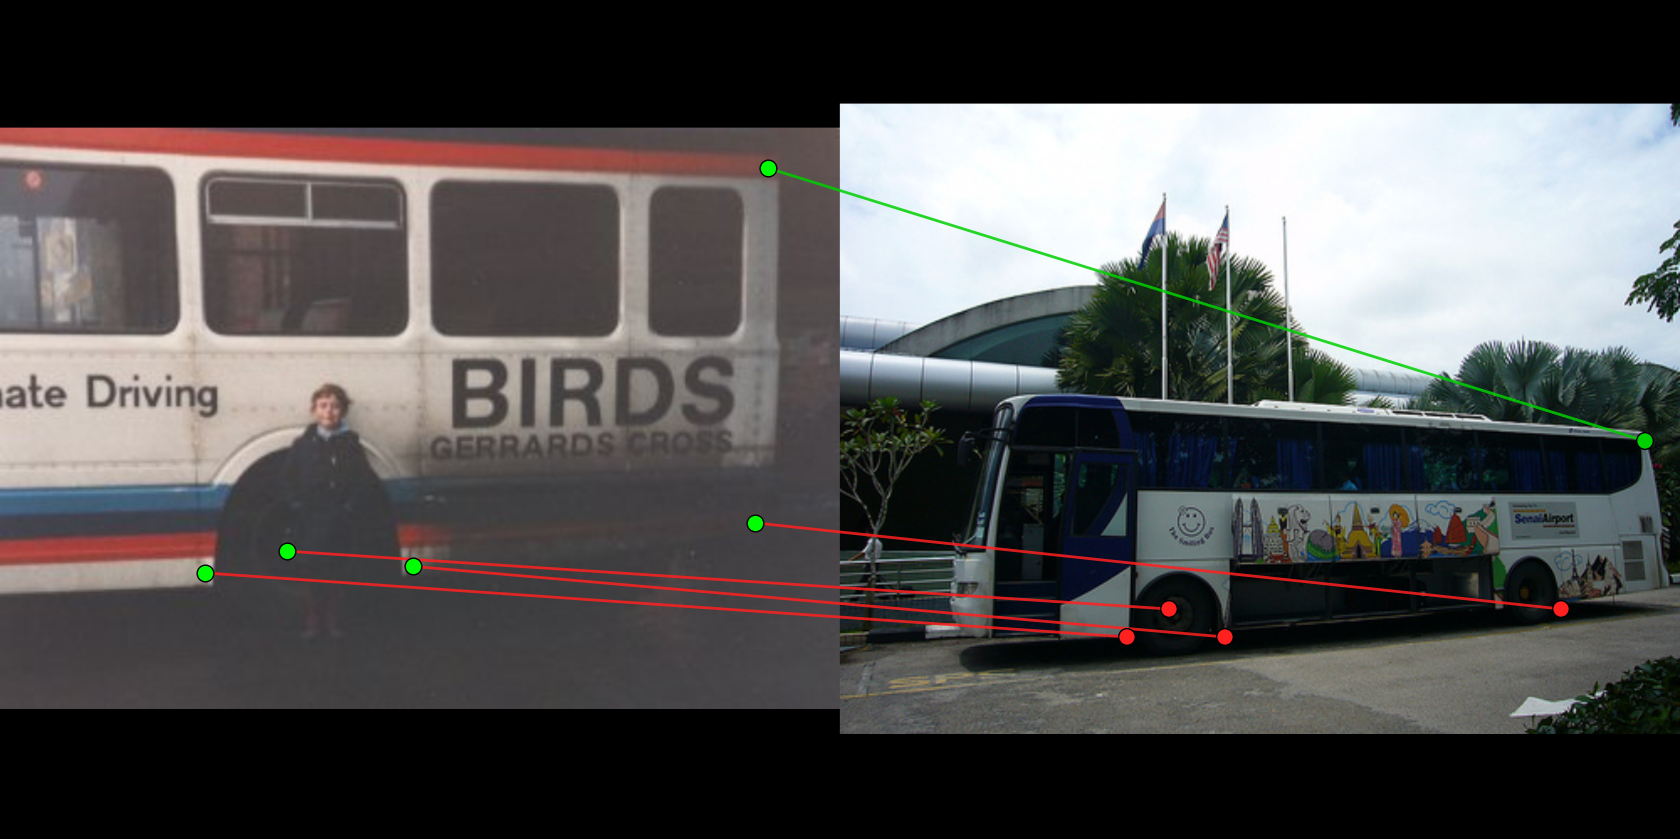
\includegraphics[width=0.48\textwidth]{figures/qualitative/geoaware/match_real_bus.png} &
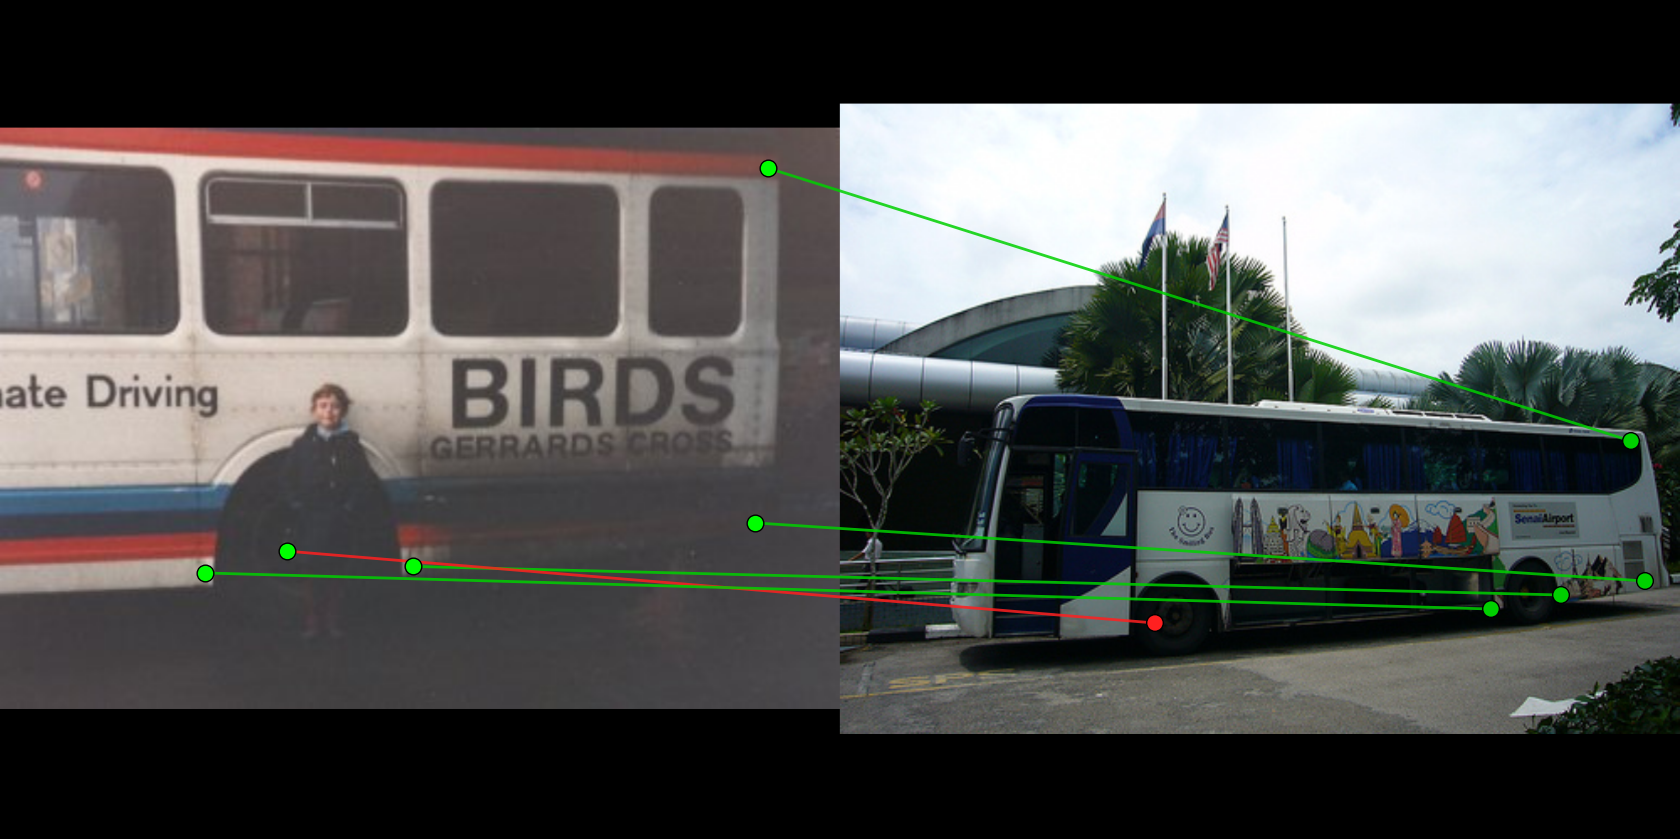
\includegraphics[width=0.48\textwidth]{figures/qualitative/geoaware/match_ours_bus.png} \\
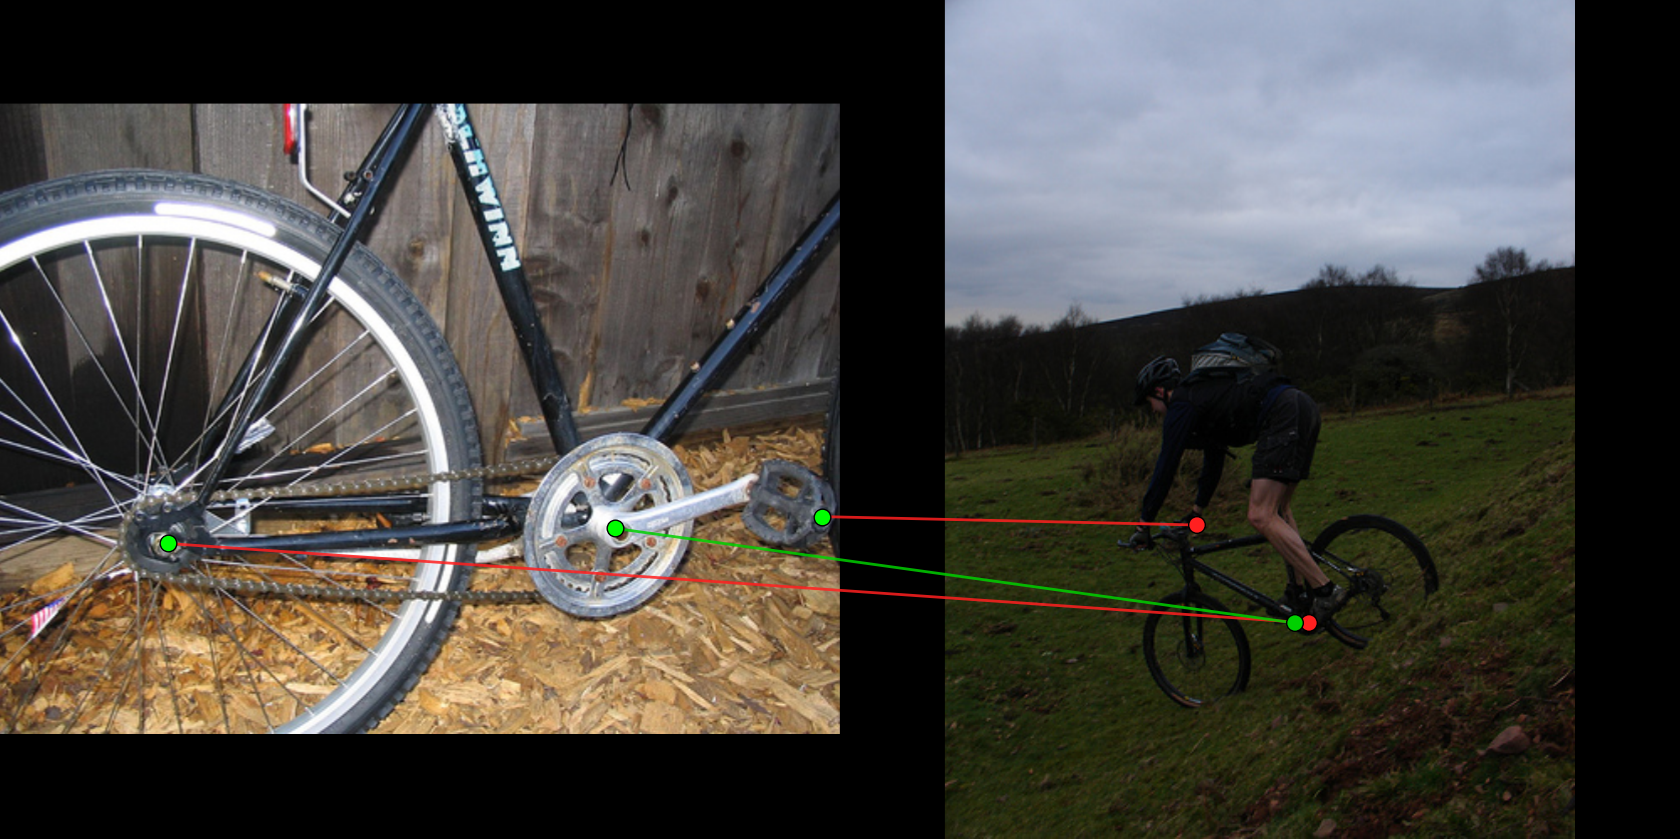
\includegraphics[width=0.48\textwidth]{figures/qualitative/geoaware/match_real_bike.png} &
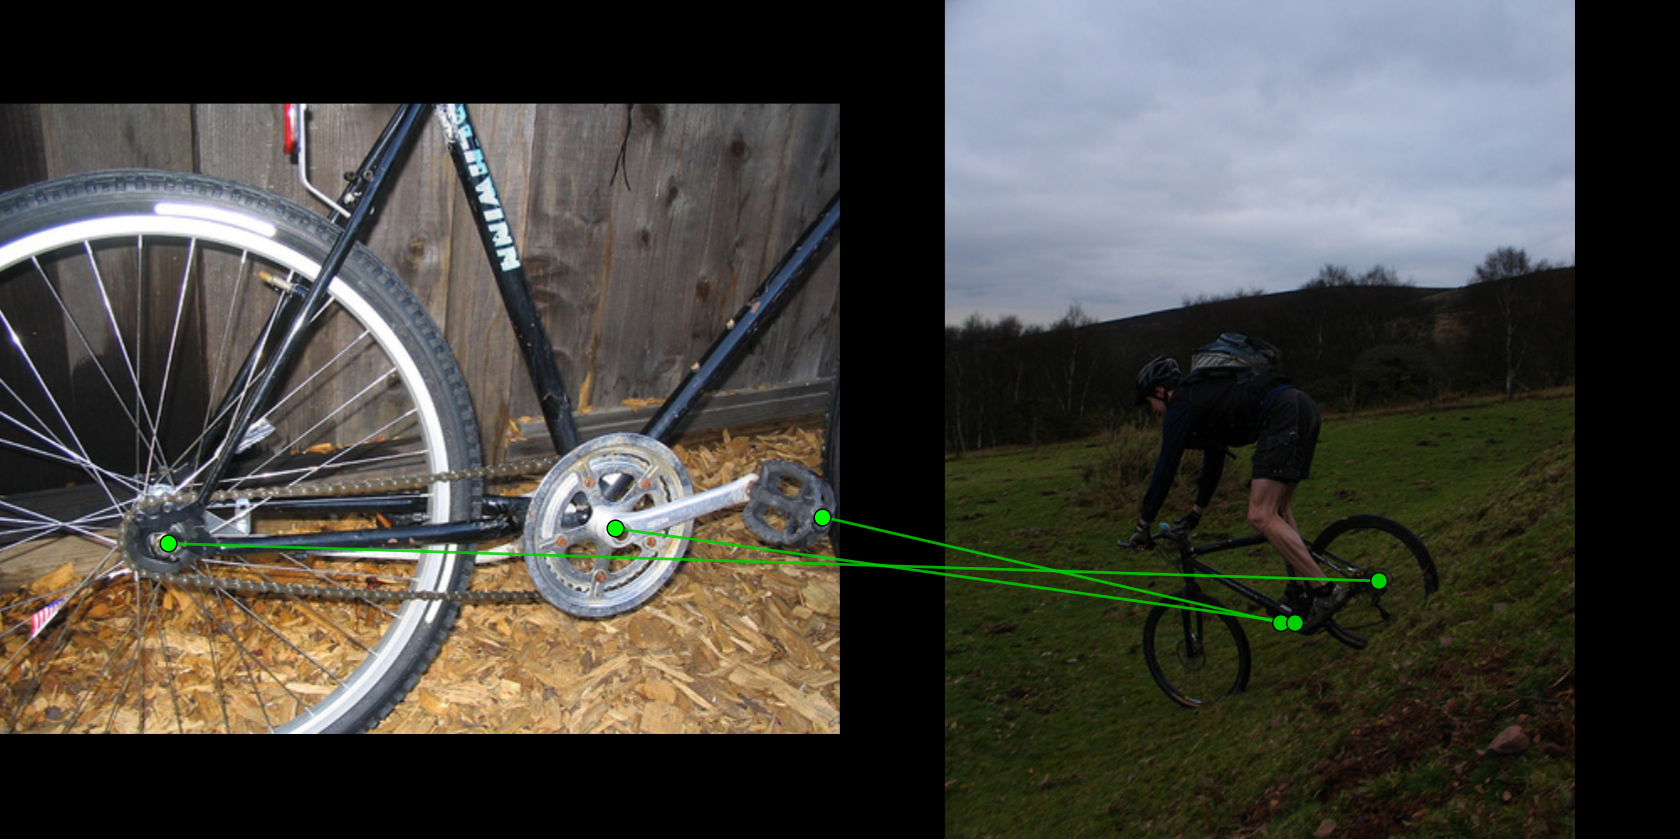
\includegraphics[width=0.48\textwidth]{figures/qualitative/geoaware/match_ours_bike.png} \\
\end{tabular}
\caption{\textbf{Qualitative SPair-71k \cite{min2019spair71k} results for GeoAware-SC \cite{zhang2024tellingLeftFromRight}.}
Each image shows a source--target pair with predicted correspondences. We compare GeoAware-SC trained on SPair-71k against GeoAware-SC pretrained on our generated correspondences and then fine-tuned on SPair-71k.}
\label{fig:qual_geoaware}
\end{figure*}

\clearpage
\subsection{Correspondence Examples on New Categories}

We additionally show (\autoref{fig:new_categories_examples}) qualitative correspondence examples on rigid categories beyond those covered by existing correspondence benchmarks such as SPair-71k \cite{min2019spair71k}, KeypointNet \cite{you2020}, and AP-10K \cite{yu2021AP10k}. These examples demonstrate the ability of our method to establish approximate semantic-geometric correspondences on diverse categories from Objaverse-OA \cite{orient_anything}.

\begin{figure*}[h]
\centering
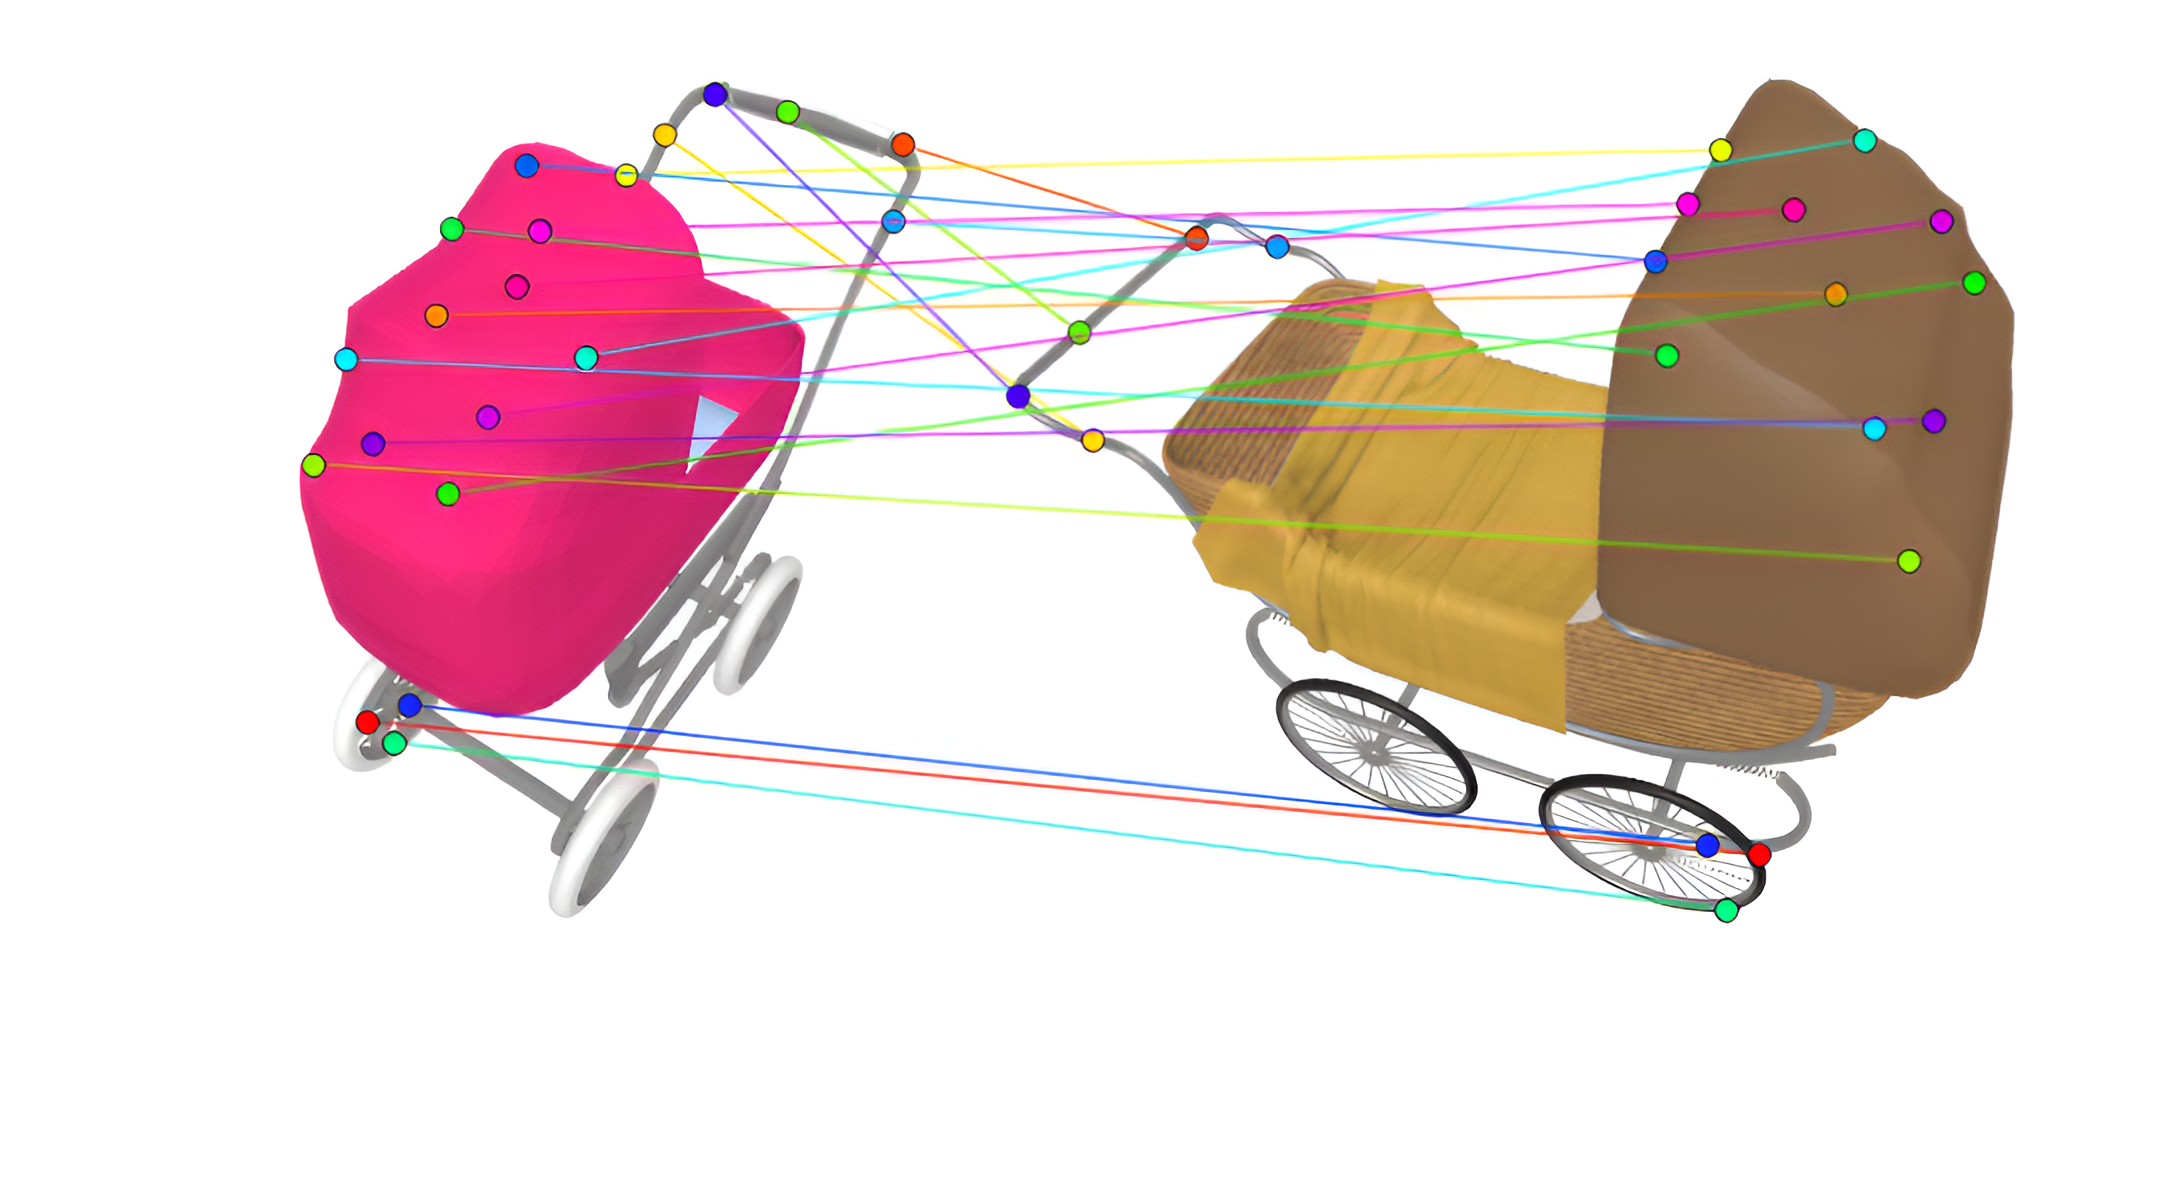
\includegraphics[width=0.92\linewidth,height=0.22\textheight,keepaspectratio,trim={100 150 100 40},clip]{figures/matching_examples/baby_buggy_highres.png}\vspace{1mm}

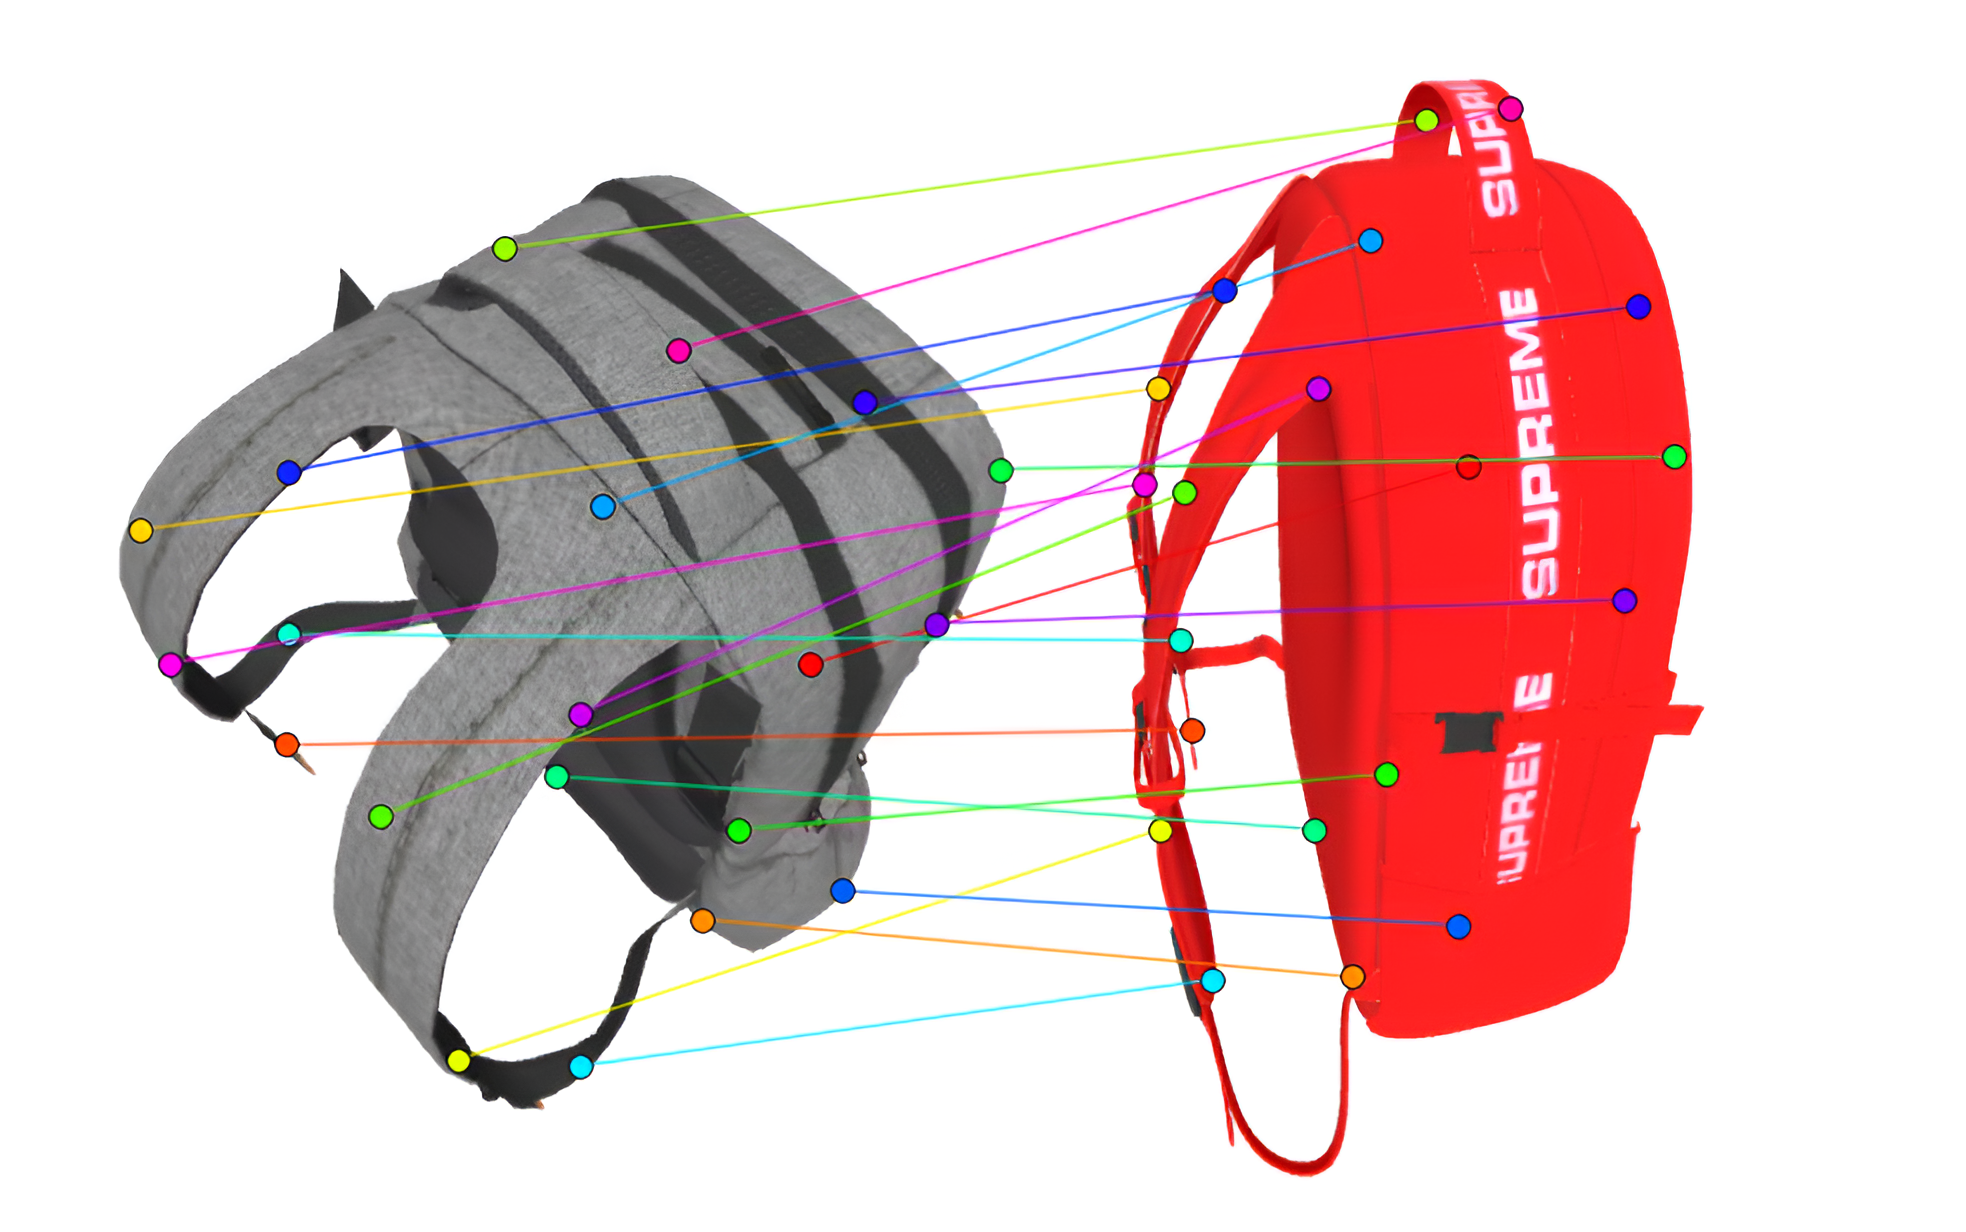
\includegraphics[width=0.92\linewidth,height=0.22\textheight,keepaspectratio,trim={0 20 70 40},clip]{figures/matching_examples/backpack_highres.png}\vspace{1mm}

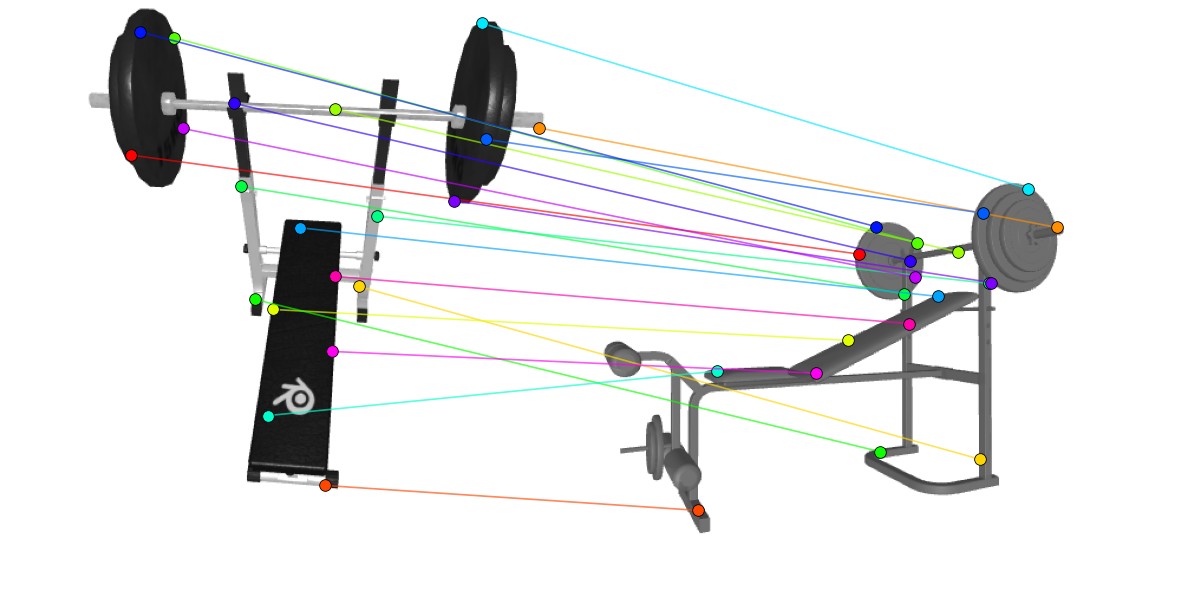
\includegraphics[width=0.92\linewidth,height=0.22\textheight,keepaspectratio,trim={0 45 50 0},clip]{figures/matching_examples/barbell.png}

\caption{
Qualitative correspondence examples on categories beyond existing correspondence benchmarks. Colors indicate sampled semantic-geometric correspondences established by our method.
}
\label{fig:new_categories_examples}
\end{figure*}

% \begin{figure*}[t]
% \centering
% 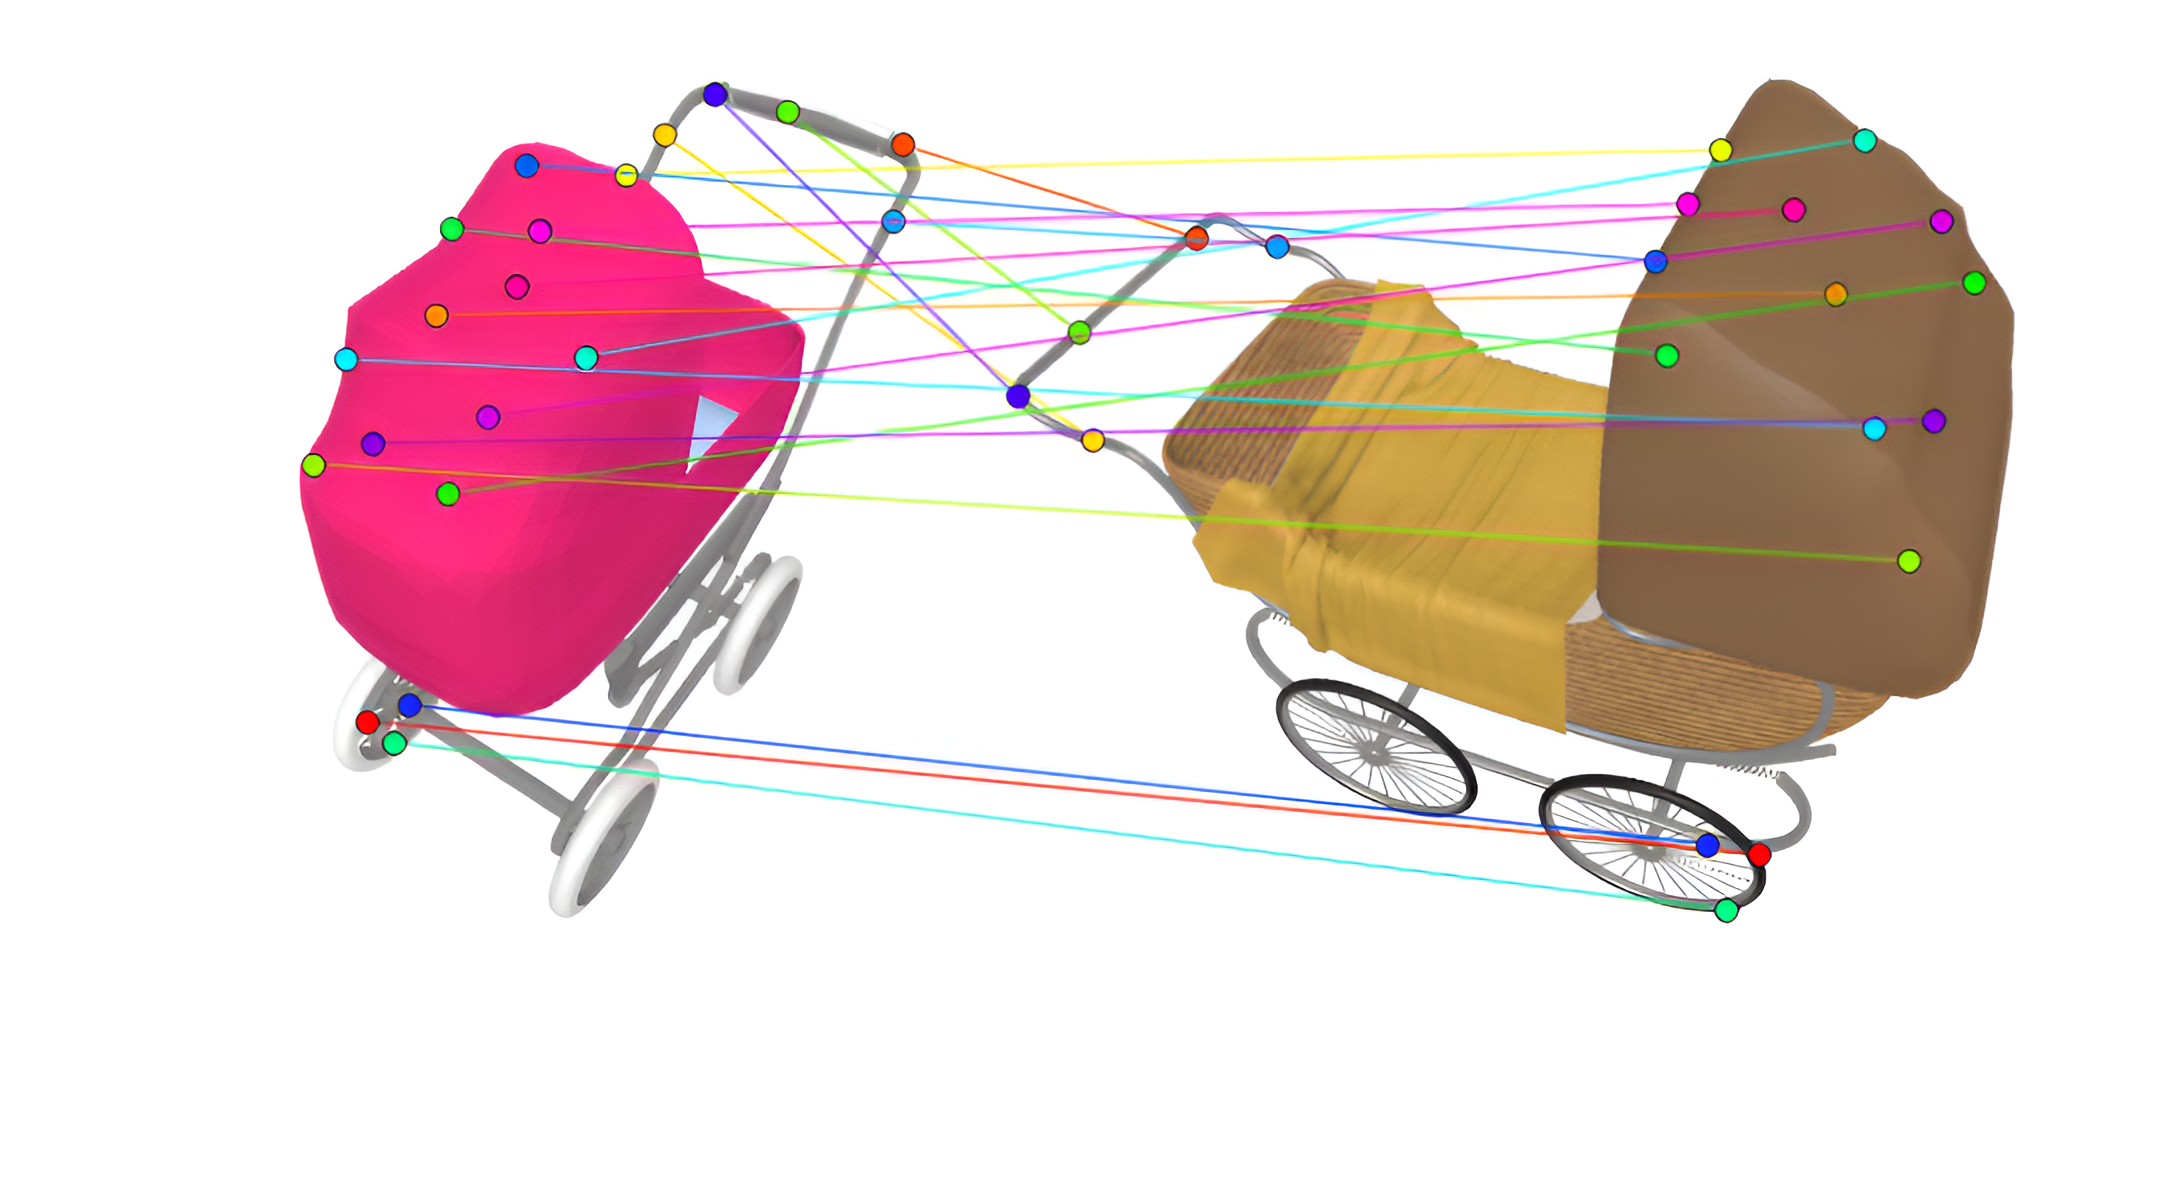
\includegraphics[width=\linewidth,height=\kpimgheight,trim={100 150 100 40},clip]{figures/matching_examples/baby_buggy_highres.png}\vfill
% % 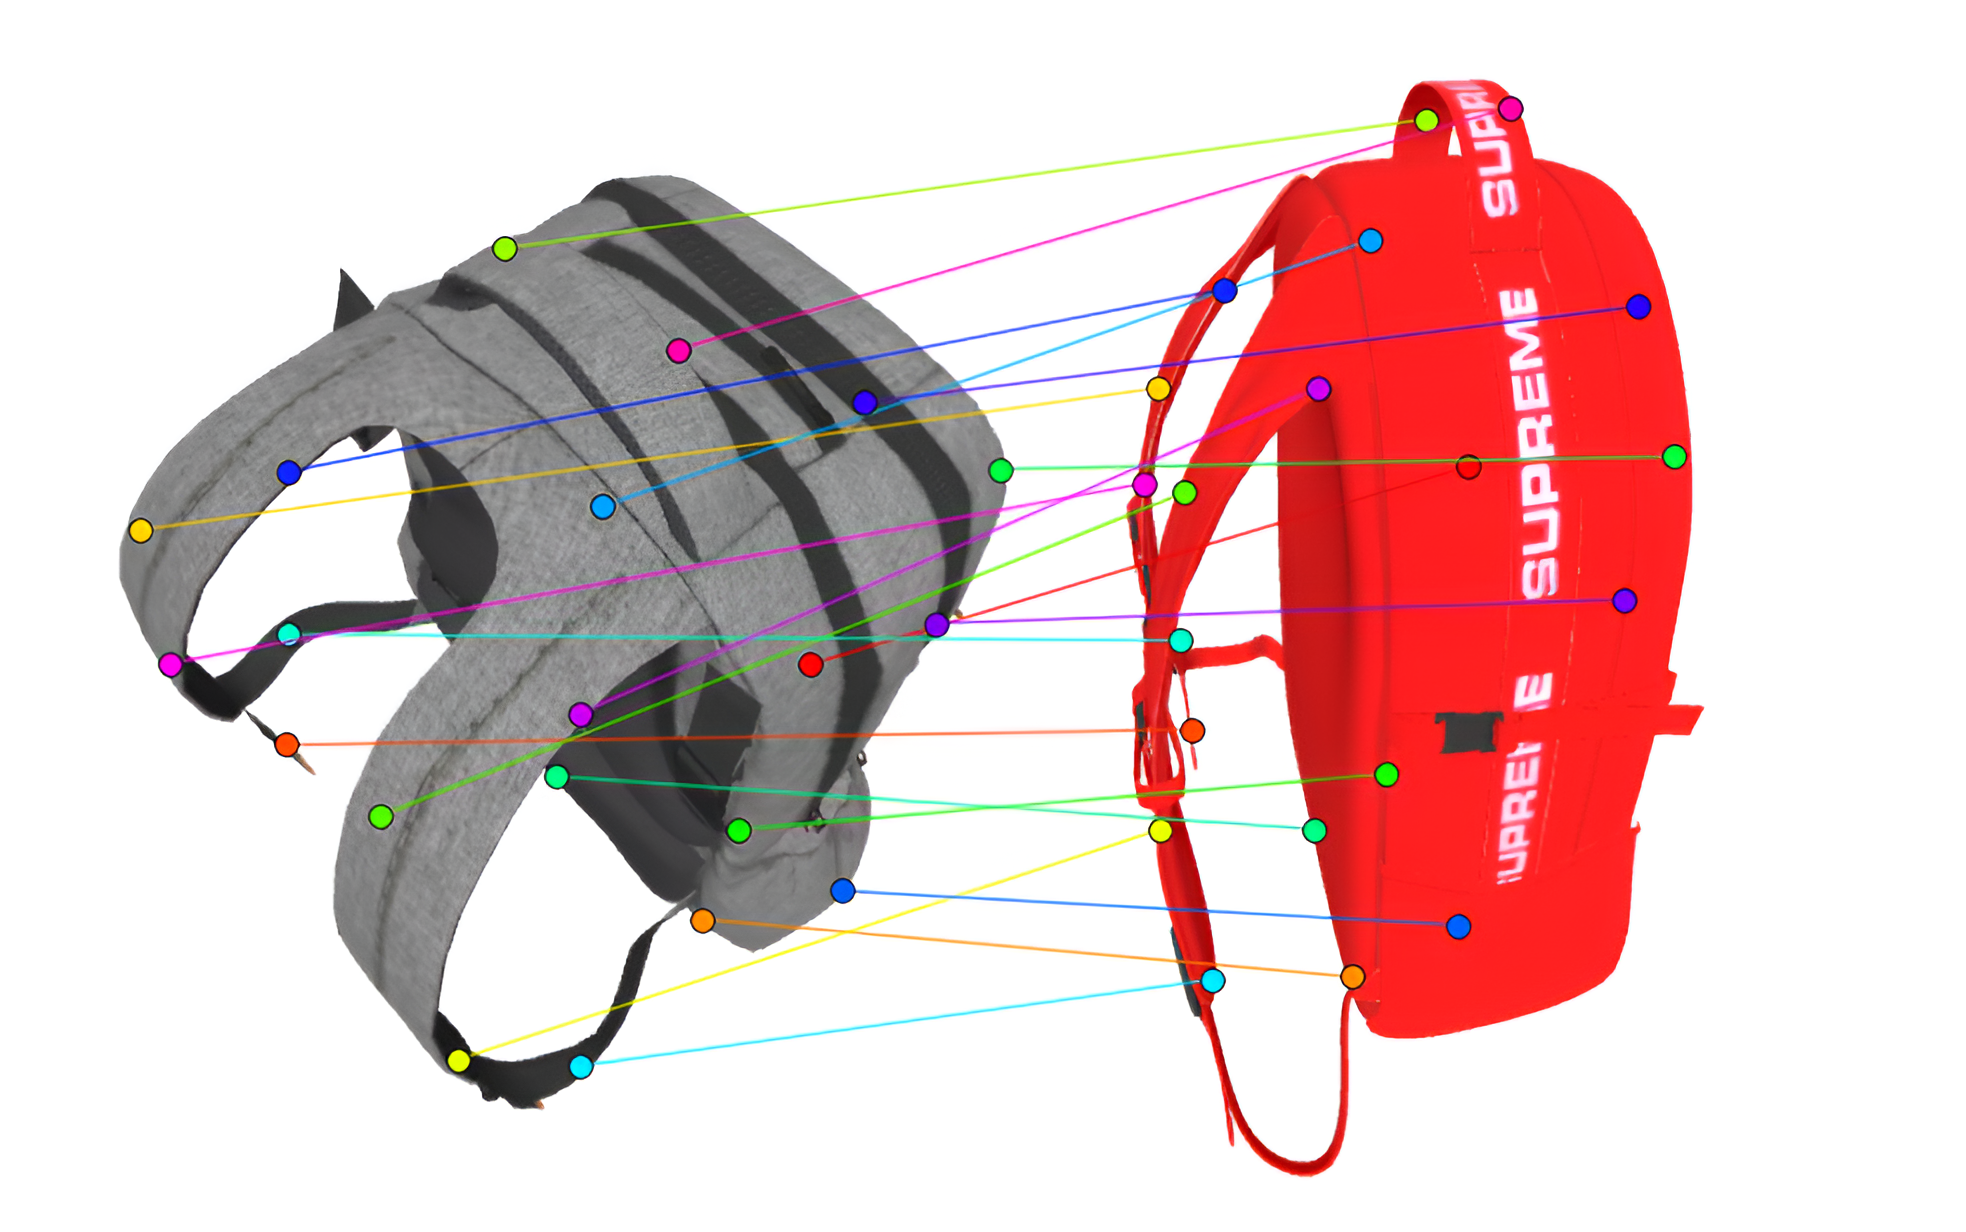
\includegraphics[width=\linewidth,height=\kpimgheight,trim={0 20 70 40},clip]{figures/matching_examples/backpack_highres.png}\vfill
% % 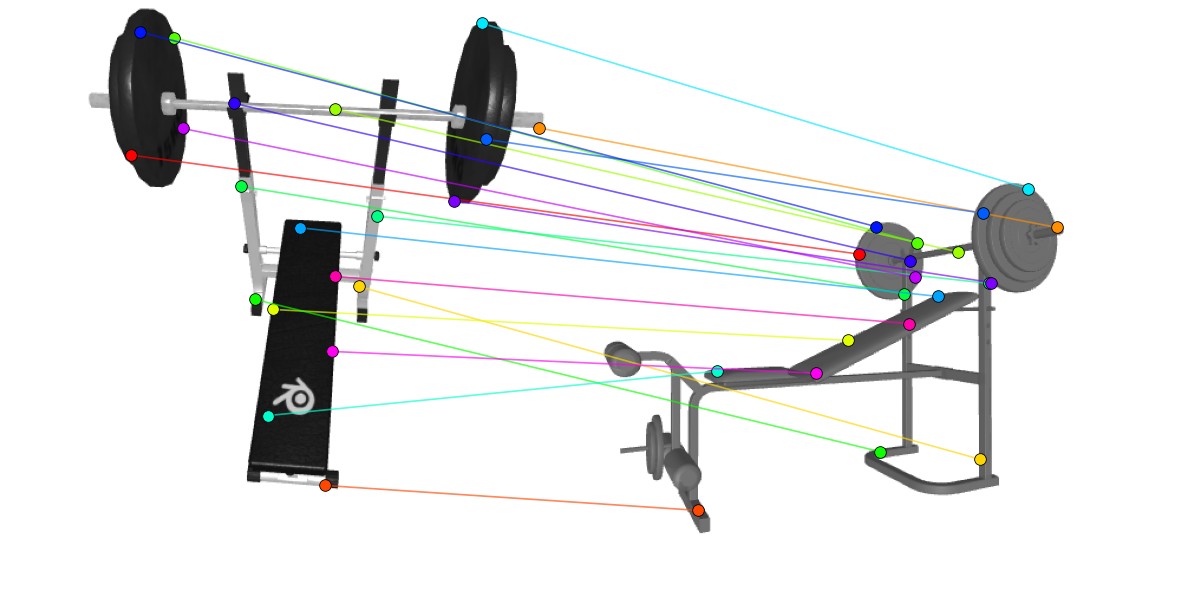
\includegraphics[width=\linewidth,height=\kpimgheight,trim={00 45 50 0},clip]{figures/matching_examples/barbell.png}
% \caption{
% Qualitative correspondence examples on categories beyond existing correspondence benchmarks. Colors indicate sampled semantic-geometric correspondences established by our method.

% We provide qualitative SPair-71k \cite{min2019spair71k} examples comparing models trained only on real SPair-71k annotations with the same models pretrained on our generated synthetic correspondences and then fine-tuned on SPair-71k. We show results for both MARCO \cite{cuttano2026marco} (see \autoref{fig:qual_marco}) and GeoAware-SC \cite{zhang2024tellingLeftFromRight} (see \autoref{fig:qual_geoaware}).


% \begin{figure*}[t]
% \centering
% \setlength{\tabcolsep}{3pt}
% \begin{tabular}{cc}
% \textbf{MARCO \cite{cuttano2026marco} Real-only} & \textbf{MARCO \cite{cuttano2026marco} Ours P.T.$\rightarrow$Real} \\
% 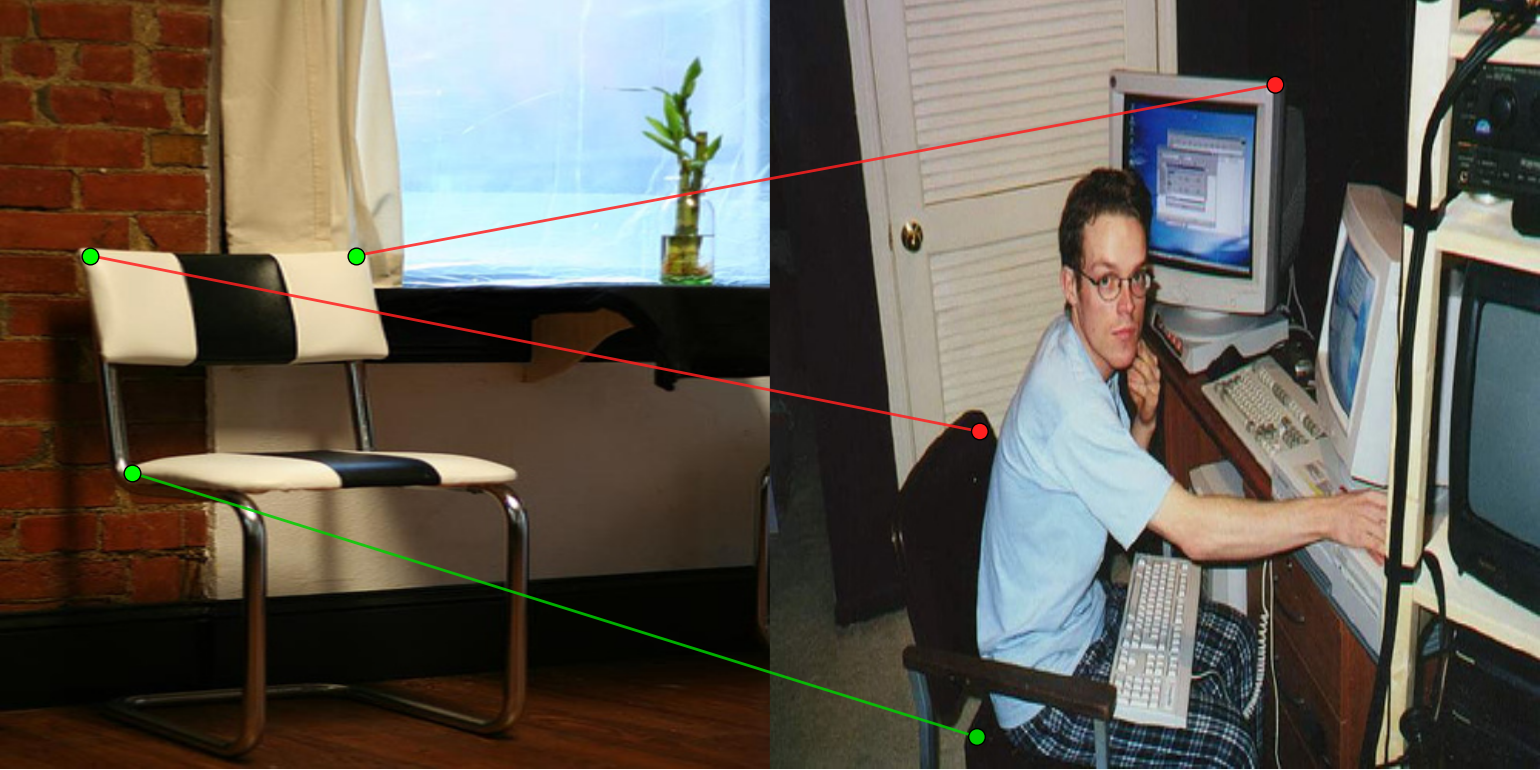
\includegraphics[width=0.48\textwidth]{figures/qualitative/marco/match_real_chair.png} &
% 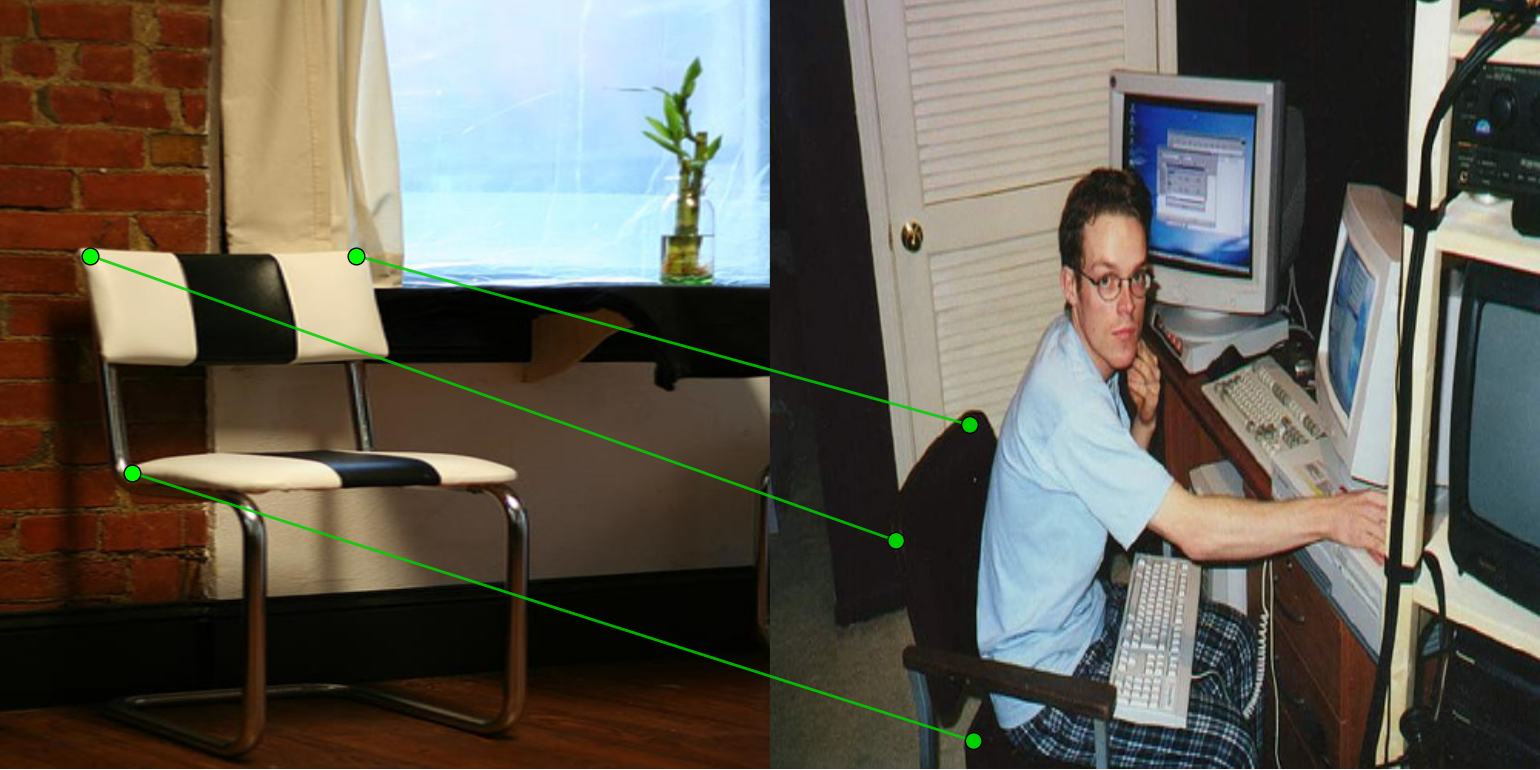
\includegraphics[width=0.48\textwidth]{figures/qualitative/marco/match_ours_chair.png} \\
% 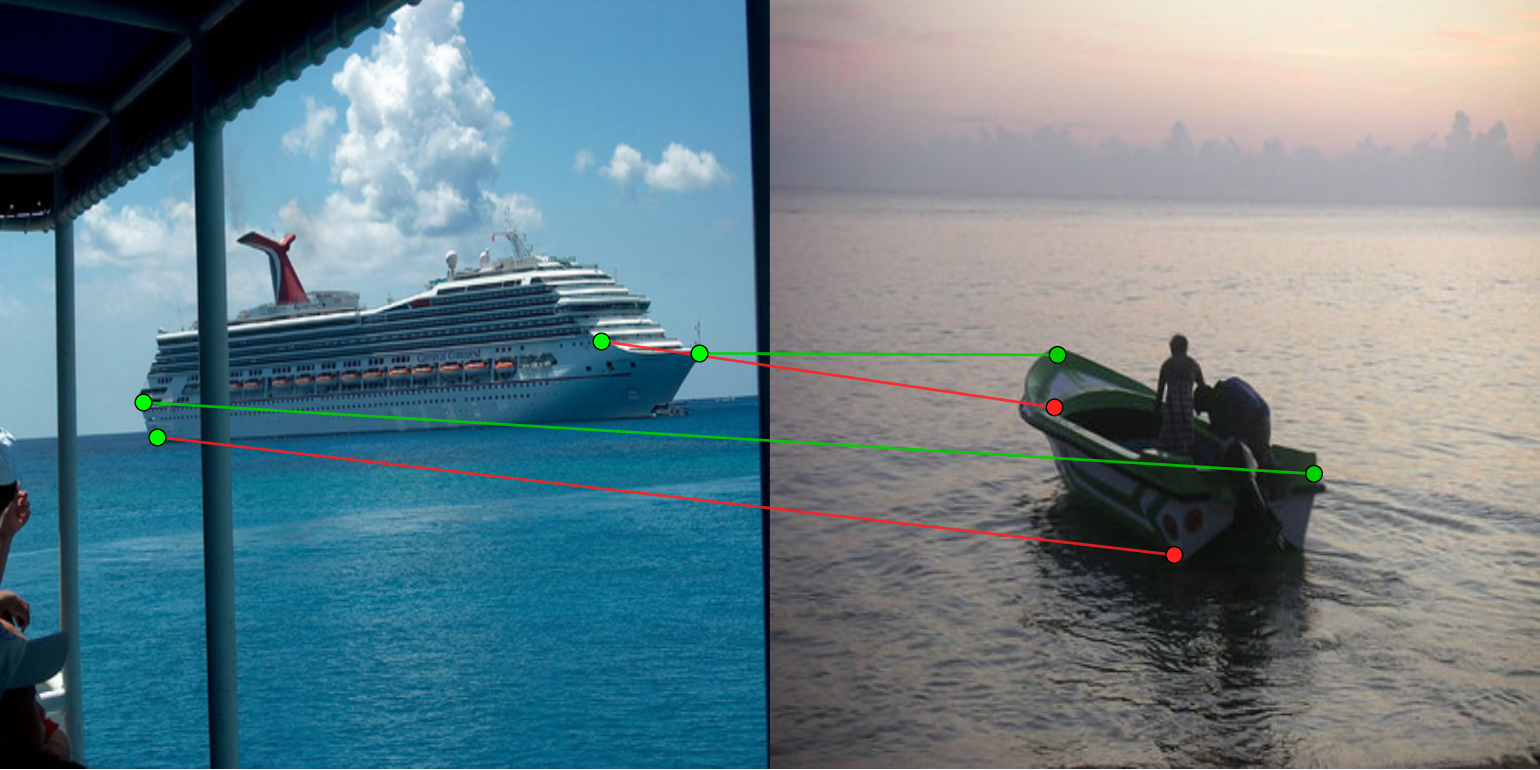
\includegraphics[width=0.48\textwidth]{figures/qualitative/marco/match_real_boat.png} &
% 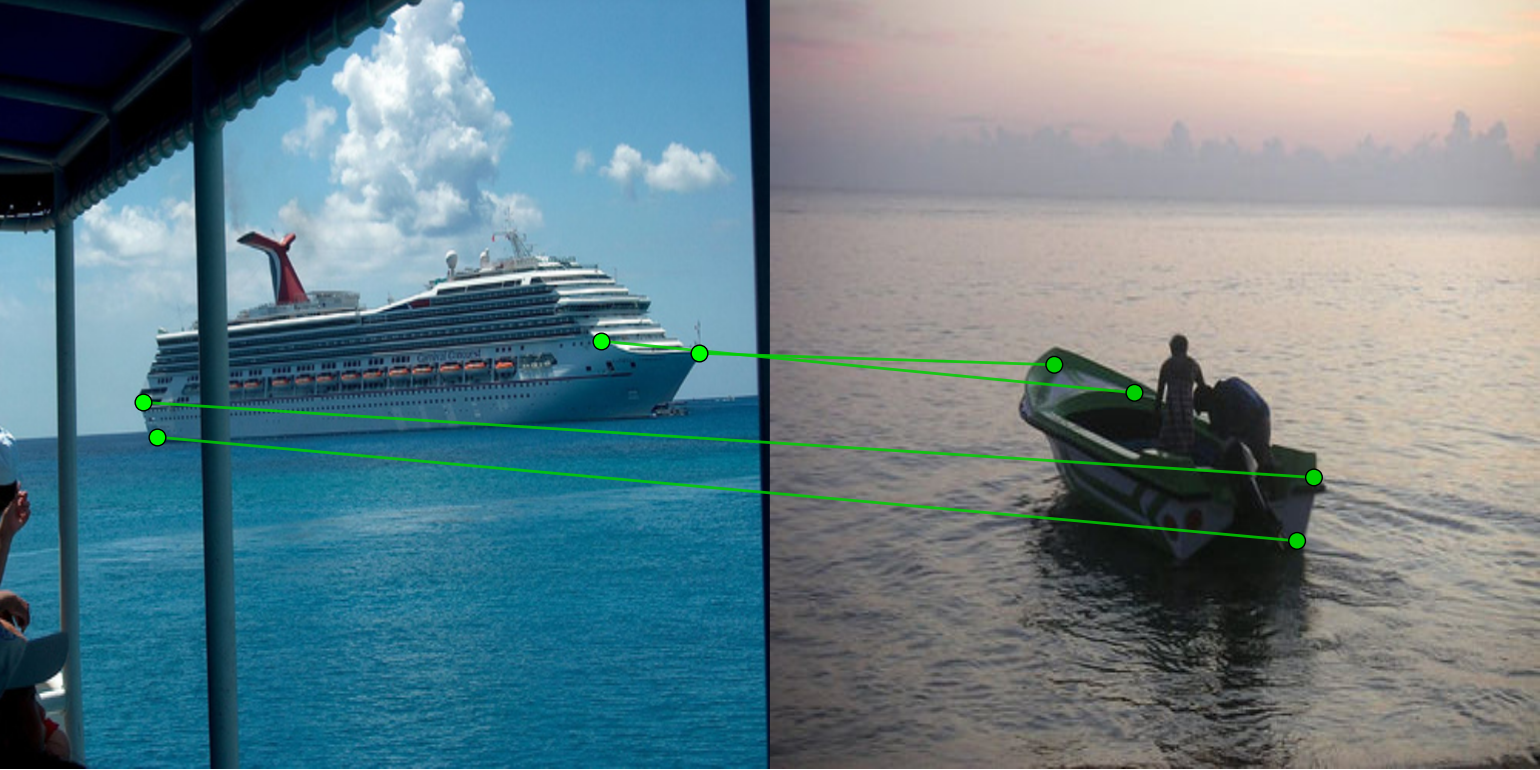
\includegraphics[width=0.48\textwidth]{figures/qualitative/marco/match_ours_boat.png} \\
% 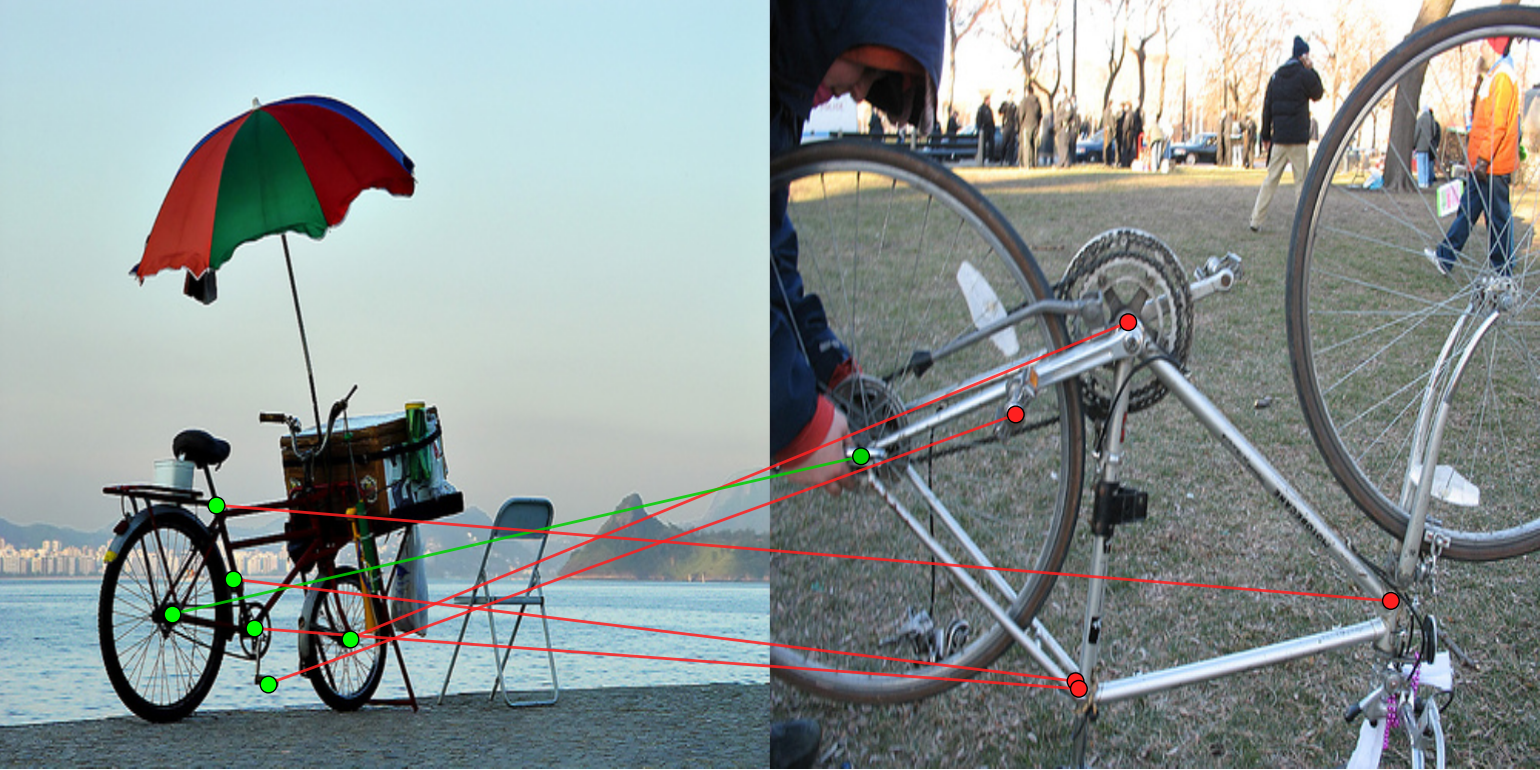
\includegraphics[width=0.48\textwidth]{figures/qualitative/marco/match_real_bicycle.png} &
% 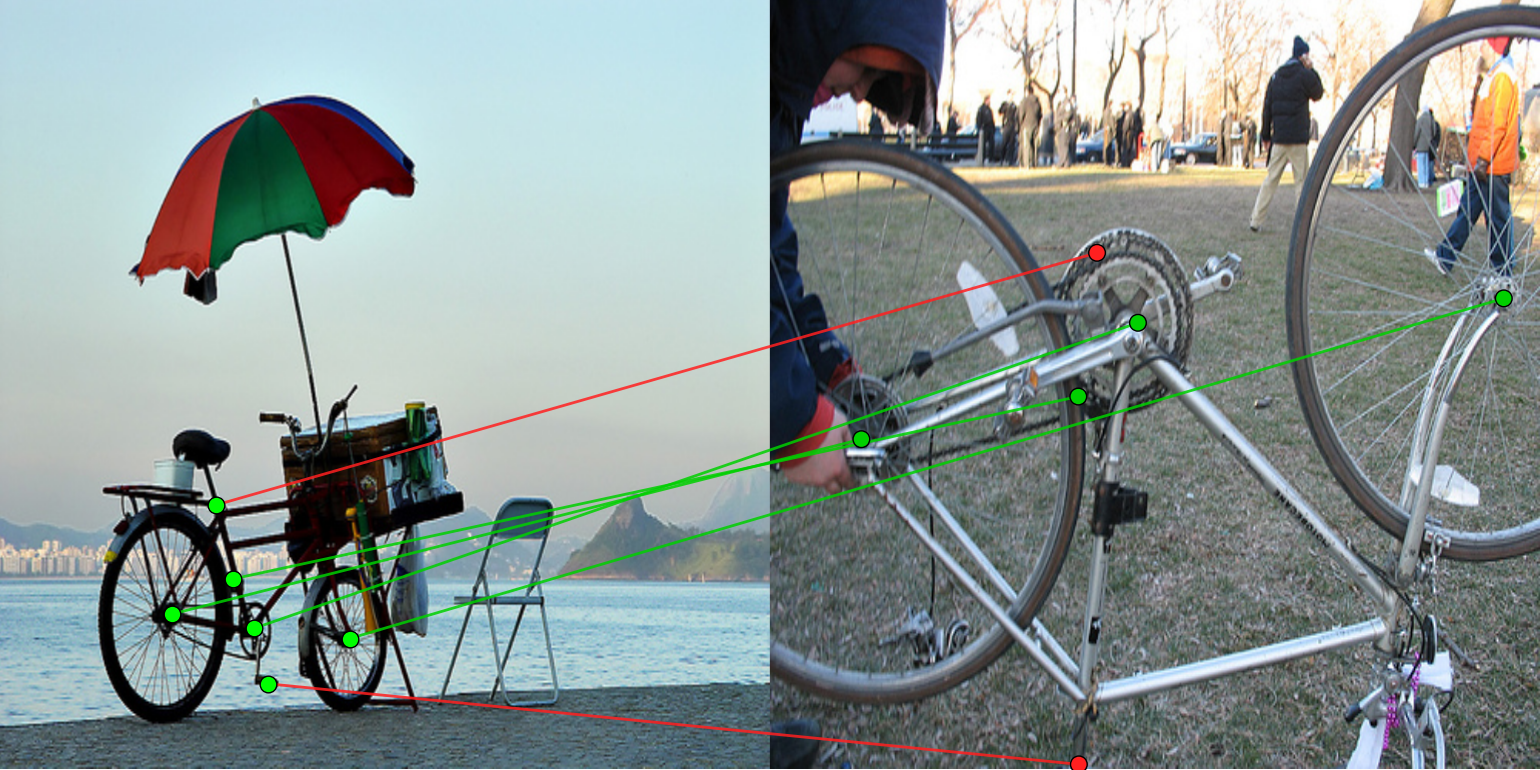
\includegraphics[width=0.48\textwidth]{figures/qualitative/marco/match_ours_bicycle.png} \\
% \end{tabular}
% \caption{\textbf{Qualitative SPair-71k \cite{min2019spair71k} results for MARCO \cite{cuttano2026marco}.}
% Each image shows a source--target pair with predicted correspondences. We compare MARCO trained on SPair-71k against MARCO pretrained on our generated correspondences and then fine-tuned on SPair-71k.}
% \label{fig:qual_marco}
% \end{figure*}


% \begin{figure*}[t]
% \centering
% \setlength{\tabcolsep}{3pt}
% \begin{tabular}{cc}
% \textbf{GeoAware-SC Real-only} & \textbf{GeoAware-SC Ours P.T.$\rightarrow$Real} \\
% 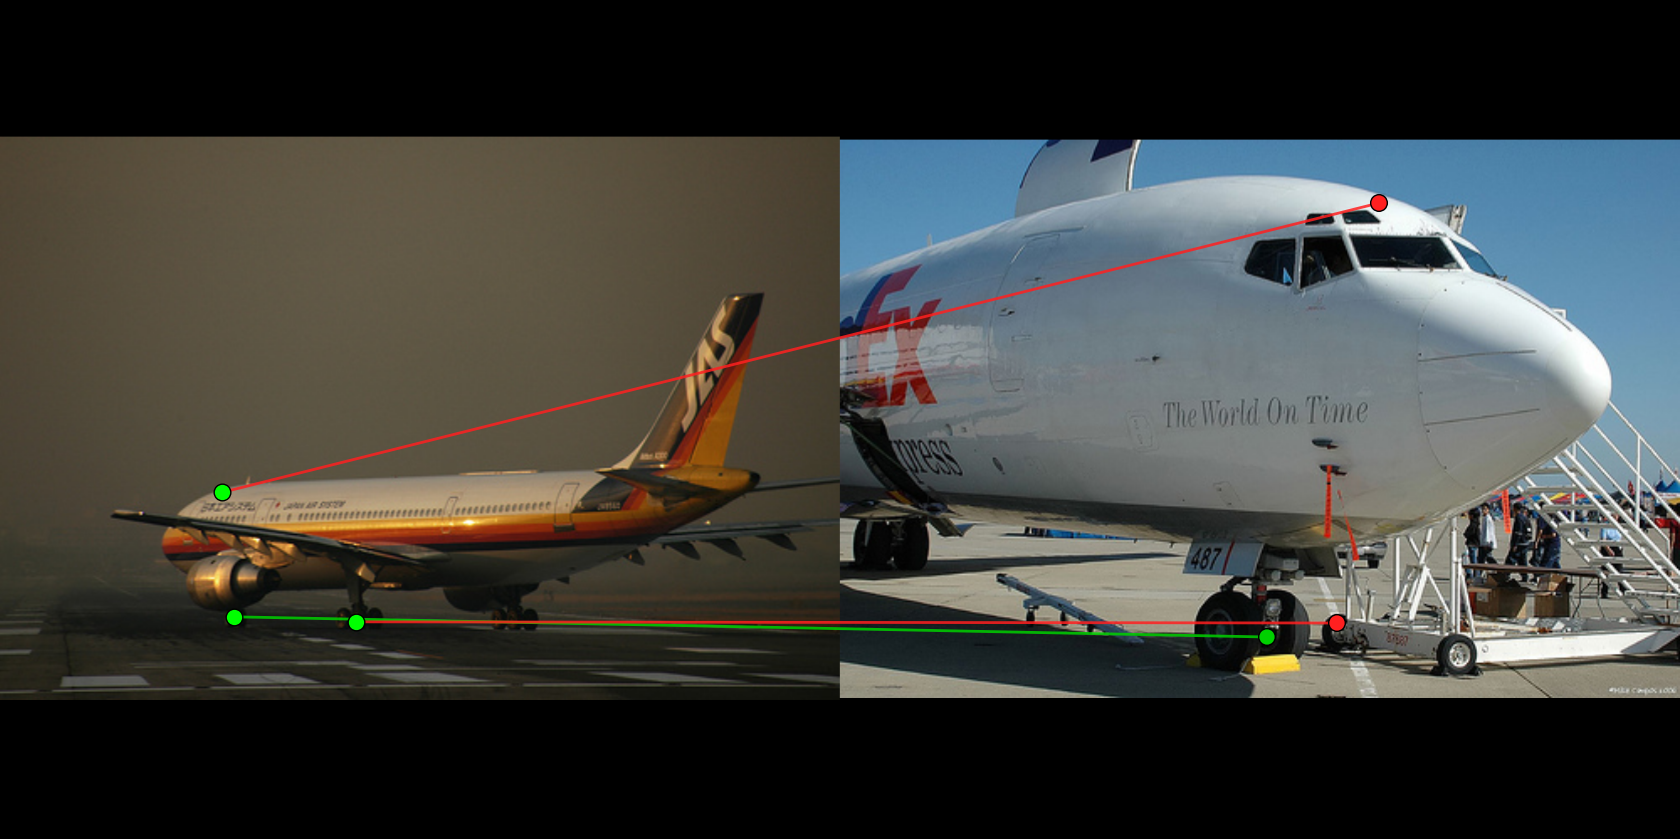
\includegraphics[width=0.48\textwidth]{figures/qualitative/geoaware/match_real_airplane.png} &
% 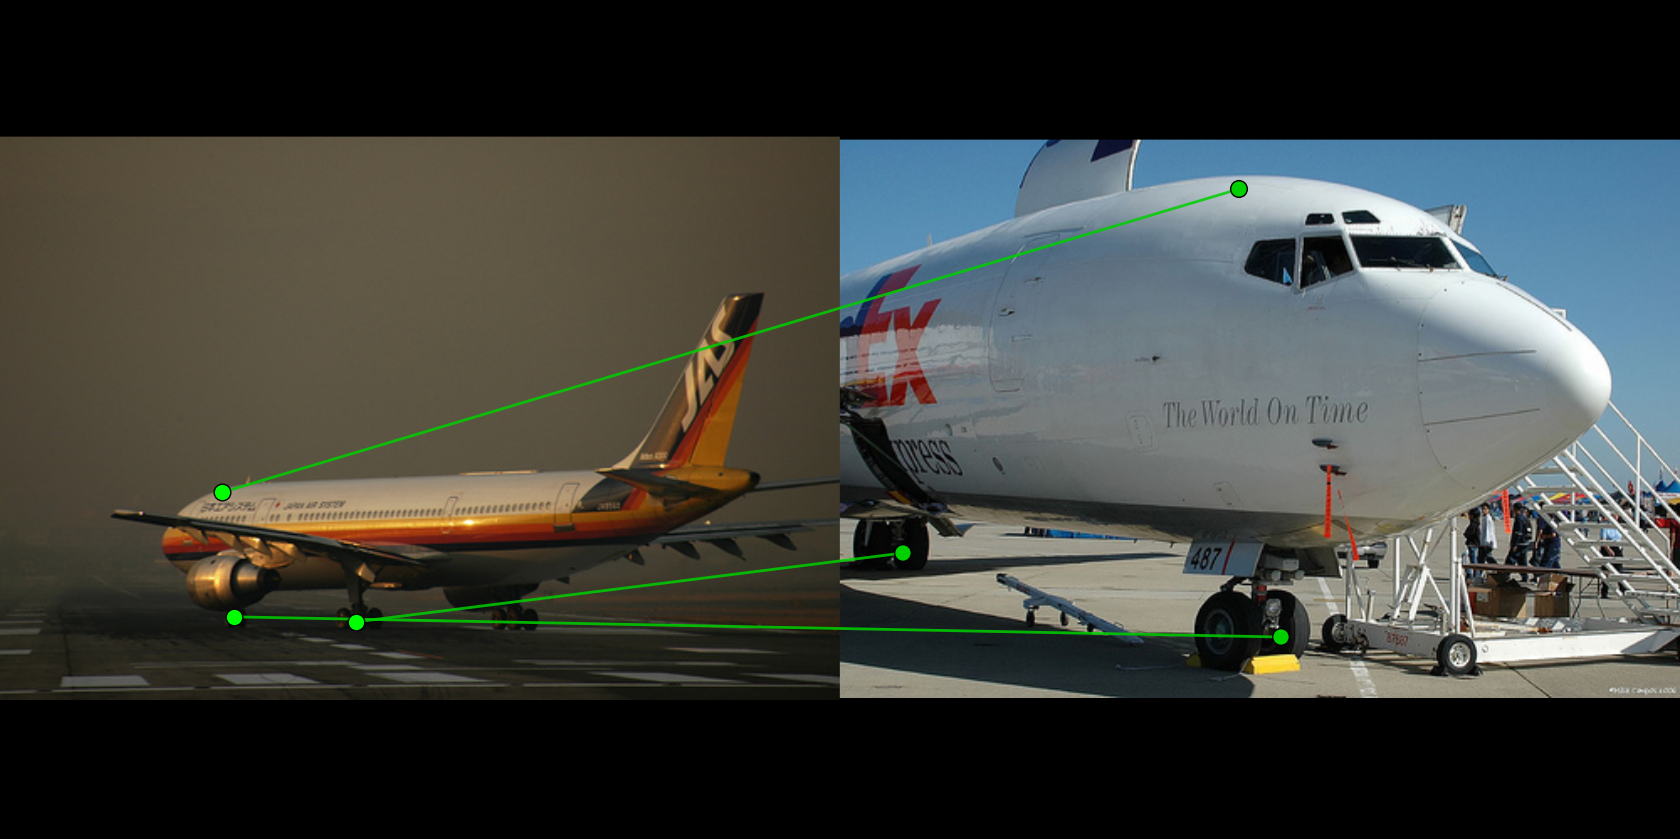
\includegraphics[width=0.48\textwidth]{figures/qualitative/geoaware/match_ours_airplane.png} \\
% 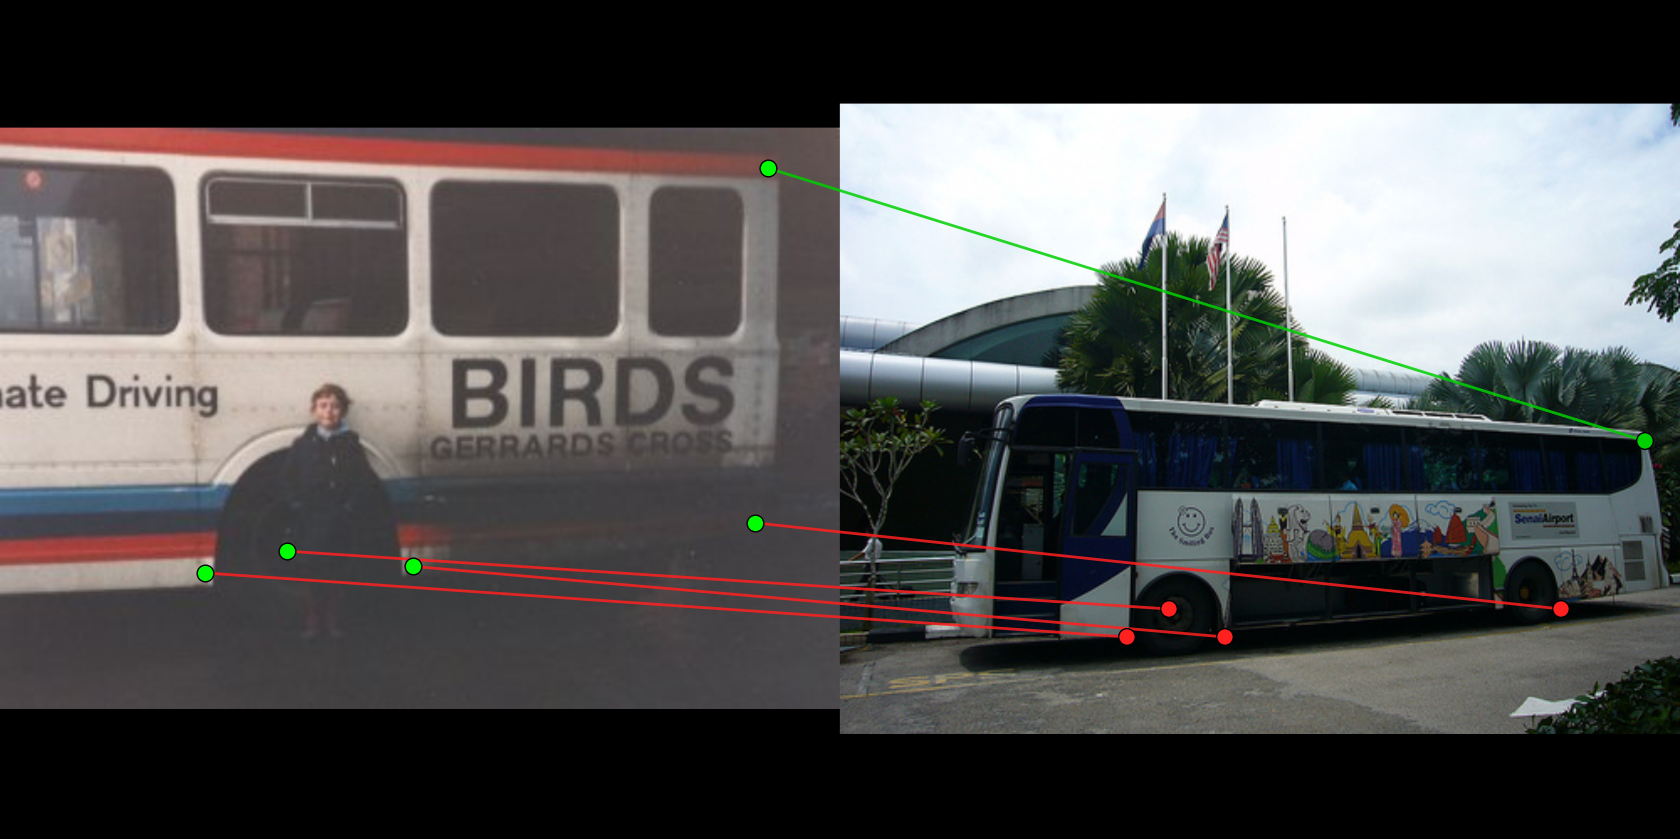
\includegraphics[width=0.48\textwidth]{figures/qualitative/geoaware/match_real_bus.png} &
% 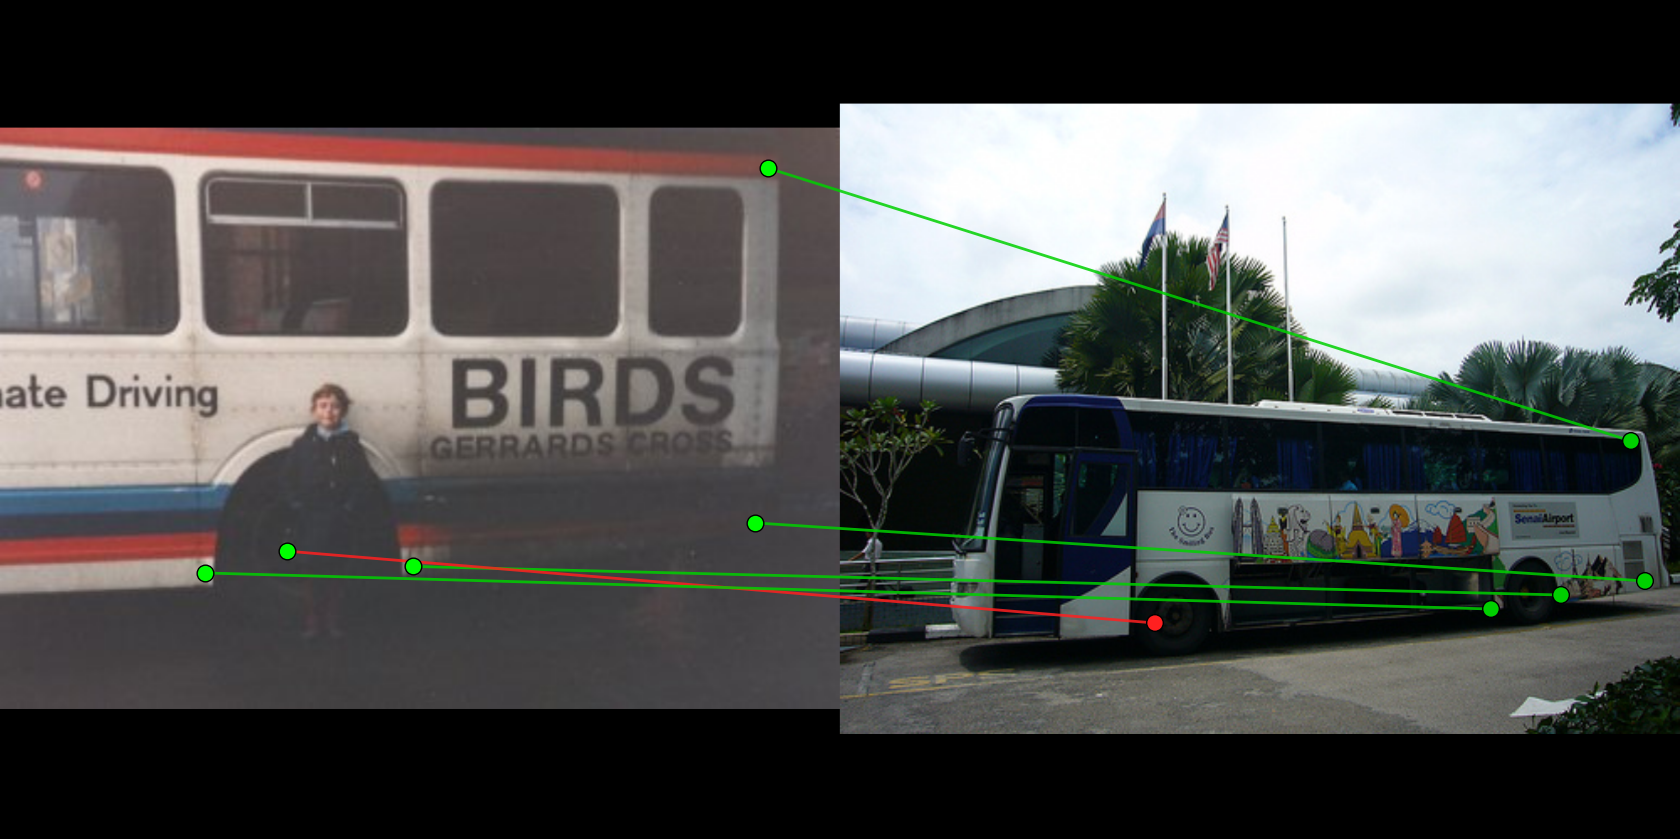
\includegraphics[width=0.48\textwidth]{figures/qualitative/geoaware/match_ours_bus.png} \\
% 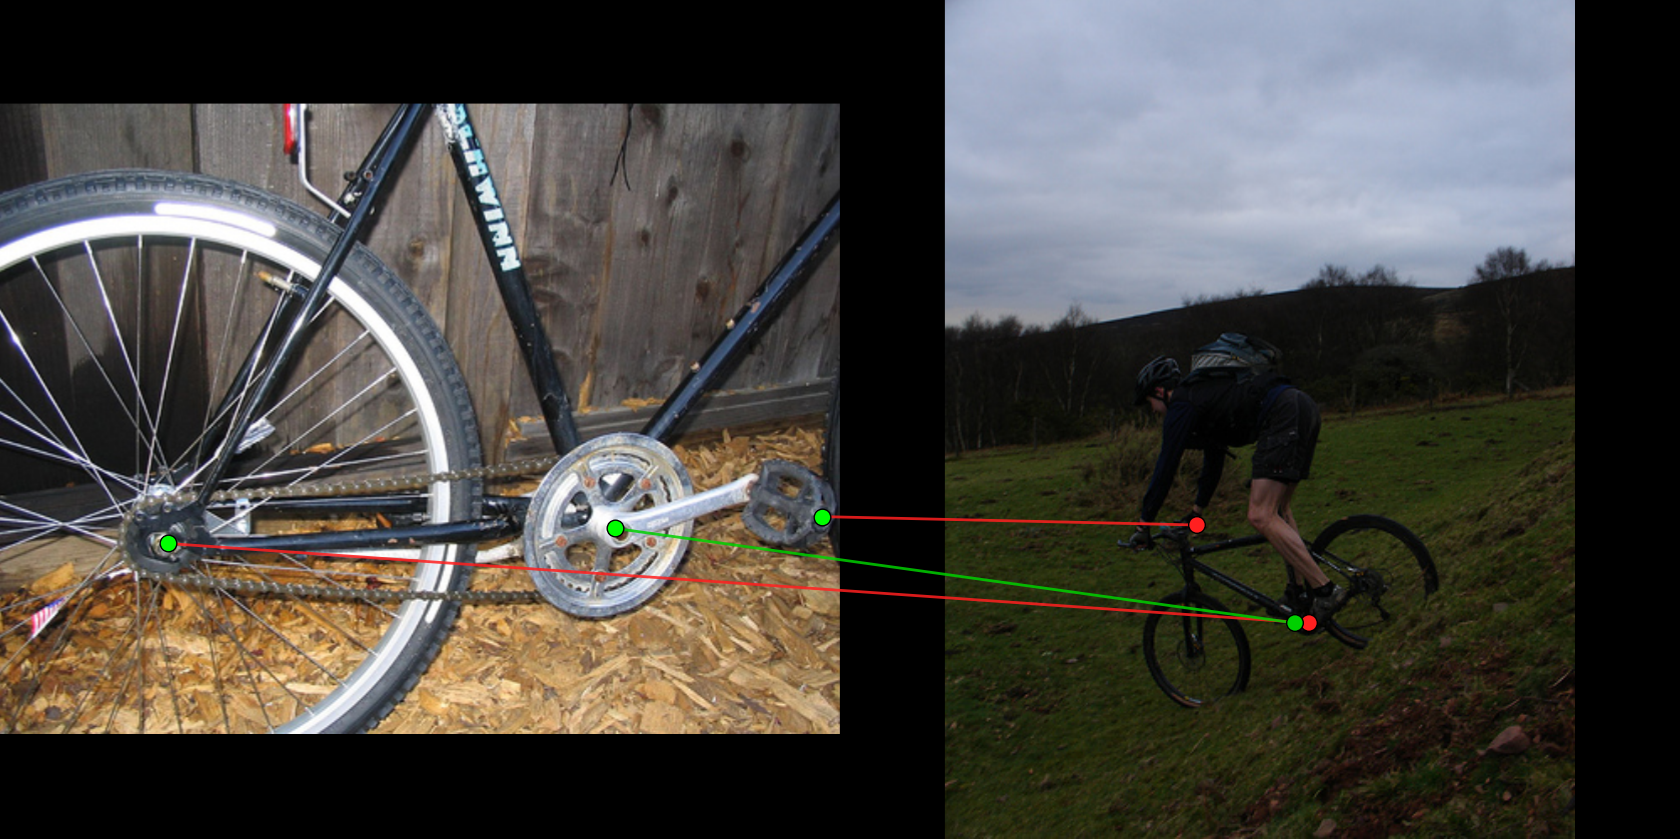
\includegraphics[width=0.48\textwidth]{figures/qualitative/geoaware/match_real_bike.png} &
% 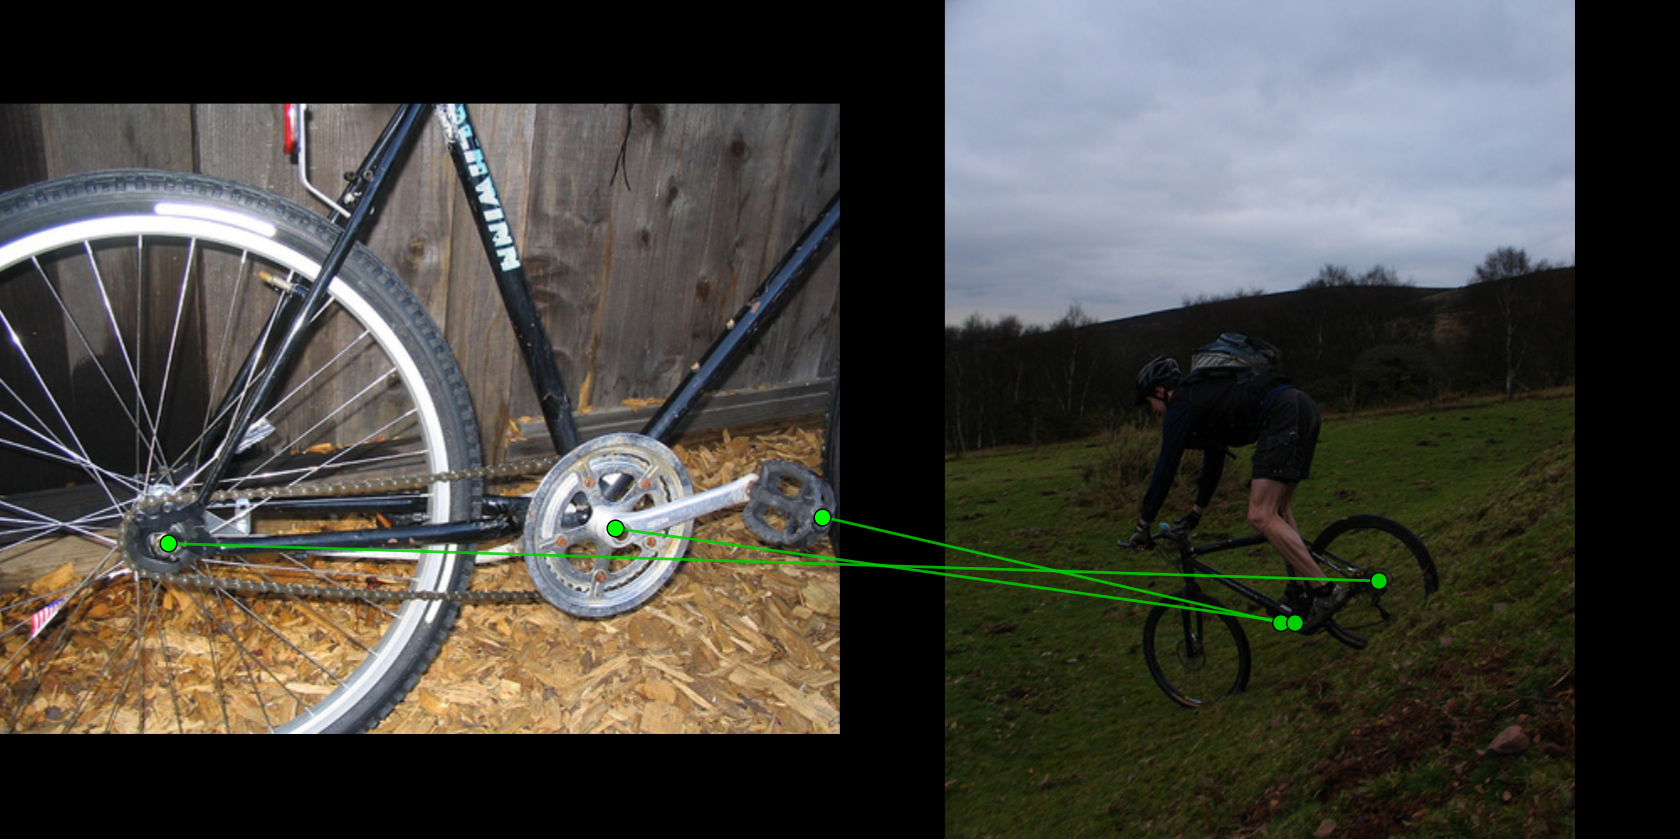
\includegraphics[width=0.48\textwidth]{figures/qualitative/geoaware/match_ours_bike.png} \\
% \end{tabular}
% \caption{\textbf{Qualitative SPair-71k \cite{min2019spair71k} results for GeoAware-SC \cite{zhang2024tellingLeftFromRight}.}
% Each image shows a source--target pair with predicted correspondences. We compare GeoAware-SC trained on SPair-71k against GeoAware-SC pretrained on our generated correspondences and then fine-tuned on SPair-71k.}
% \label{fig:qual_geoaware}
% \end{figure*}


\clearpage
\subsection{Qualitative Results on KeypointNet}

We provide qualitative correspondence results on KeypointNet \cite{you2020}, comparing our predicted correspondences against sparse human-annotated semantic keypoints. For each object pair, we use the human-annotated keypoints on the source object as queries and predict the corresponding points on the target object. As shown in \autoref{fig:keypointnet_examples}, our predictions generally align well with the human annotations across different categories. Predicted correspondences are shown in lighter colors, while the human annotations are shown in darker colors. Red lines connect each prediction to its corresponding ground-truth annotation.

We further show examples with strong agreement in \autoref{fig:keypointnet_strong_overlap}. The close overlap between our predictions and the human annotations indicates that our generated correspondences are highly consistent with the sparse semantic keypoints used for evaluation.

\begin{figure}[h]
    \centering

    \begin{subfigure}[b]{0.48\linewidth}
        \centering
        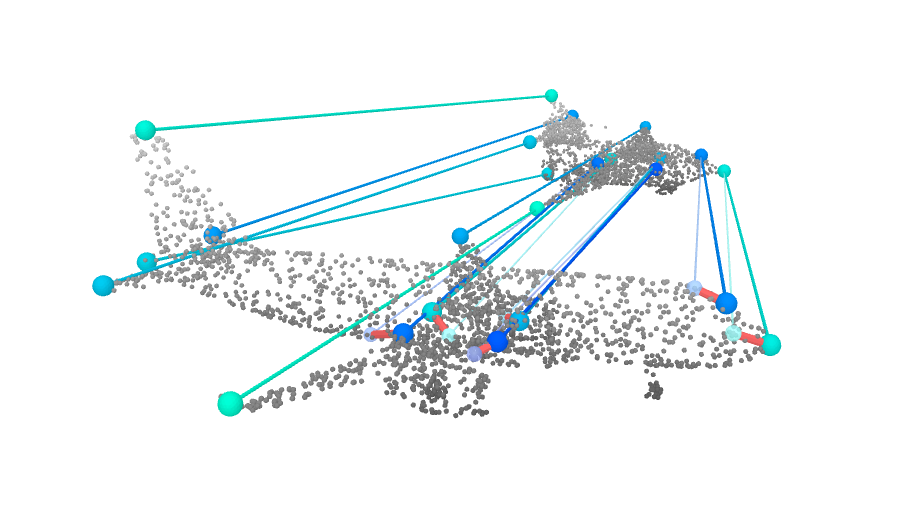
\includegraphics[width=\linewidth]{sup_mat/figures/airplane_top15_464a8718_x_dfa36bff_yaw-253p84_pitch76p57.png}
        \caption{Airplanes}
        \label{fig:example_a}
    \end{subfigure}
    \hfill
    \begin{subfigure}[b]{0.48\linewidth}
        \centering
        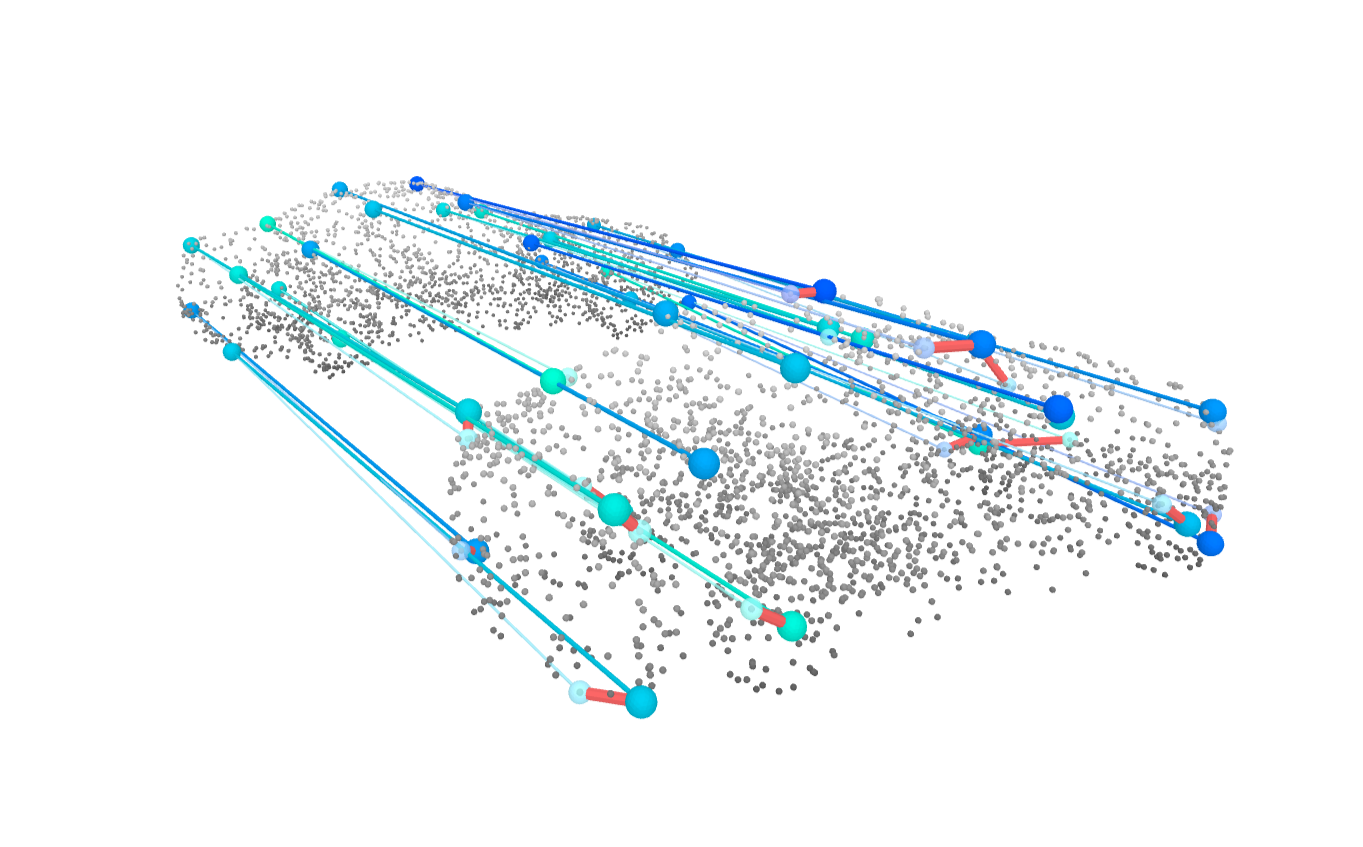
\includegraphics[width=\linewidth]{sup_mat/figures/car_top02_119033fe_x_1836f75b_yaw-298p07_pitch74p22.png}
        \caption{Cars}
        \label{fig:example_b}
    \end{subfigure}

    \caption{\textbf{Qualitative correspondence results on KeypointNet \cite{you2020}}
    We compare our predicted correspondences with human-annotated keypoints on the target object. Predicted correspondences are shown in lighter colors, while human annotations are shown in darker colors. Red lines connect each prediction to its corresponding ground-truth annotation, visualizing the localization difference between them.}
    \label{fig:keypointnet_examples}
\end{figure}

\begin{figure}[h]
    \centering

    \begin{subfigure}[b]{0.45\linewidth}
        \centering
        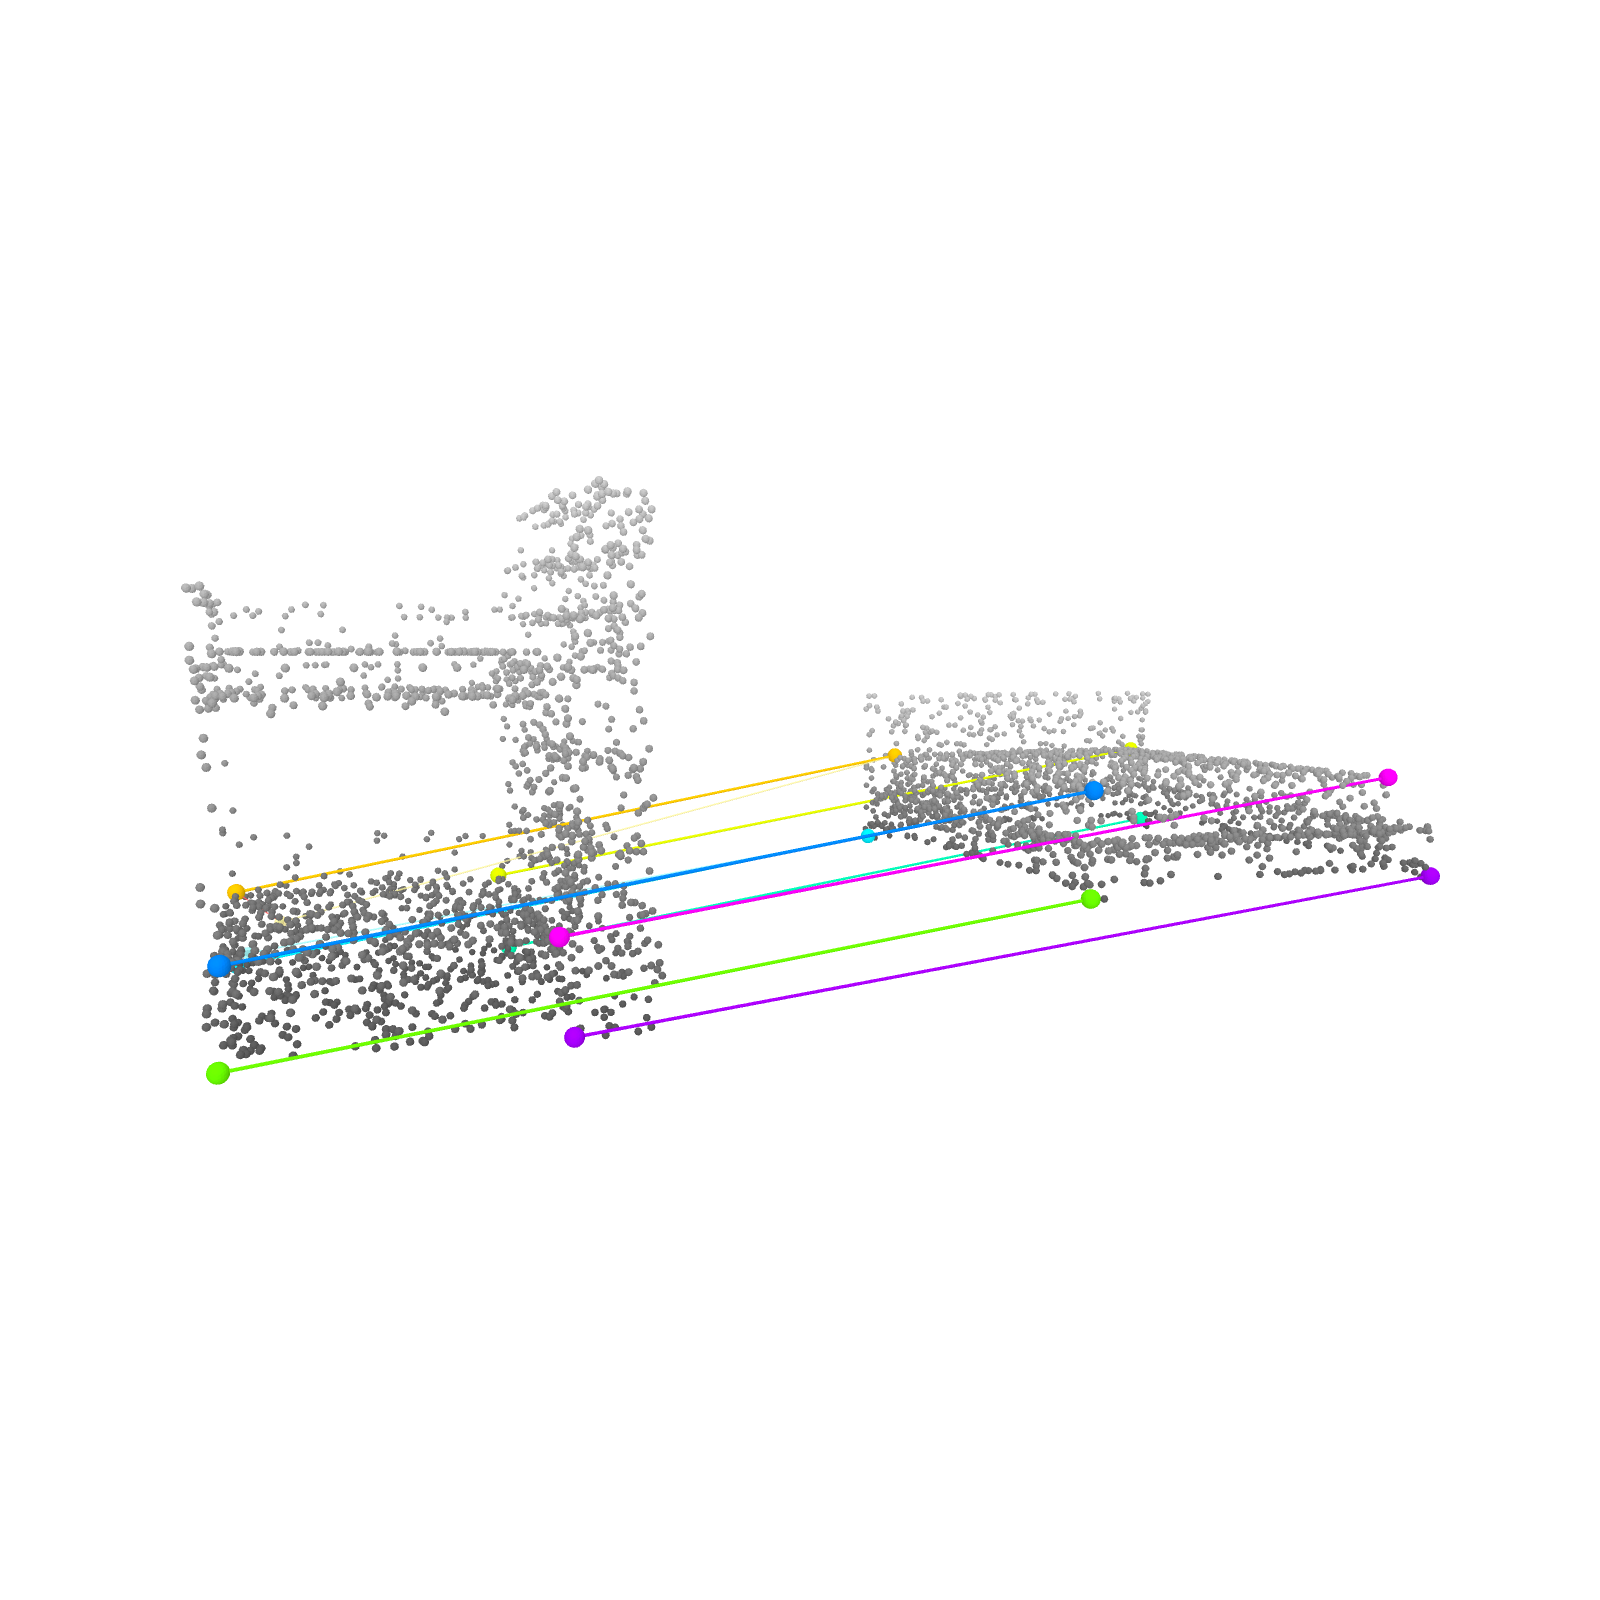
\includegraphics[trim={10 350 10 400},clip,width=\linewidth,height=\linewidth,keepaspectratio]{sup_mat/figures/bed_top11_ac97ffc6_x_e2532c6b_yaw-200p22_pitch84p01.png}
        \caption{Bed}
        \label{fig:square_bed}
    \end{subfigure}
    \hfill
    \begin{subfigure}[b]{0.45\linewidth}
        \centering
        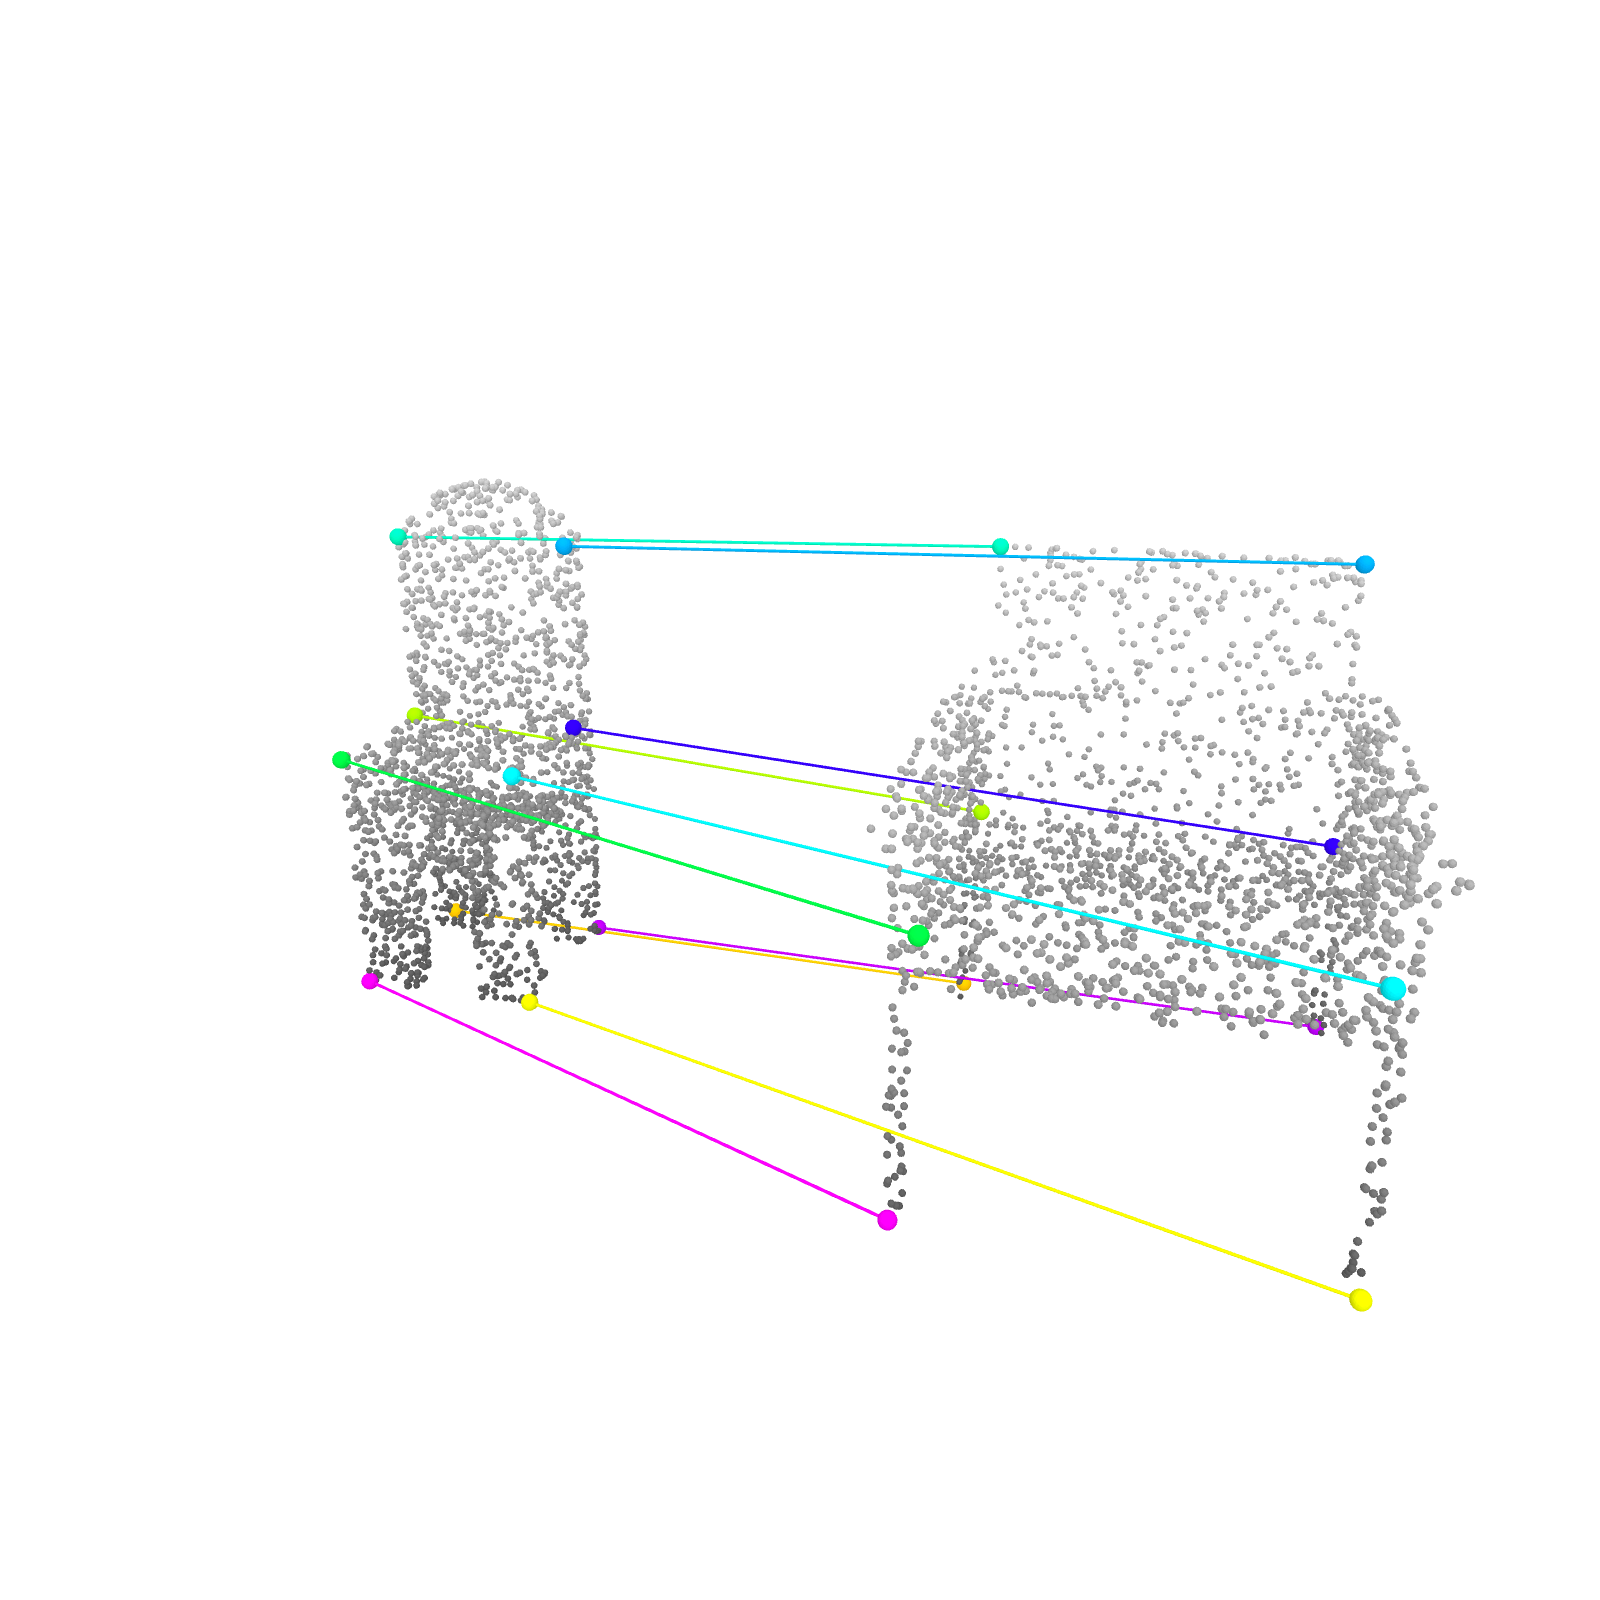
\includegraphics[trim={10 150 10 400},clip,width=\linewidth,height=\linewidth,keepaspectratio]{sup_mat/figures/chair_top11_2828b98d_x_4647b2b9_yaw-164p94_pitch69p52.png}
        \caption{Chair}
        \label{fig:square_chair}
    \end{subfigure}

    \begin{subfigure}[b]{0.45\linewidth}
        \centering
        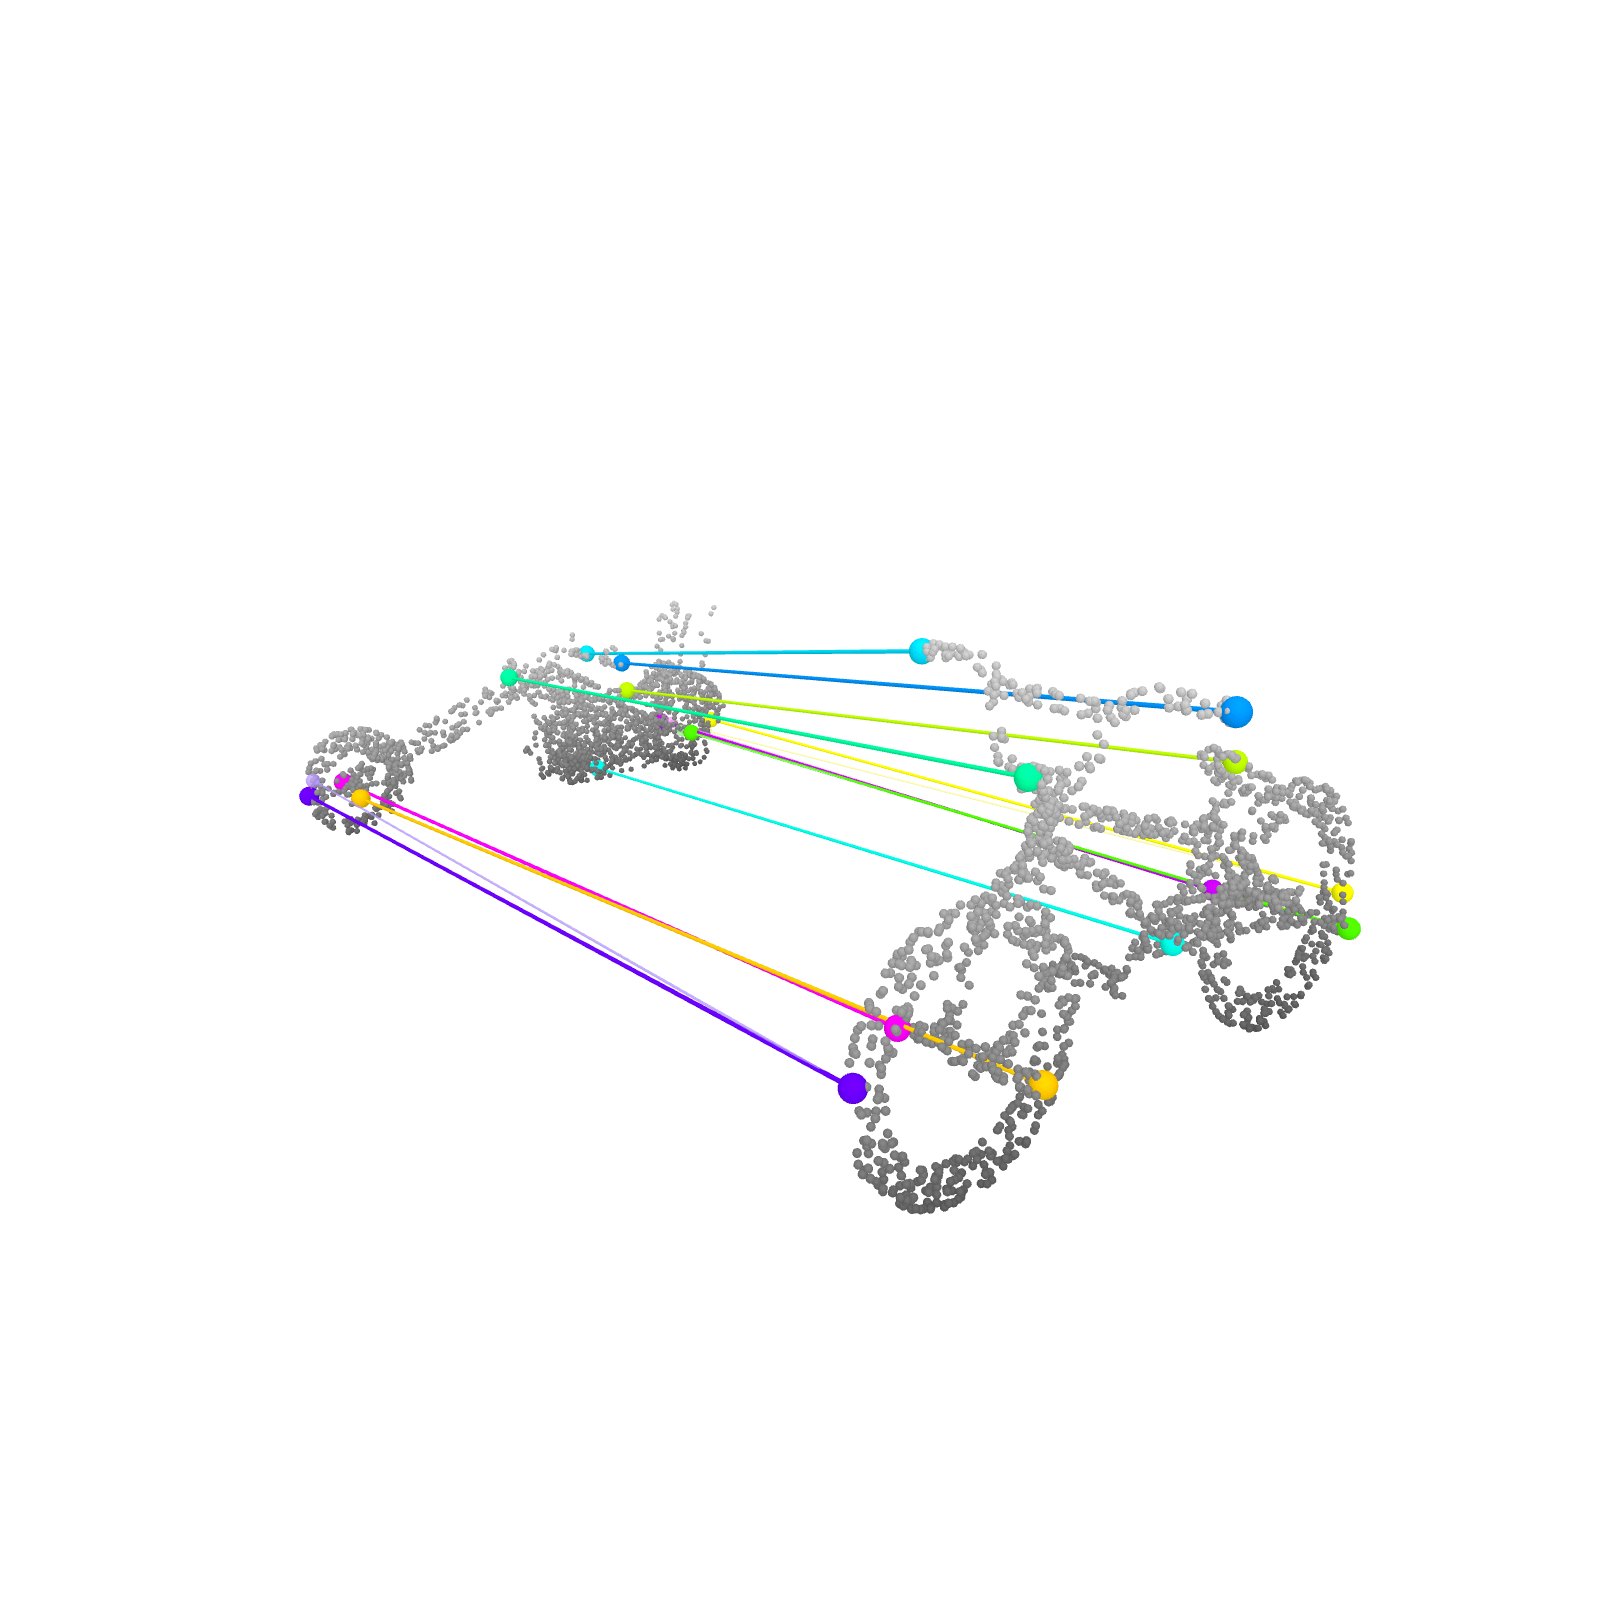
\includegraphics[trim={10 350 10 400},clip,width=\linewidth,height=\linewidth,keepaspectratio]{sup_mat/figures/motorcycle_top03_1d8fb258_x_a1553e0b_yaw-131p95_pitch72p26.png}
        \caption{Motorcycle}
        \label{fig:square_motorcycle}
    \end{subfigure}
    \begin{subfigure}[b]{0.45\linewidth}
        \centering
        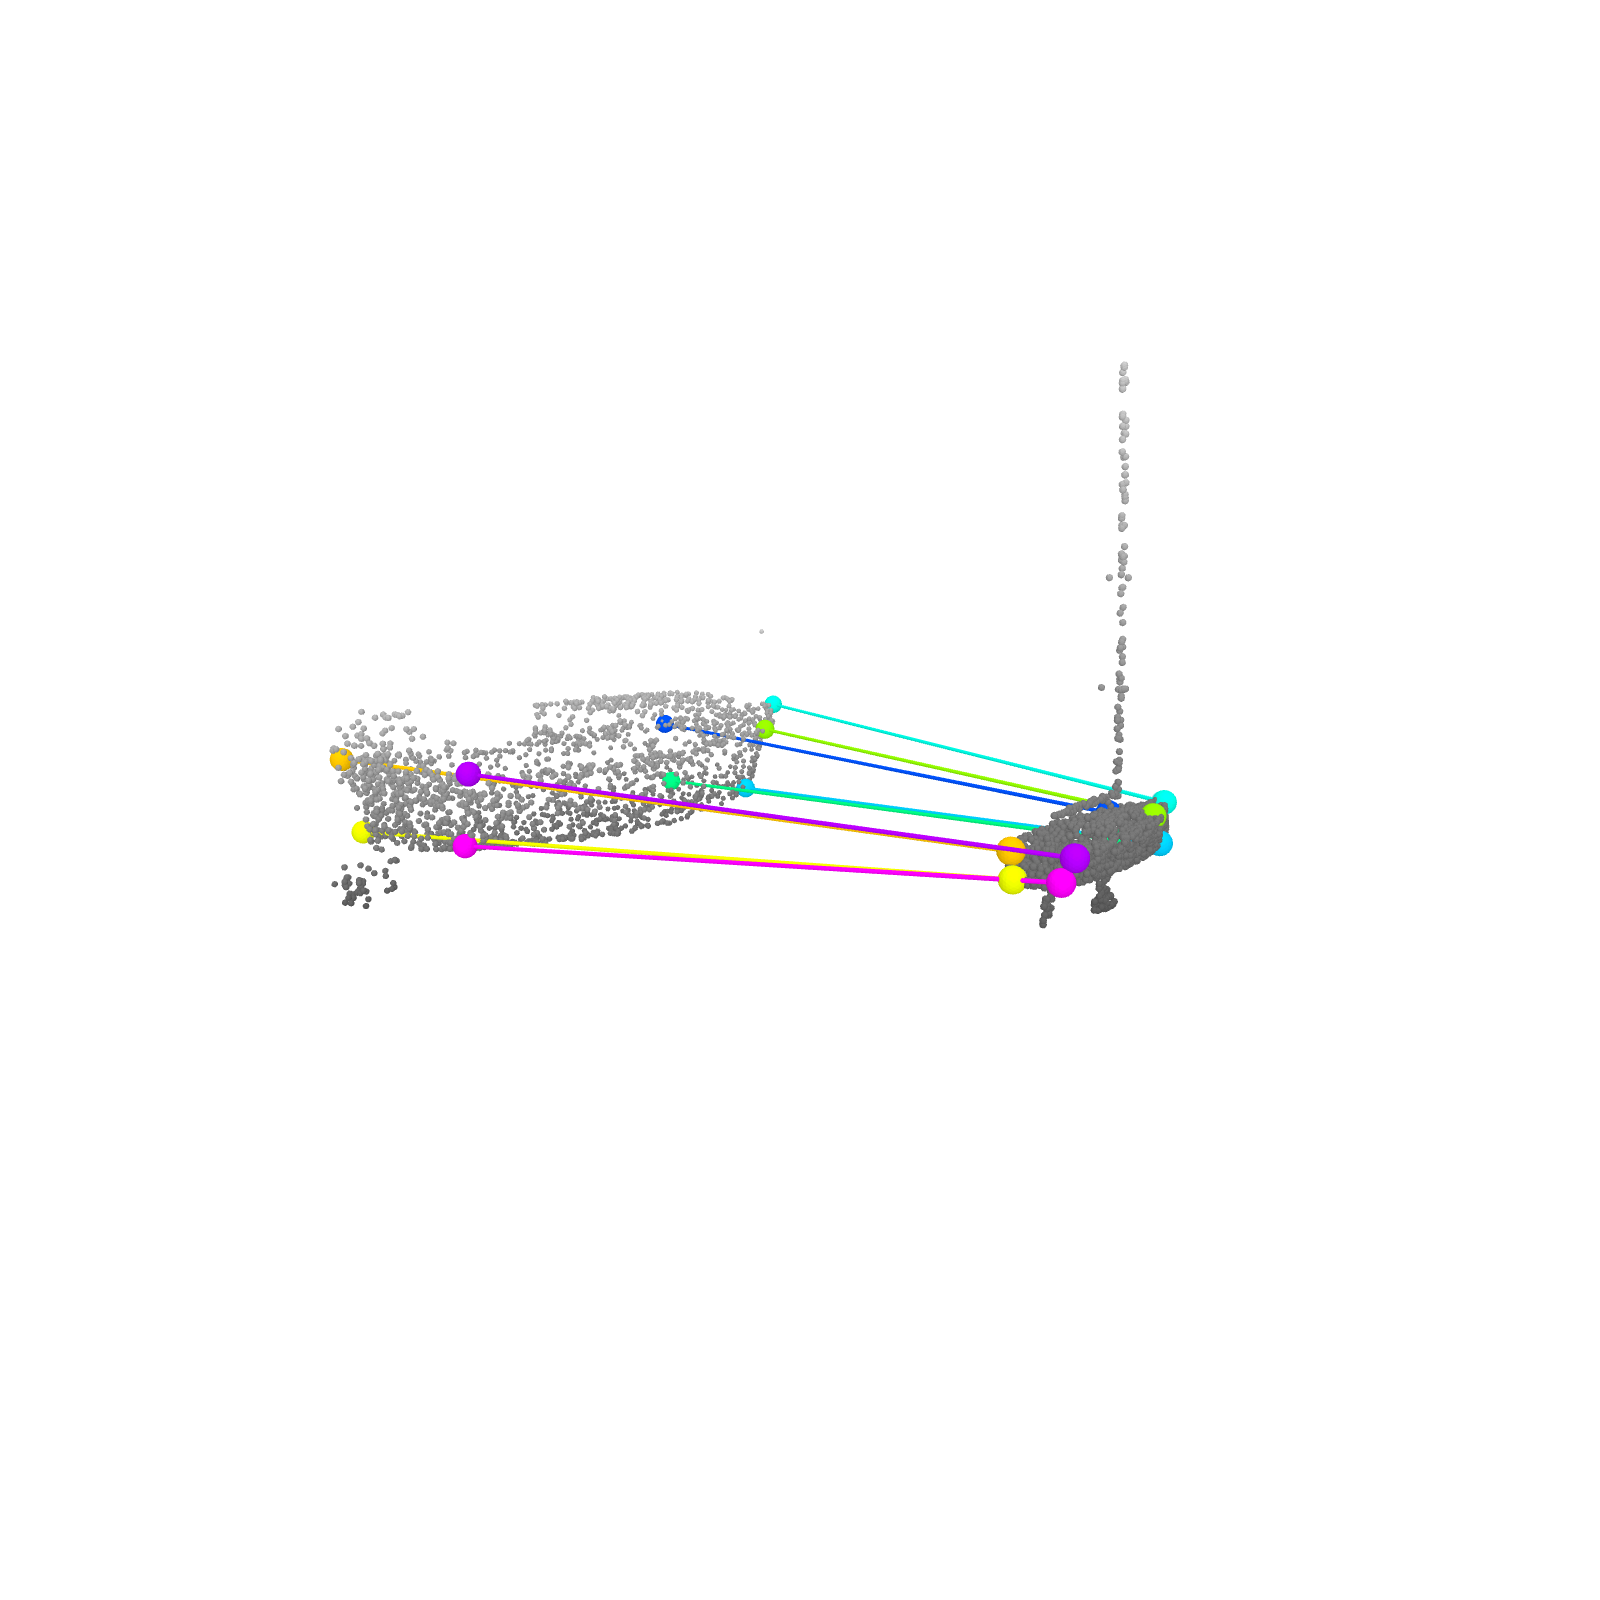
\includegraphics[trim={10 550 10 400},clip,width=\linewidth,height=\linewidth,keepaspectratio]{sup_mat/figures/vessel_top02_cc6656ba_x_e604463b_yaw-325p50_pitch80p49.png}
        \caption{Vessel}
        \label{fig:square_vessel}
    \end{subfigure}

    \caption{\textbf{KeypointNet \cite{you2020} examples with strong annotation agreement.}
    Predicted correspondences are shown in lighter colors, while human annotations are shown in darker colors. The strong overlap between the two indicates that our pipeline recovers correspondences that are highly consistent with human semantic annotations.}
    \label{fig:keypointnet_strong_overlap}
\end{figure}









\clearpage
\section{Additional Quantitative Results on SPair-71k}
\label{sup:supp_spair}

We provide additional evaluation results on SPair-71k \cite{min2019spair71k} across multiple PCK thresholds and training regimes. While the main paper reports PCK@0.10 (see \autoref{tab:spair_pck010}), here we analyze performance at stricter and looser thresholds, and compare four training strategies: \emph{Synth-only}, \emph{Both} (joint real and synthetic training), \emph{Real-only}, and \emph{Synth$\rightarrow$Real} (pretraining on synthetic correspondences followed by fine-tuning on real data).

\paragraph{MARCO \cite{cuttano2026marco} results.}
Across all thresholds (PCK@0.01-0.20), the Synth$\rightarrow$Real setting consistently outperforms Real-only training at practical thresholds. In particular, improvements of $+2.4$ to $+2.9$ PCK are observed for PCK@0.05--0.20. At PCK@0.10, performance improves from $86.39$ to $89.28$, matching the results reported in \autoref{tab:spair_pck010}.

At very strict thresholds (PCK@0.01), Synth$\rightarrow$Real slightly underperforms Real-only ($-2.17$). However, this gap disappears at more relaxed thresholds, where Synth$\rightarrow$Real consistently achieves the best performance.

We also observe that joint training (\emph{Both}) underperforms Real-only, indicating that naive mixing of synthetic and real data is suboptimal, and that a two-stage training strategy is more effective.

\paragraph{GeoAware-SC \cite{zhang2024tellingLeftFromRight} results.}
We observe the same qualitative trend for GeoAware-SC. Synth$\rightarrow$Real consistently improves over Real-only training across all evaluated thresholds, while Synth-only performs poorly in isolation. Joint training again underperforms Real-only, reinforcing that synthetic correspondences are most effective as a pretraining signal rather than as direct supervision.

At PCK@0.10, as we see in the results from the main paper (\autoref{tab:spair_pck010}), synthetic pretraining improves performance from $79.36$ to $83.73$, corresponding to a gain of $+4.37$ PCK.

\paragraph{Cross-architecture consistency.}
Using the PCK@0.10 results from \autoref{tab:spair_pck010}, we observe consistent improvements across architectures and feature choices:
\begin{center}
\begin{tabular}{lccccc}
\toprule
Architecture & DINOv2 \cite{oquab2024dinov2} & Stable Diffusion \cite{rombach2022stablediffusion} & Real-only & Synth$\rightarrow$Real & Gain \\
\midrule
GeoAware-SC \cite{zhang2024tellingLeftFromRight} & \checkmark & \checkmark & 79.36 & 83.73 & +4.37 \\
MARCO \cite{cuttano2026marco}      & \checkmark & $\times$ & 86.39 & 89.28 & +2.89 \\
\bottomrule
\end{tabular}
\end{center}

GeoAware-SC \cite{zhang2024tellingLeftFromRight} uses both DINOv2 \cite{oquab2024dinov2} and Stable Diffusion \cite{rombach2022stablediffusion} features, while MARCO \cite{cuttano2026marco} relies on DINOv2 features without Stable Diffusion. The gains across both settings suggest that our synthetic pretraining signal is not tied to a specific feature family, but provides useful semantic-geometric supervision across different recent correspondence models.

These consistent gains suggest that the benefit of synthetic pretraining is largely architecture-agnostic. Rather than improving a specific model design, the generated correspondences provide a strong pretraining signal that improves representation quality across different backbones and matching heads.

\paragraph{Summary.}
Overall, these results support three key observations: (i) synthetic correspondences alone are insufficient for high performance, (ii) naive joint training is suboptimal, and (iii) a two-stage Synth$\rightarrow$Real strategy consistently yields the best results. This pattern holds across architectures and evaluation thresholds, reinforcing the generality of the proposed data generation pipeline.

% Add your qualitative figures / tables here
% Example:
% \subimport{./sup_mat/figures}{qualitative_results}
% \subimport{./sup_mat/figures}{more_spair_vis}
% \subimport{./sup_mat/figures}{more_keypointnet_vis}
\clearpage
\section{Extended Ablation Study}
\label{sup:ablation_study}
\subsection{Registration Method Ablation}
\label{sup:ablation_registration}

We ablate the deformation model used in the registration stage prior to correspondence extraction. All other components are kept fixed, including lifted DINOv2 \cite{oquab2024dinov2} features, nearest-neighbor assignment, and the semantic threshold $\tau_{\mathrm{sem}}=0.85$. We compare our default continuous piecewise-affine (CPA) model with two alternatives: a global affine transformation and a thin-plate spline (TPS) deformation.

\paragraph{Affine.}
As a global transformation baseline, we use an affine transformation

\[
f(\mathbf{x}) = \mathbf{A}\mathbf{x} + \mathbf{t},
\]
where $\mathbf{A} \in \mathbb{R}^{3\times 3}$ and $\mathbf{t} \in \mathbb{R}^{3}$. This model has 12 learnable parameters and is optimized with Adam using the same Chamfer objective. Since it cannot model non-rigid variation, it serves as a baseline for how much alignment can be explained by global pose normalization alone.

\paragraph{Continuous Piecewise-Affine (CPA).}
Our default model uses a $6 \times 6 \times 6$ control grid (216 vertices) over the normalized 3D domain, tetrahedralized via Delaunay triangulation. Each vertex has a learnable displacement, and each point is warped using barycentric interpolation within its enclosing tetrahedron. This yields a deformation that is locally affine and globally continuous. We enforce smoothness by penalizing squared differences between neighboring vertex displacements, with $\lambda_{\mathrm{smooth}}=0.3$. The model has 648 degrees of freedom.

\paragraph{Thin-Plate Spline (TPS).}
We compare with a classical smooth non-rigid deformation
\[
f(\mathbf{x}) = \mathbf{a} + \mathbf{B}\mathbf{x}
+ \sum_{k=1}^{K} \mathbf{w}_k \, U(\|\mathbf{x}-\mathbf{c}_k\|),
\qquad U(r) = -r,
\]
where $\mathbf{B}\in\mathbb{R}^{3\times3}$, $\mathbf{a}\in\mathbb{R}^{3}$, and $\mathbf{w}_k\in\mathbb{R}^{3}$. We use $K=216$ control points sampled from the source, resulting in a similar number of parameters to CPA (660 vs.\ 648). Smoothness is enforced with an $\ell_2$ penalty on the radial weights.

\paragraph{Protocol.}
We evaluate all three methods on the 16 KeypointNet \cite{you2020} categories. For each category, we sample 100 source-target pairs from random instances and run all methods on them. All hyperparameters are shared: 10,000 Adam iterations with early stopping on a loss plateau, a learning rate of $0.005$, and no pair-level filtering. Performance is measured using PCK at multiple thresholds, where a prediction is correct if it falls within $\tau \cdot d$ of the ground-truth target keypoint, with $d$ the target bounding-box diagonal.

\paragraph{Results.}
\autoref{tab:ablation_registration} reports mean PCK across all categories. CPA achieves the best average performance at four of the five PCK thresholds, while TPS is slightly better only at PCK@0.05. Overall, CPA and TPS obtain very similar accuracy, indicating that the choice of non-rigid basis has limited impact on correspondence quality.

\begin{table}[h!]
\centering
\small
\caption{\textbf{Registration ablation on KeypointNet.}
Mean PCK across all 16 categories. PCK thresholds define the allowed normalized distance from the ground-truth keypoint, measured as a fraction of the target bounding-box diagonal. DOF denotes the number of learnable parameters. Time reports the mean registration time per pair on a single A6000 GPU. Best results are shown in \textbf{bold}.}
\label{tab:ablation_registration}
\setlength{\tabcolsep}{4pt}
\begin{tabular}{lccccccc}
\toprule
Method & DOF & Time (s/pair) & PCK@0.01 & PCK@0.05 & PCK@0.10 & PCK@0.15 & PCK@0.20 \\
\midrule
Affine            & 12  & 1.15 & 0.221 & 0.686 & 0.898 & 0.960 & 0.982 \\
TPS ($K\!=\!216$) & 660 & 3.71 & 0.226 & \textbf{0.739} & 0.919 & 0.966 & 0.983 \\
CPA (ours)        & 648 & \textbf{1.13} & \textbf{0.236} & 0.729 & \textbf{0.922} & \textbf{0.971} & \textbf{0.986} \\
\bottomrule
\end{tabular}
\end{table}

In contrast, CPA is substantially more efficient. It is about $3.3\times$ faster per pair (1.13s vs.\ 3.71s), despite having a similar number of parameters. We also observe that CPA typically converges earlier. This difference arises from the underlying structure: CPA uses local barycentric interpolation within tetrahedra, while TPS requires dense kernel interactions between all points and control points at each iteration.

Compared with the affine baseline, CPA provides clear gains, especially at tighter PCK thresholds, highlighting the importance of non-rigid alignment for cross-instance correspondence.

\paragraph{Conclusion.}
This ablation supports two conclusions: (i) non-rigid deformation is essential for accurate alignment, as affine transformations perform significantly worse; and (ii) among non-rigid models, CPA offers a better accuracy-efficiency tradeoff, achieving similar performance to TPS while being significantly faster and more stable in practice.

\subsection{Ablation on Semantic Filtering}
\label{sup:ablation_semantic_filtering}

We analyze the role of semantic filtering in our pipeline. Specifically, we study (i) the effect of removing semantic filtering entirely, (ii) the contribution of correspondence-level filtering alone, and (iii) the impact of the correspondence-level semantic threshold $\tau_{\mathrm{sem}}$ when combined with pair-level filtering. All experiments are conducted on KeypointNet using the same evaluation protocol as in the main paper.

\subsubsection{No Semantic Filtering}
\label{sup:no_semantic_filtering}

We first evaluate the pipeline without any semantic filtering. In this setting, all object pairs are retained, and correspondences are obtained directly from CPA registration followed by nearest-neighbor assignment.

\autoref{tab:unfiltered} shows that this setting produces significantly lower accuracy. While geometric alignment alone can recover many plausible correspondences, it frequently matches inconsistent regions across instances, leading to degraded PCK, especially at stricter thresholds (e.g., PCK@0.05 and PCK@0.10). This highlights the limitation of relying solely on geometry for cross-instance correspondence and the need for a semantic pruning step.

\subimport{./sup_mat/tables}{unfiltered_keypointnet}

\subsubsection{Correspondence-Level Semantic Filtering Only}
\label{sup:only_corr_filtering}

We next evaluate correspondence-level semantic filtering alone, without pair-level filtering. In this setting, all object pairs are retained, and individual correspondences are pruned using a fixed threshold $\tau_{\mathrm{sem}}=0.85$.

\autoref{tab:pck_results} shows that this step alone leads to a substantial improvement over the no-filtering baseline. In particular, mean PCK@0.10 improves from 0.84 to 0.91, confirming that a large portion of the error arises from semantically inconsistent matches that are geometrically plausible but incorrect.

\subimport{./sup_mat/tables}{only_sem_fil_table}

\subsubsection{Correspondence-Level Semantic Threshold}
\label{sup:ablation_semantic_threshold_corr}

We finally analyze the effect of the semantic threshold $\tau_{\mathrm{sem}}$ when combined with pair-level filtering, as used in the full pipeline.

This threshold controls an accuracy-coverage tradeoff. A stricter threshold keeps fewer but more reliable matches, while a looser threshold retains more matches but allows more semantically inconsistent correspondences. To quantify coverage, we report the \emph{median GT-used rate} across categories. A ground-truth keypoint is counted as used if at least one surviving correspondence remains within $0.05$ of the object bounding-box diagonal from the ground-truth location.

Importantly, this metric is conservative. KeypointNet annotations are sparse and typically located on salient corners or extreme parts, while our method produces dense correspondences across the object surface (see Fig.~1). As a result, semantically valid correspondences that do not fall within the $0.05$ evaluation radius are still counted as missed.

\begin{table}[h!]
\centering
\small
\caption{\textbf{Ablation on the correspondence-level semantic threshold (with pair-level filtering).}
Results are averaged over three random seeds and 16 KeypointNet categories. Median GT-used rate denotes the median fraction across categories of ground-truth keypoints that remain evaluable after correspondence-level pruning.}
\label{tab:semantic_threshold_ablation}
\setlength{\tabcolsep}{5pt}
\begin{tabular}{lccccc}
\toprule
$\tau_{\mathrm{sem}}$ & PCK@0.05 $\uparrow$ & PCK@0.10 $\uparrow$ & PCK@0.15 $\uparrow$ & PCK@0.20 $\uparrow$ & Median GT-used rate $\uparrow$ \\
\midrule
0.50 & 0.758 & 0.930 & 0.974 & 0.988 & 0.260 \\
0.85 & 0.749 & 0.926 & 0.973 & 0.989 & 0.576 \\
1.50 & 0.699 & 0.896 & 0.960 & 0.983 & 0.915 \\
\bottomrule
\end{tabular}
\end{table}

\autoref{tab:semantic_threshold_ablation} shows that the choice of threshold controls a clear tradeoff between accuracy and coverage. A strict threshold ($\tau_{\mathrm{sem}}=0.5$) achieves the highest accuracy but retains only 26.0\% of ground-truth keypoints, while a loose threshold ($\tau_{\mathrm{sem}}=1.5$) retains 91.5\% but significantly degrades accuracy.

We therefore use $\tau_{\mathrm{sem}}=0.85$ as a practical middle point: it maintains similar accuracy to the stricter threshold while more than doubling the median GT-used rate (26.0\% $\rightarrow$ 57.6\%).

\paragraph{Discussion.}
Overall, these results show that semantic filtering is essential for removing geometrically plausible but semantically incorrect correspondences. Most of the improvement comes from correspondence-level filtering, while pair-level filtering provides an additional refinement by removing object pairs with insufficient semantic overlap.

\clearpage
\section{Qualitative Analysis of DINOv2 Based Semantic Filtering}
\label{sup:supp_semantic_analy}

We provide a qualitative analysis of the DINOv2 based semantic filtering used in our pipeline, both at the pair level and at the correspondence level. As shown in \autoref{fig:semantic_coverage_analysis}, we visualize the lifted DINOv2 features after joint PCA to three dimensions, and mark points according to whether they have any sufficiently similar semantic counterpart in the paired object. Green points have at least one point in the paired object with cosine similarity above our threshold of \(0.85\), while red points have no such candidate. We use this semantic coverage to filter object pairs that do not share enough semantic structure. In addition, for pairs that survive pair-level filtering, red points are guaranteed to be removed by our semantic pruning after registration. This filtering is complementary to the correspondence-level pruning, which further removes geometrically matched points whose assigned matches are semantically inconsistent.

\begin{figure}[h]
    \centering
    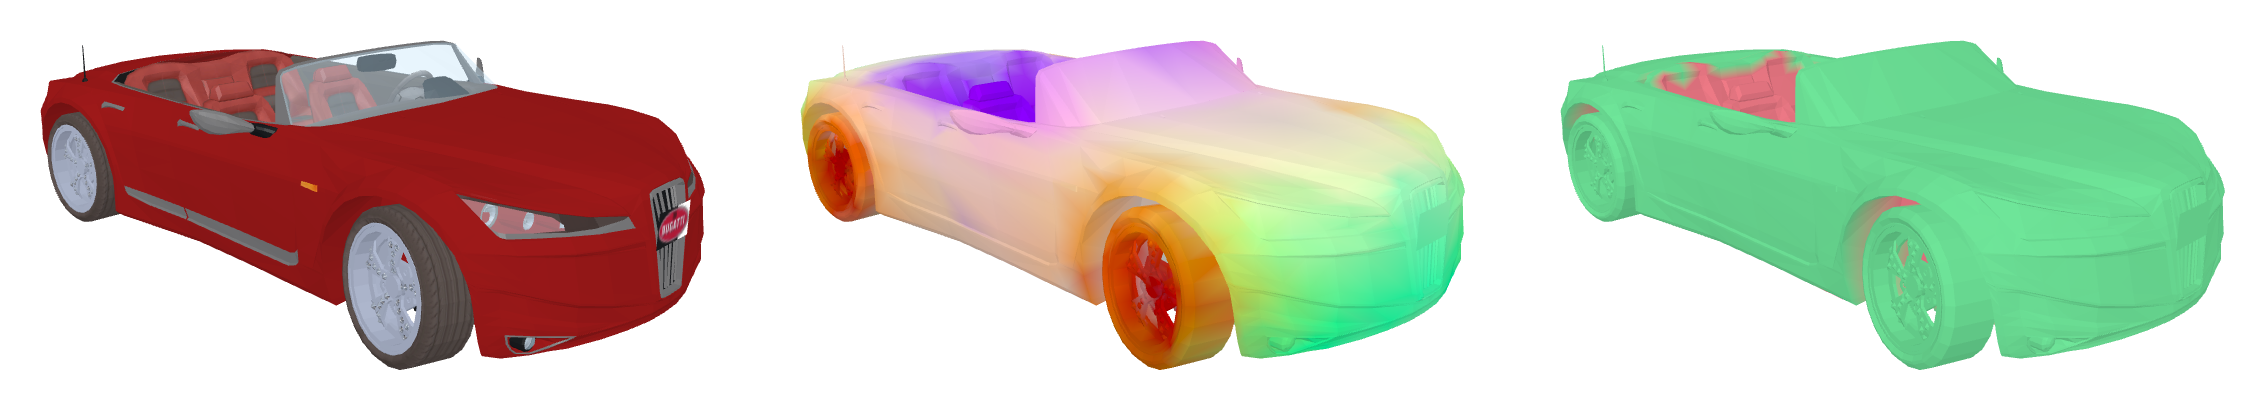
\includegraphics[width=\linewidth]{figures/semantic_analysis/src_triplet_view1.png}\\[-1mm]
    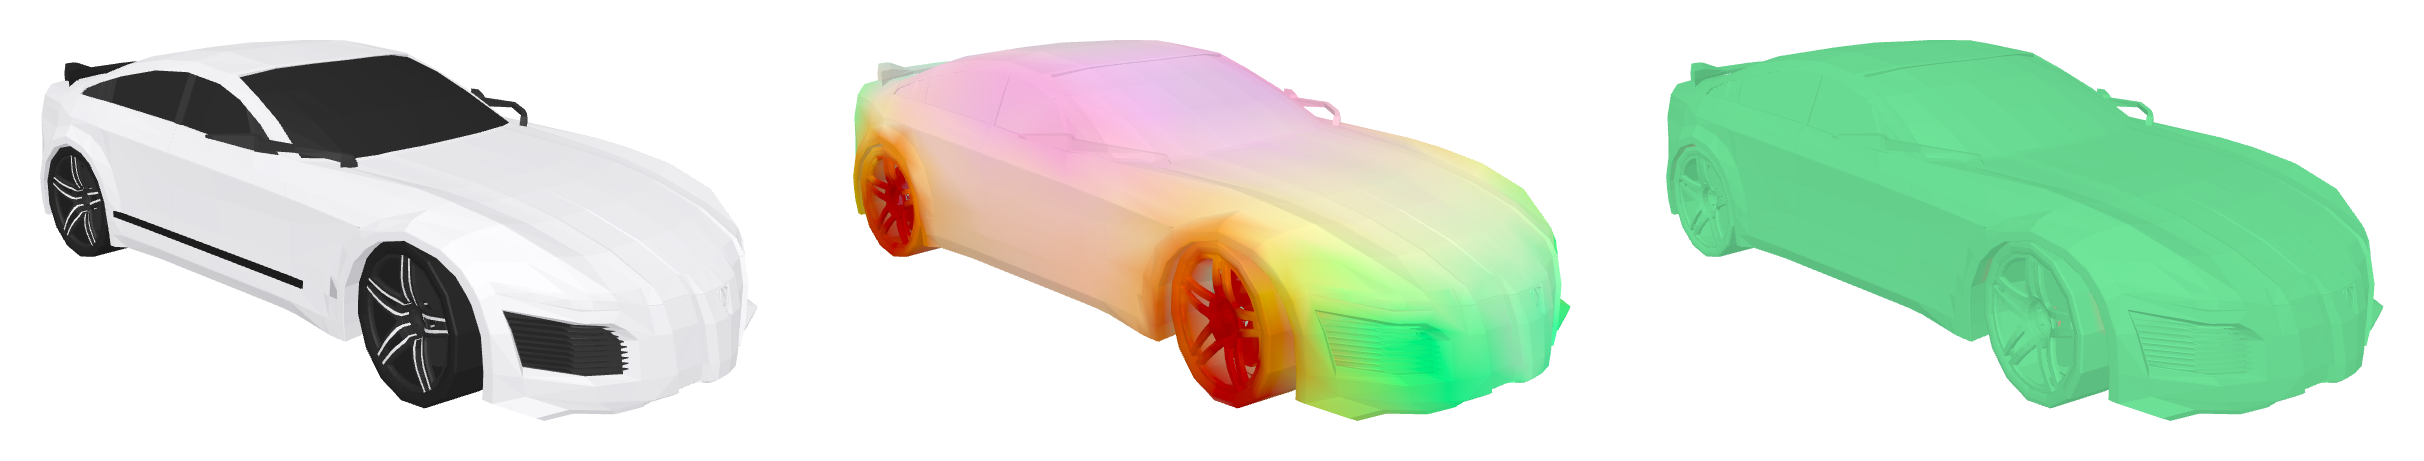
\includegraphics[width=\linewidth]{figures/semantic_analysis/tgt_triplet_view1.png}\\[1mm]
    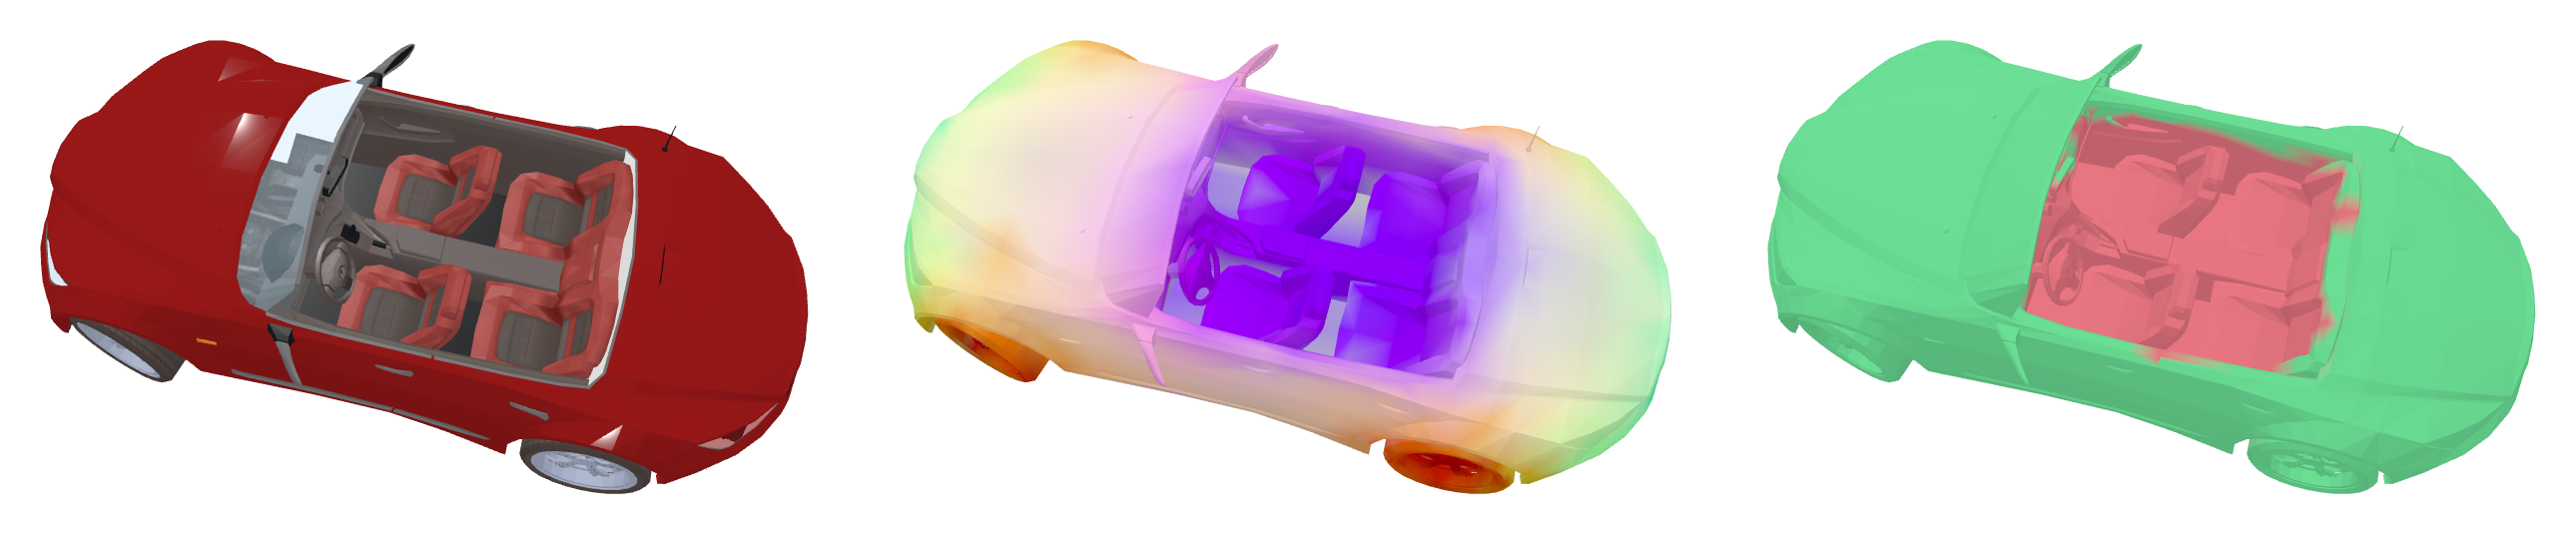
\includegraphics[width=\linewidth]{figures/semantic_analysis/src_triplet_view2.png}\\[-1mm]
    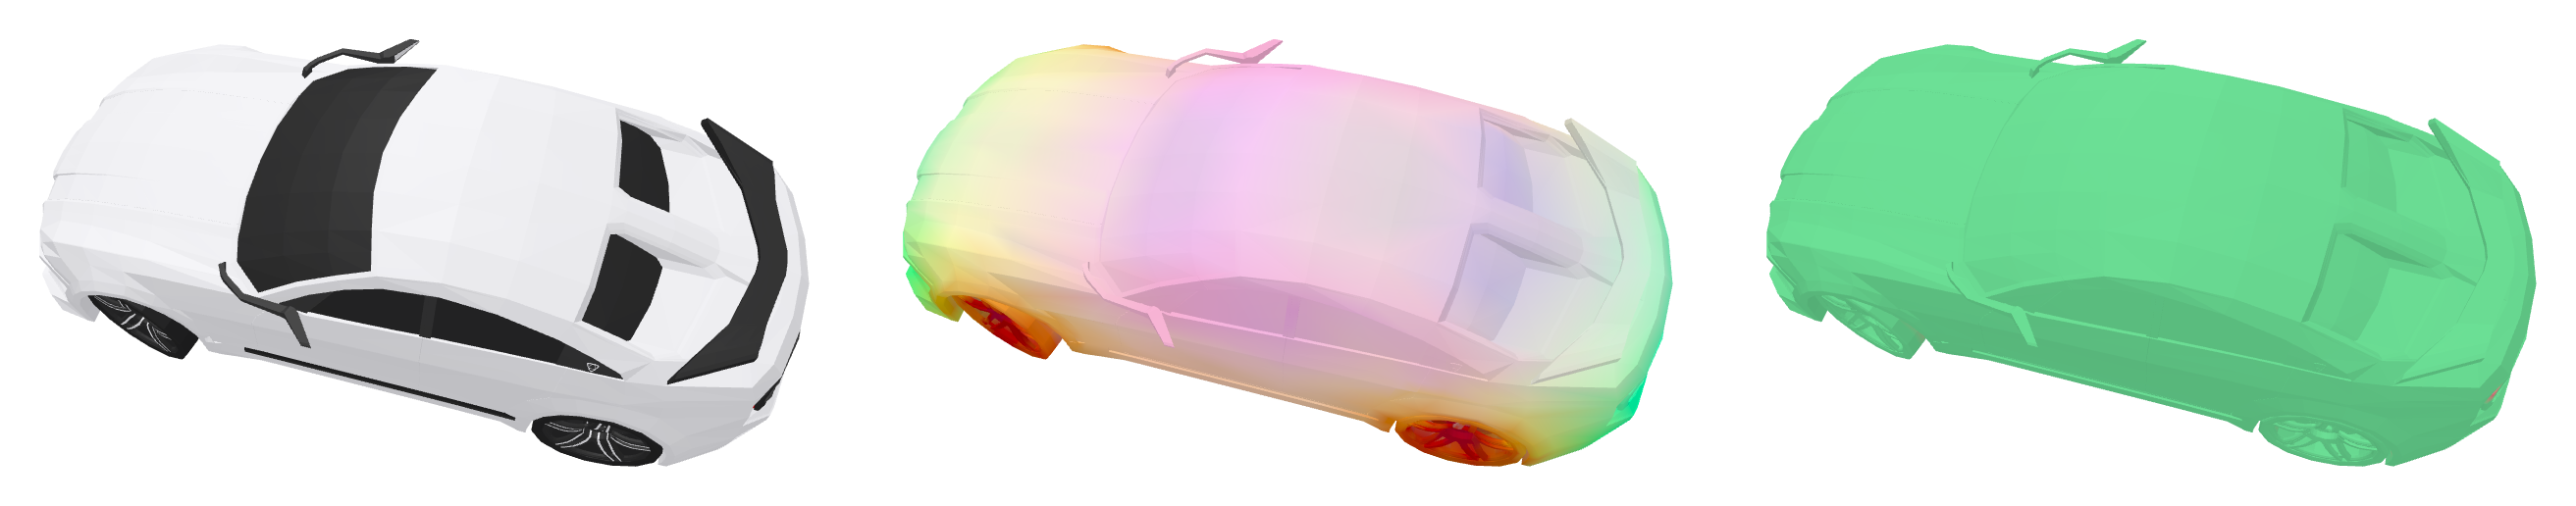
\includegraphics[width=\linewidth]{figures/semantic_analysis/tgt_triplet_view2.png}
\caption{
Qualitative analysis of DINOv2 based semantic coverage. Each row shows the original rendering, a PCA visualization of DINOv2 features computed jointly for the object pair, and the resulting semantic coverage mask. Green points have at least one semantically similar point in the paired object, while red points have none.
}
    
    \label{fig:semantic_coverage_analysis}
\end{figure}


We further visualize sampled correspondences established by our method in \autoref{fig:semantic_correspondence_pruning}. For visualization, we sample farthest points from the final correspondence set after semantic pruning. Each row shows a different view of the same object pair. As can be seen, semantically unmatched regions such as the exposed seats and steering wheel of the roofless car do not obtain correspondences. Similarly, the roof region of the white car is also removed, even though the CPA registration geometrically deforms these regions toward other object parts. These correspondences are filtered by our semantic correspondence pruning stage due to semantic inconsistency.
\clearpage
\begin{figure}[t]
    \centering
    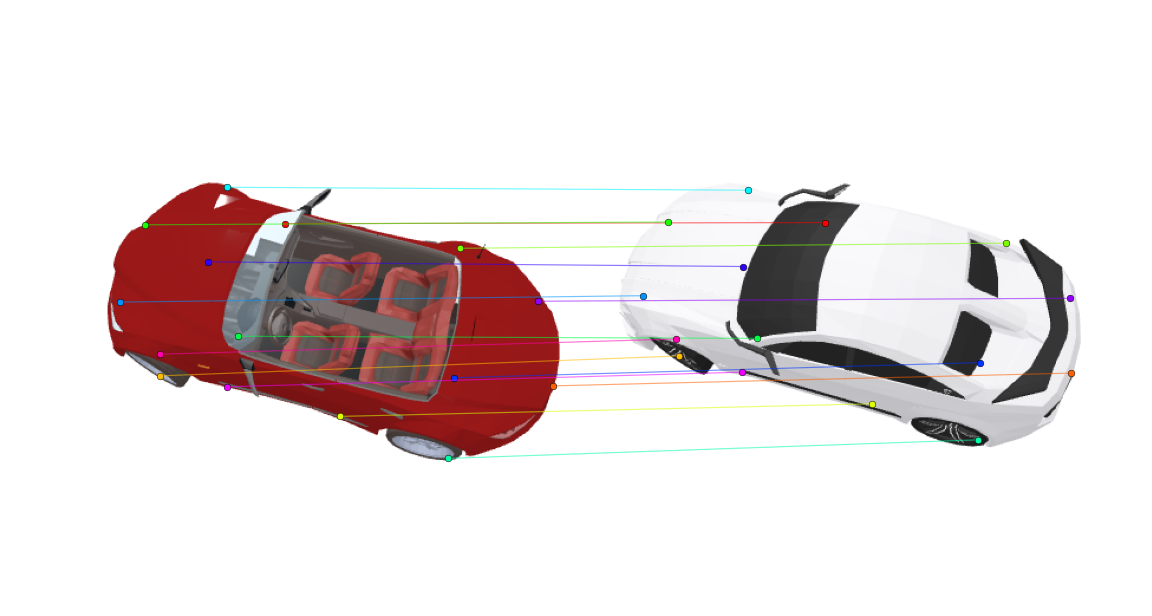
\includegraphics[
        width=0.9\linewidth,
        height=0.26\textheight,
        keepaspectratio,
        trim={20pt 80pt 20pt 80pt},
        clip
    ]{figures/semantic_analysis/sparse15_view10.png}\\[-2mm]
    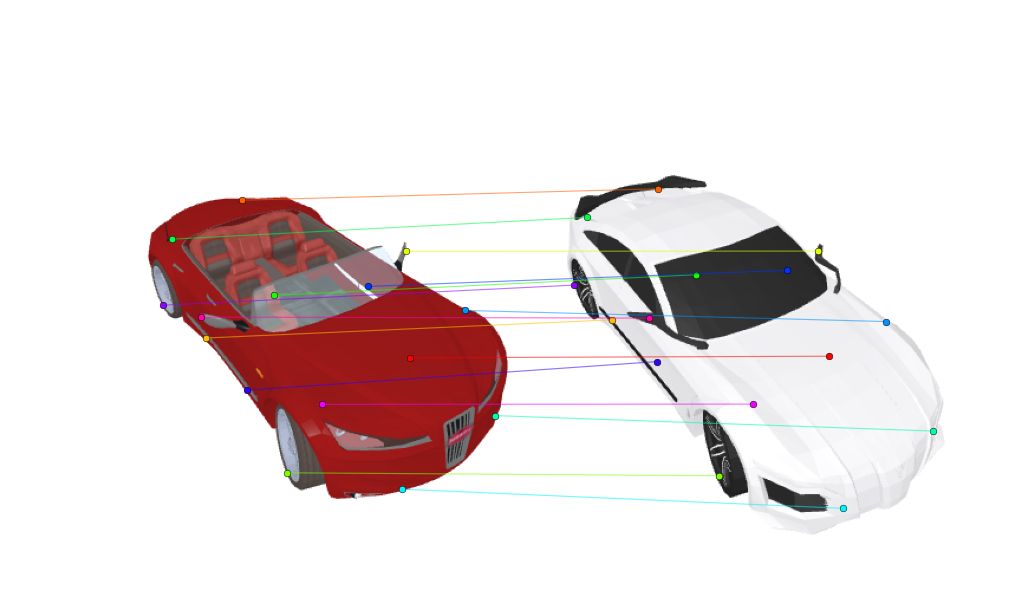
\includegraphics[
        width=0.9\linewidth,
        height=0.26\textheight,
        keepaspectratio,
        trim={20pt 50pt 20pt 80pt},
        clip
    ]{figures/semantic_analysis/sparse15_view34.png}
    \caption{
    Sampled correspondences after semantic pruning. Each row shows a different view of the same object pair.
    }
    \label{fig:semantic_correspondence_pruning}
\end{figure}

\section{Detailed PCK Results by Semantic Label and KeypointNet Category}
\label{Sup:per_label}

We provide a detailed analysis of correspondence quality at the level of individual semantic keypoints. For each category, we evaluate up to 100 objects and all induced source-target pairs, corresponding to up to $\binom{100}{2}$ object pairs per category, across 16 categories and 79,200 pairs overall. We report PCK results per annotated semantic label, following the KeypointNet \cite{you2020} evaluation protocol.

These results are computed using our full pipeline, including correspondence-level semantic filtering with $\tau_{\mathrm{sem}}=0.85$ and pair-level filtering. For each semantic label, we report results as $\text{correct}/\text{total}$, where \emph{total} denotes the number of ground-truth keypoints that remain evaluable after filtering. A keypoint is considered evaluable if at least one predicted correspondence remains within $0.05$ of the object bounding-box diagonal from the ground-truth location. We report raw $\text{correct}/\text{total}$ counts rather than percentages to make the amount of retained evaluable annotations explicit for each semantic label.

KeypointNet annotations are sparse and typically located on salient corners or extreme parts, while our method produces dense correspondences across the object surface. Therefore, these per-label results should be interpreted as a conservative estimate of correspondence quality around the sparse annotated locations.

The full per-label results are reported in 
Tables~\ref{tab:pck_airplane}-\ref{tab:pck_vessel}.


\subimport{./sup_mat/tables}{labels_airplane}

%shira added
\clearpage
\subimport{./sup_mat/tables}{semantic_thresh_values_tables}

% \clearpage
% \subimport{./sup_mat/figures}{keypointnet_fig}
% \subimport{./sup_mat/figures}{failure_cases_keypointnet}

\begin{comment}
        \item[\autoref{Sup:MoreExpRes}.] Additional experiments and results:
            \begin{enumerate}[label=\arabic*)] 
                \item Comparisons on $N=3$ cases (\autoref{fig:triplets})
                \item Camera overlap expressiveness  (\autoref{Fig:5cam}).
                \item Fast Moving Videos from  StabStitch-D dataset ~\cite{Nie:ECCV:2024:stabstitch} (\autoref{fig:fm})
            \end{enumerate}
         \refstepcounter{enumi}   
        \item [\autoref{Sup:ArchN=3}.] An example MVS architecture Plot for an $N>2$ case (\autoref{Fig:method})
        \refstepcounter{enumi}
        \item[\autoref{sec:geovar}.] The Geometric Variance metric
        \refstepcounter{enumi}
        \item[\autoref{sec:arch}.] Additional architecture details: AE and the Alignment Network
\setcounter{figure}{4}
\setcounter{table}{3}      % 4 + 1 → 5
\clearpage

\section{Additional Experiments and Results}\label{Sup:MoreExpRes}
\subimport{./supp_mat/}{experiments_and_results}

\clearpage


\section{An Example for the MVS Architecture for an $N>2$ Case}\label{Sup:ArchN=3}
In the paper, due to page
limit, we show a visualization of 
our MVS architecture
for the case of $N=2$. 
The case of $N>2$ is handled
similarly: in the prepossessing the DINO, PCA and AE steps are still done per cameras,
while the ORT extraction
is still done in a pairwise
fashion. 
Stage 1, based on the geometric loss, utilized 
all the relevant pairs. 
Similarly, this is also the case in Stage 2, where,
for every $t$, 
there are now 3 pairs 
for each time step $t$,
along with three temporal pairs (for $t$ and $t+1$
in each of the $N=3$ cameras).
The architecture,
by design, naturally generalizes
to the case of even 
higher $N$ values. 

\subimport{./supp_mat/}{fig_method} 

\clearpage

\section{The Geometric Variance metric}
\label{sec:geovar}
\subimport{./supp_mat/}{geometric_variance} 
\clearpage

\subimport{./supp_mat/}{arch_details} 


\clearpage
\bibliography{refs}
%\bibliographystyle{abbrvnat}
\bibliographystyle{unsrt}
\end{comment}
% \end{document}

\clearpage

\section*{NeurIPS Paper Checklist}

\begin{enumerate}

\item {\bf Claims}
    \item[] Question: Do the main claims made in the abstract and introduction accurately reflect the paper's contributions and scope?
    \item[] Answer: \answerYes{} % Replace by \answerYes{}, \answerNo{}, or \answerNA{}.
    \item[] Justification: The claims are consistent with the paper’s method, experiments, and reported results.
    \item[] Guidelines:
    \begin{itemize}
        \item The answer \answerNA{} means that the abstract and introduction do not include the claims made in the paper.
        \item The abstract and/or introduction should clearly state the claims made, including the contributions made in the paper and important assumptions and limitations. A \answerNo{} or \answerNA{} answer to this question will not be perceived well by the reviewers. 
        \item The claims made should match theoretical and experimental results, and reflect how much the results can be expected to generalize to other settings. 
        \item It is fine to include aspirational goals as motivation as long as it is clear that these goals are not attained by the paper. 
    \end{itemize}

\item {\bf Limitations}
    \item[] Question: Does the paper discuss the limitations of the work performed by the authors?
    \item[] Answer: \answerYes{} % Replace by \answerYes{}, \answerNo{}, or \answerNA{}.
    \item[] Justification: Yes, the limitations are discussed in Section 4.5. 
    \item[] Guidelines:
    \begin{itemize}
        \item The answer \answerNA{} means that the paper has no limitation while the answer \answerNo{} means that the paper has limitations, but those are not discussed in the paper. 
        \item The authors are encouraged to create a separate ``Limitations'' section in their paper.
        \item The paper should point out any strong assumptions and how robust the results are to violations of these assumptions (e.g., independence assumptions, noiseless settings, model well-specification, asymptotic approximations only holding locally). The authors should reflect on how these assumptions might be violated in practice and what the implications would be.
        \item The authors should reflect on the scope of the claims made, e.g., if the approach was only tested on a few datasets or with a few runs. In general, empirical results often depend on implicit assumptions, which should be articulated.
        \item The authors should reflect on the factors that influence the performance of the approach. For example, a facial recognition algorithm may perform poorly when image resolution is low or images are taken in low lighting. Or a speech-to-text system might not be used reliably to provide closed captions for online lectures because it fails to handle technical jargon.
        \item The authors should discuss the computational efficiency of the proposed algorithms and how they scale with dataset size.
        \item If applicable, the authors should discuss possible limitations of their approach to address problems of privacy and fairness.
        \item While the authors might fear that complete honesty about limitations might be used by reviewers as grounds for rejection, a worse outcome might be that reviewers discover limitations that aren't acknowledged in the paper. The authors should use their best judgment and recognize that individual actions in favor of transparency play an important role in developing norms that preserve the integrity of the community. Reviewers will be specifically instructed to not penalize honesty concerning limitations.
    \end{itemize}

\item {\bf Theory assumptions and proofs}
    \item[] Question: For each theoretical result, does the paper provide the full set of assumptions and a complete (and correct) proof?
   \item[] Answer: \answerNA{}
\item[] Justification: The paper does not include theoretical results or proofs. 
    \item[] Guidelines:
    \begin{itemize}
        \item The answer \answerNA{} means that the paper does not include theoretical results. 
        \item All the theorems, formulas, and proofs in the paper should be numbered and cross-referenced.
        \item All assumptions should be clearly stated or referenced in the statement of any theorems.
        \item The proofs can either appear in the main paper or the supplemental material, but if they appear in the supplemental material, the authors are encouraged to provide a short proof sketch to provide intuition. 
        \item Inversely, any informal proof provided in the core of the paper should be complemented by formal proofs provided in appendix or supplemental material.
        \item Theorems and Lemmas that the proof relies upon should be properly referenced. 
    \end{itemize}

    \item {\bf Experimental result reproducibility}
    \item[] Question: Does the paper fully disclose all the information needed to reproduce the main experimental results of the paper to the extent that it affects the main claims and/or conclusions of the paper (regardless of whether the code and data are provided or not)?
\item[] Answer: \answerYes{}
\item[] Justification: The paper provides the main implementation, training, and evaluation details needed to reproduce the reported experimental results.
    \item[] Guidelines:
    \begin{itemize}
        \item The answer \answerNA{} means that the paper does not include experiments.
        \item If the paper includes experiments, a \answerNo{} answer to this question will not be perceived well by the reviewers: Making the paper reproducible is important, regardless of whether the code and data are provided or not.
        \item If the contribution is a dataset and\slash or model, the authors should describe the steps taken to make their results reproducible or verifiable. 
        \item Depending on the contribution, reproducibility can be accomplished in various ways. For example, if the contribution is a novel architecture, describing the architecture fully might suffice, or if the contribution is a specific model and empirical evaluation, it may be necessary to either make it possible for others to replicate the model with the same dataset, or provide access to the model. In general. releasing code and data is often one good way to accomplish this, but reproducibility can also be provided via detailed instructions for how to replicate the results, access to a hosted model (e.g., in the case of a large language model), releasing of a model checkpoint, or other means that are appropriate to the research performed.
        \item While NeurIPS does not require releasing code, the conference does require all submissions to provide some reasonable avenue for reproducibility, which may depend on the nature of the contribution. For example
        \begin{enumerate}
            \item If the contribution is primarily a new algorithm, the paper should make it clear how to reproduce that algorithm.
            \item If the contribution is primarily a new model architecture, the paper should describe the architecture clearly and fully.
            \item If the contribution is a new model (e.g., a large language model), then there should either be a way to access this model for reproducing the results or a way to reproduce the model (e.g., with an open-source dataset or instructions for how to construct the dataset).
            \item We recognize that reproducibility may be tricky in some cases, in which case authors are welcome to describe the particular way they provide for reproducibility. In the case of closed-source models, it may be that access to the model is limited in some way (e.g., to registered users), but it should be possible for other researchers to have some path to reproducing or verifying the results.
        \end{enumerate}
    \end{itemize}


\item {\bf Open access to data and code}
    \item[] Question: Does the paper provide open access to the data and code, with sufficient instructions to faithfully reproduce the main experimental results, as described in supplemental material?
\item[] Answer: \answerYes{}
\item[] Justification: The code, data, and reproduction instructions will be released upon acceptance.
    \item[] Guidelines:
    \begin{itemize}
        \item The answer \answerNA{} means that paper does not include experiments requiring code.
        \item Please see the NeurIPS code and data submission guidelines (\url{https://neurips.cc/public/guides/CodeSubmissionPolicy}) for more details.
        \item While we encourage the release of code and data, we understand that this might not be possible, so \answerNo{} is an acceptable answer. Papers cannot be rejected simply for not including code, unless this is central to the contribution (e.g., for a new open-source benchmark).
        \item The instructions should contain the exact command and environment needed to run to reproduce the results. See the NeurIPS code and data submission guidelines (\url{https://neurips.cc/public/guides/CodeSubmissionPolicy}) for more details.
        \item The authors should provide instructions on data access and preparation, including how to access the raw data, preprocessed data, intermediate data, and generated data, etc.
        \item The authors should provide scripts to reproduce all experimental results for the new proposed method and baselines. If only a subset of experiments are reproducible, they should state which ones are omitted from the script and why.
        \item At submission time, to preserve anonymity, the authors should release anonymized versions (if applicable).
        \item Providing as much information as possible in supplemental material (appended to the paper) is recommended, but including URLs to data and code is permitted.
    \end{itemize}


\item {\bf Experimental setting/details}
    \item[] Question: Does the paper specify all the training and test details (e.g., data splits, hyperparameters, how they were chosen, type of optimizer) necessary to understand the results?
\item[] Answer: \answerYes{}
\item[] Justification: The paper specifies the main training, evaluation, and implementation details necessary to understand the reported results.
    \item[] Guidelines:
    \begin{itemize}
        \item The answer \answerNA{} means that the paper does not include experiments.
        \item The experimental setting should be presented in the core of the paper to a level of detail that is necessary to appreciate the results and make sense of them.
        \item The full details can be provided either with the code, in appendix, or as supplemental material.
    \end{itemize}

\item {\bf Experiment statistical significance}
    \item[] Question: Does the paper report error bars suitably and correctly defined or other appropriate information about the statistical significance of the experiments?
\item[] Answer: \answerNo{}
\item[] Justification: The paper does not report error bars or statistical significance analyses.
    \item[] Guidelines:
    \begin{itemize}
        \item The answer \answerNA{} means that the paper does not include experiments.
        \item The authors should answer \answerYes{} if the results are accompanied by error bars, confidence intervals, or statistical significance tests, at least for the experiments that support the main claims of the paper.
        \item The factors of variability that the error bars are capturing should be clearly stated (for example, train/test split, initialization, random drawing of some parameter, or overall run with given experimental conditions).
        \item The method for calculating the error bars should be explained (closed form formula, call to a library function, bootstrap, etc.)
        \item The assumptions made should be given (e.g., Normally distributed errors).
        \item It should be clear whether the error bar is the standard deviation or the standard error of the mean.
        \item It is OK to report 1-sigma error bars, but one should state it. The authors should preferably report a 2-sigma error bar than state that they have a 96\% CI, if the hypothesis of Normality of errors is not verified.
        \item For asymmetric distributions, the authors should be careful not to show in tables or figures symmetric error bars that would yield results that are out of range (e.g., negative error rates).
        \item If error bars are reported in tables or plots, the authors should explain in the text how they were calculated and reference the corresponding figures or tables in the text.
    \end{itemize}

\item {\bf Experiments compute resources}
    \item[] Question: For each experiment, does the paper provide sufficient information on the computer resources (type of compute workers, memory, time of execution) needed to reproduce the experiments?
\item[] Answer: \answerYes{}
\item[] Justification: The paper reports the compute resources required to reproduce the main experiments.
    \item[] Guidelines:
    \begin{itemize}
        \item The answer \answerNA{} means that the paper does not include experiments.
        \item The paper should indicate the type of compute workers CPU or GPU, internal cluster, or cloud provider, including relevant memory and storage.
        \item The paper should provide the amount of compute required for each of the individual experimental runs as well as estimate the total compute. 
        \item The paper should disclose whether the full research project required more compute than the experiments reported in the paper (e.g., preliminary or failed experiments that didn't make it into the paper). 
    \end{itemize}
    
\item {\bf Code of ethics}
    \item[] Question: Does the research conducted in the paper conform, in every respect, with the NeurIPS Code of Ethics \url{https://neurips.cc/public/EthicsGuidelines}?
\item[] Answer: \answerYes{}
\item[] Justification: The research complies with the NeurIPS Code of Ethics.
    \item[] Guidelines:
    \begin{itemize}
        \item The answer \answerNA{} means that the authors have not reviewed the NeurIPS Code of Ethics.
        \item If the authors answer \answerNo, they should explain the special circumstances that require a deviation from the Code of Ethics.
        \item The authors should make sure to preserve anonymity (e.g., if there is a special consideration due to laws or regulations in their jurisdiction).
    \end{itemize}


\item {\bf Broader impacts}
    \item[] Question: Does the paper discuss both potential positive societal impacts and negative societal impacts of the work performed?
\item[] Answer: \answerNo{}
\item[] Justification: The paper focuses on a technical data generation pipeline and does not identify societal impacts specific to this task beyond those generally associated with standard computer vision methods.
    \item[] Guidelines:
    \begin{itemize}
        \item The answer \answerNA{} means that there is no societal impact of the work performed.
        \item If the authors answer \answerNA{} or \answerNo, they should explain why their work has no societal impact or why the paper does not address societal impact.
        \item Examples of negative societal impacts include potential malicious or unintended uses (e.g., disinformation, generating fake profiles, surveillance), fairness considerations (e.g., deployment of technologies that could make decisions that unfairly impact specific groups), privacy considerations, and security considerations.
        \item The conference expects that many papers will be foundational research and not tied to particular applications, let alone deployments. However, if there is a direct path to any negative applications, the authors should point it out. For example, it is legitimate to point out that an improvement in the quality of generative models could be used to generate Deepfakes for disinformation. On the other hand, it is not needed to point out that a generic algorithm for optimizing neural networks could enable people to train models that generate Deepfakes faster.
        \item The authors should consider possible harms that could arise when the technology is being used as intended and functioning correctly, harms that could arise when the technology is being used as intended but gives incorrect results, and harms following from (intentional or unintentional) misuse of the technology.
        \item If there are negative societal impacts, the authors could also discuss possible mitigation strategies (e.g., gated release of models, providing defenses in addition to attacks, mechanisms for monitoring misuse, mechanisms to monitor how a system learns from feedback over time, improving the efficiency and accessibility of ML).
    \end{itemize}
    
\item {\bf Safeguards}
    \item[] Question: Does the paper describe safeguards that have been put in place for responsible release of data or models that have a high risk for misuse (e.g., pre-trained language models, image generators, or scraped datasets)?
\item[] Answer: \answerNA{}
\item[] Justification: The work does not release data or models with a high risk for misuse, such as pretrained language models, image generators, or scraped sensitive datasets.
    \item[] Guidelines:
    \begin{itemize}
        \item The answer \answerNA{} means that the paper poses no such risks.
        \item Released models that have a high risk for misuse or dual-use should be released with necessary safeguards to allow for controlled use of the model, for example by requiring that users adhere to usage guidelines or restrictions to access the model or implementing safety filters. 
        \item Datasets that have been scraped from the Internet could pose safety risks. The authors should describe how they avoided releasing unsafe images.
        \item We recognize that providing effective safeguards is challenging, and many papers do not require this, but we encourage authors to take this into account and make a best faith effort.
    \end{itemize}

\item {\bf Licenses for existing assets}
    \item[] Question: Are the creators or original owners of assets (e.g., code, data, models), used in the paper, properly credited and are the license and terms of use explicitly mentioned and properly respected?
\item[] Answer: \answerYes{}
\item[] Justification: The original datasets, codebases, and assets used in the paper are properly credited. The corresponding licenses and terms of use will be included with the released code and data.
    \item[] Guidelines:
    \begin{itemize}
        \item The answer \answerNA{} means that the paper does not use existing assets.
        \item The authors should cite the original paper that produced the code package or dataset.
        \item The authors should state which version of the asset is used and, if possible, include a URL.
        \item The name of the license (e.g., CC-BY 4.0) should be included for each asset.
        \item For scraped data from a particular source (e.g., website), the copyright and terms of service of that source should be provided.
        \item If assets are released, the license, copyright information, and terms of use in the package should be provided. For popular datasets, \url{paperswithcode.com/datasets} has curated licenses for some datasets. Their licensing guide can help determine the license of a dataset.
        \item For existing datasets that are re-packaged, both the original license and the license of the derived asset (if it has changed) should be provided.
        \item If this information is not available online, the authors are encouraged to reach out to the asset's creators.
    \end{itemize}

\item {\bf New assets}
    \item[] Question: Are new assets introduced in the paper well documented and is the documentation provided alongside the assets?
\item[] Answer: \answerYes{}
\item[] Justification: The new assets introduced in the paper are documented and will be released together with the corresponding code and data.
    \item[] Guidelines:
    \begin{itemize}
        \item The answer \answerNA{} means that the paper does not release new assets.
        \item Researchers should communicate the details of the dataset\slash code\slash model as part of their submissions via structured templates. This includes details about training, license, limitations, etc. 
        \item The paper should discuss whether and how consent was obtained from people whose asset is used.
        \item At submission time, remember to anonymize your assets (if applicable). You can either create an anonymized URL or include an anonymized zip file.
    \end{itemize}

\item {\bf Crowdsourcing and research with human subjects}
    \item[] Question: For crowdsourcing experiments and research with human subjects, does the paper include the full text of instructions given to participants and screenshots, if applicable, as well as details about compensation (if any)? 
\item[] Answer: \answerNA{}
\item[] Justification: The paper does not involve crowdsourcing experiments or research with human subjects.
    \item[] Guidelines:
    \begin{itemize}
        \item The answer \answerNA{} means that the paper does not involve crowdsourcing nor research with human subjects.
        \item Including this information in the supplemental material is fine, but if the main contribution of the paper involves human subjects, then as much detail as possible should be included in the main paper. 
        \item According to the NeurIPS Code of Ethics, workers involved in data collection, curation, or other labor should be paid at least the minimum wage in the country of the data collector. 
    \end{itemize}

\item {\bf Institutional review board (IRB) approvals or equivalent for research with human subjects}
    \item[] Question: Does the paper describe potential risks incurred by study participants, whether such risks were disclosed to the subjects, and whether Institutional Review Board (IRB) approvals (or an equivalent approval/review based on the requirements of your country or institution) were obtained?
\item[] Answer: \answerNA{}
\item[] Justification: The paper does not involve research with human subjects requiring IRB approval.
    \item[] Guidelines:
    \begin{itemize}
        \item The answer \answerNA{} means that the paper does not involve crowdsourcing nor research with human subjects.
        \item Depending on the country in which research is conducted, IRB approval (or equivalent) may be required for any human subjects research. If you obtained IRB approval, you should clearly state this in the paper. 
        \item We recognize that the procedures for this may vary significantly between institutions and locations, and we expect authors to adhere to the NeurIPS Code of Ethics and the guidelines for their institution. 
        \item For initial submissions, do not include any information that would break anonymity (if applicable), such as the institution conducting the review.
    \end{itemize}

\item {\bf Declaration of LLM usage}
    \item[] Question: Does the paper describe the usage of LLMs if it is an important, original, or non-standard component of the core methods in this research? Note that if the LLM is used only for writing, editing, or formatting purposes and does \emph{not} impact the core methodology, scientific rigor, or originality of the research, declaration is not required.
    %this research? 
\item[] Answer: \answerNA{}
\item[] Justification: LLMs were not used as part of the core research methodology.
    \item[] Guidelines:
    \begin{itemize}
        \item The answer \answerNA{} means that the core method development in this research does not involve LLMs as any important, original, or non-standard components.
        \item Please refer to our LLM policy in the NeurIPS handbook for what should or should not be described.
    \end{itemize}

\end{enumerate}
% \appendix

% \section{Additional implementation details}

% In the supplementary material, we provide additional implementation details, qualitative examples of generated correspondences, statistics for each category, and ablations on correspondence filtering and rendering choices.

\end{document}